\documentclass[twoside]{book}

% Packages required by doxygen
\usepackage{fixltx2e}
\usepackage{calc}
\usepackage{doxygen}
\usepackage[export]{adjustbox} % also loads graphicx
\usepackage{graphicx}
\usepackage[utf8]{inputenc}
\usepackage{makeidx}
\usepackage{multicol}
\usepackage{multirow}
\PassOptionsToPackage{warn}{textcomp}
\usepackage{textcomp}
\usepackage[nointegrals]{wasysym}
\usepackage[table]{xcolor}

% NLS support packages
Portuguese
% Font selection
\usepackage[T1]{fontenc}
\usepackage[scaled=.90]{helvet}
\usepackage{courier}
\usepackage{amssymb}
\usepackage{sectsty}
\renewcommand{\familydefault}{\sfdefault}
\allsectionsfont{%
  \fontseries{bc}\selectfont%
  \color{darkgray}%
}
\renewcommand{\DoxyLabelFont}{%
  \fontseries{bc}\selectfont%
  \color{darkgray}%
}
\newcommand{\+}{\discretionary{\mbox{\scriptsize$\hookleftarrow$}}{}{}}

% Page & text layout
\usepackage{geometry}
\geometry{%
  a4paper,%
  top=2.5cm,%
  bottom=2.5cm,%
  left=2.5cm,%
  right=2.5cm%
}
\tolerance=750
\hfuzz=15pt
\hbadness=750
\setlength{\emergencystretch}{15pt}
\setlength{\parindent}{0cm}
\setlength{\parskip}{3ex plus 2ex minus 2ex}
\makeatletter
\renewcommand{\paragraph}{%
  \@startsection{paragraph}{4}{0ex}{-1.0ex}{1.0ex}{%
    \normalfont\normalsize\bfseries\SS@parafont%
  }%
}
\renewcommand{\subparagraph}{%
  \@startsection{subparagraph}{5}{0ex}{-1.0ex}{1.0ex}{%
    \normalfont\normalsize\bfseries\SS@subparafont%
  }%
}
\makeatother

% Headers & footers
\usepackage{fancyhdr}
\pagestyle{fancyplain}
\fancyhead[LE]{\fancyplain{}{\bfseries\thepage}}
\fancyhead[CE]{\fancyplain{}{}}
\fancyhead[RE]{\fancyplain{}{\bfseries\leftmark}}
\fancyhead[LO]{\fancyplain{}{\bfseries\rightmark}}
\fancyhead[CO]{\fancyplain{}{}}
\fancyhead[RO]{\fancyplain{}{\bfseries\thepage}}
\fancyfoot[LE]{\fancyplain{}{}}
\fancyfoot[CE]{\fancyplain{}{}}
\fancyfoot[RE]{\fancyplain{}{\bfseries\scriptsize Gerado por Doxygen }}
\fancyfoot[LO]{\fancyplain{}{\bfseries\scriptsize Gerado por Doxygen }}
\fancyfoot[CO]{\fancyplain{}{}}
\fancyfoot[RO]{\fancyplain{}{}}
\renewcommand{\footrulewidth}{0.4pt}
\renewcommand{\chaptermark}[1]{%
  \markboth{#1}{}%
}
\renewcommand{\sectionmark}[1]{%
  \markright{\thesection\ #1}%
}

% Indices & bibliography
\usepackage{natbib}
\usepackage[titles]{tocloft}
\setcounter{tocdepth}{3}
\setcounter{secnumdepth}{5}
\makeindex

% Hyperlinks (required, but should be loaded last)
\usepackage{ifpdf}
\ifpdf
  \usepackage[pdftex,pagebackref=true]{hyperref}
\else
  \usepackage[ps2pdf,pagebackref=true]{hyperref}
\fi
\hypersetup{%
  colorlinks=true,%
  linkcolor=blue,%
  citecolor=blue,%
  unicode%
}

% Custom commands
\newcommand{\clearemptydoublepage}{%
  \newpage{\pagestyle{empty}\cleardoublepage}%
}

\usepackage{caption}
\captionsetup{labelsep=space,justification=centering,font={bf},singlelinecheck=off,skip=4pt,position=top}

%===== C O N T E N T S =====

\begin{document}

% Titlepage & ToC
\hypersetup{pageanchor=false,
             bookmarksnumbered=true,
             pdfencoding=unicode
            }
\pagenumbering{alph}
\begin{titlepage}
\vspace*{7cm}
\begin{center}%
{\Large Java Virtual Machine }\\
\vspace*{1cm}
{\large Gerado por Doxygen 1.8.13}\\
\end{center}
\end{titlepage}
\clearemptydoublepage
\pagenumbering{roman}
\tableofcontents
\clearemptydoublepage
\pagenumbering{arabic}
\hypersetup{pageanchor=true}

%--- Begin generated contents ---
\chapter{Índice das estruturas de dados}
\section{Estruturas de dados}
Lista das estruturas de dados com uma breve descrição\+:\begin{DoxyCompactList}
\item\contentsline{section}{\hyperlink{structattribute__info}{attribute\+\_\+info} \\*Estrutura de dados para salvar a posição do atributo na constantpool e seu tamanho }{\pageref{structattribute__info}}{}
\item\contentsline{section}{\hyperlink{classClasseEstatica}{Classe\+Estatica} \\*Fields Estáticos compartilhados por todas as instâncias }{\pageref{classClasseEstatica}}{}
\item\contentsline{section}{\hyperlink{classClasseInstancia}{Classe\+Instancia} \\*Class instantiation }{\pageref{classClasseInstancia}}{}
\item\contentsline{section}{\hyperlink{unionClassLoaderType}{Class\+Loader\+Type} \\*Estrutura de dados para armazenamento Union responsável por armazenar todos os tamanhos de variáveis utilzadas na J\+VM }{\pageref{unionClassLoaderType}}{}
\item\contentsline{section}{\hyperlink{structcode__attribute}{code\+\_\+attribute} \\*Estrutura de dados para salvar atributos do tipo code }{\pageref{structcode__attribute}}{}
\item\contentsline{section}{\hyperlink{structconstantvalue__attribute}{constantvalue\+\_\+attribute} \\*Struct para carregar o index dos atributos da \char`\"{}constantpool\char`\"{} }{\pageref{structconstantvalue__attribute}}{}
\item\contentsline{section}{\hyperlink{structcp__info}{cp\+\_\+info} \\*Possui um elemento pool de constante }{\pageref{structcp__info}}{}
\item\contentsline{section}{\hyperlink{unionelement__u}{element\+\_\+u} \\*Generalização de funções de retorno/input Union responsável pela generalização de funções de retorno e uma função de input }{\pageref{unionelement__u}}{}
\item\contentsline{section}{\hyperlink{structexception__attribute}{exception\+\_\+attribute} }{\pageref{structexception__attribute}}{}
\item\contentsline{section}{\hyperlink{structfield__info}{field\+\_\+info} \\*Struct de armazenamento }{\pageref{structfield__info}}{}
\item\contentsline{section}{\hyperlink{structframe__s}{frame\+\_\+s} \\*Estrutura de armazenamento }{\pageref{structframe__s}}{}
\item\contentsline{section}{\hyperlink{classFrameStack}{Frame\+Stack} \\*Classe de pilha de frames }{\pageref{classFrameStack}}{}
\item\contentsline{section}{\hyperlink{classHeap}{Heap} \\*Classe do heap }{\pageref{classHeap}}{}
\item\contentsline{section}{\hyperlink{classLeitor}{Leitor} }{\pageref{classLeitor}}{}
\item\contentsline{section}{\hyperlink{classLocalVariables}{Local\+Variables} \\*Local variables Class }{\pageref{classLocalVariables}}{}
\item\contentsline{section}{\hyperlink{structmethod__info}{method\+\_\+info} }{\pageref{structmethod__info}}{}
\item\contentsline{section}{\hyperlink{classMethodArea}{Method\+Area} \\*Classe responsável por todas as operações que gerenciam os métodos }{\pageref{classMethodArea}}{}
\item\contentsline{section}{\hyperlink{structn__array}{n\+\_\+array} }{\pageref{structn__array}}{}
\item\contentsline{section}{\hyperlink{classOperacoes}{Operacoes} }{\pageref{classOperacoes}}{}
\item\contentsline{section}{\hyperlink{classPilhaOperandos}{Pilha\+Operandos} \\*Classe da pilha de operandos }{\pageref{classPilhaOperandos}}{}
\item\contentsline{section}{\hyperlink{structt__exception__table}{t\+\_\+exception\+\_\+table} \\*Struct para salvar exceções identificadas. Será utilizada como componente da struct \char`\"{}code\+\_\+attribute\char`\"{} }{\pageref{structt__exception__table}}{}
\item\contentsline{section}{\hyperlink{uniont__info}{t\+\_\+info} \\*Estrutura de dados que agrega informações sobre cada atributo lido }{\pageref{uniont__info}}{}
\item\contentsline{section}{\hyperlink{structtypedElement__s}{typed\+Element\+\_\+s} \\*Agregador de tipos e informações. Struct responsável por juntar tipos e informações de elementos }{\pageref{structtypedElement__s}}{}
\end{DoxyCompactList}

\chapter{Índice dos ficheiros}
\section{Lista de ficheiros}
Lista de todos os ficheiros documentados com uma breve descrição\+:\begin{DoxyCompactList}
\item\contentsline{section}{include/\hyperlink{attributes_8h}{attributes.\+h} \\*Atributos a serem usados na execuçao da J\+VM }{\pageref{attributes_8h}}{}
\item\contentsline{section}{include/\hyperlink{baseTypes_8h}{base\+Types.\+h} \\*Tipos Base Tipos básicos utilizados para implementarmos a J\+VM }{\pageref{baseTypes_8h}}{}
\item\contentsline{section}{include/\hyperlink{classe_8h}{classe.\+h} \\*Definição da \hyperlink{classClasseEstatica}{Classe\+Estatica} e da \hyperlink{classClasseInstancia}{Classe\+Instancia} }{\pageref{classe_8h}}{}
\item\contentsline{section}{include/\hyperlink{classeLeitor_8h}{classe\+Leitor.\+h} }{\pageref{classeLeitor_8h}}{}
\item\contentsline{section}{include/\hyperlink{classFlags_8h}{class\+Flags.\+h} \\*Class Flags }{\pageref{classFlags_8h}}{}
\item\contentsline{section}{include/\hyperlink{constantPool_8h}{constant\+Pool.\+h} \\*Módulo Constant pool }{\pageref{constantPool_8h}}{}
\item\contentsline{section}{include/\hyperlink{fields_8h}{fields.\+h} \\*Classe field }{\pageref{fields_8h}}{}
\item\contentsline{section}{include/\hyperlink{frame_8h}{frame.\+h} \\*Contém tudo necessário para a execução de um método }{\pageref{frame_8h}}{}
\item\contentsline{section}{include/\hyperlink{heap_8h}{heap.\+h} \\*Definição do \hyperlink{classHeap}{Heap} }{\pageref{heap_8h}}{}
\item\contentsline{section}{include/\hyperlink{interfaces_8h}{interfaces.\+h} \\*Interfaces }{\pageref{interfaces_8h}}{}
\item\contentsline{section}{include/\hyperlink{localVariables_8h}{local\+Variables.\+h} \\*Local Variables }{\pageref{localVariables_8h}}{}
\item\contentsline{section}{include/{\bfseries method\+Area.\+h} }{\pageref{methodArea_8h}}{}
\item\contentsline{section}{include/{\bfseries methods.\+h} }{\pageref{methods_8h}}{}
\item\contentsline{section}{include/{\bfseries operacoes.\+h} }{\pageref{operacoes_8h}}{}
\item\contentsline{section}{include/\hyperlink{pilhaOperandos_8h}{pilha\+Operandos.\+h} \\*Pilha de operandos }{\pageref{pilhaOperandos_8h}}{}
\item\contentsline{section}{src/\hyperlink{attributes_8cpp}{attributes.\+cpp} \\*Attributes.\+cpp }{\pageref{attributes_8cpp}}{}
\item\contentsline{section}{src/\hyperlink{baseTypes_8cpp}{base\+Types.\+cpp} \\*Basetypes.\+cpp }{\pageref{baseTypes_8cpp}}{}
\item\contentsline{section}{src/\hyperlink{classe_8cpp}{classe.\+cpp} \\*Classe.\+cpp }{\pageref{classe_8cpp}}{}
\item\contentsline{section}{src/\hyperlink{classeLeitor_8cpp}{classe\+Leitor.\+cpp} \\*Classe\+Leitor.\+cpp }{\pageref{classeLeitor_8cpp}}{}
\item\contentsline{section}{src/\hyperlink{classFlags_8cpp}{class\+Flags.\+cpp} \\*Class\+Flags.\+cpp }{\pageref{classFlags_8cpp}}{}
\item\contentsline{section}{src/\hyperlink{constantPool_8cpp}{constant\+Pool.\+cpp} \\*Constant\+Pool.\+cpp }{\pageref{constantPool_8cpp}}{}
\item\contentsline{section}{src/\hyperlink{fields_8cpp}{fields.\+cpp} \\*Fields.\+cpp }{\pageref{fields_8cpp}}{}
\item\contentsline{section}{src/\hyperlink{frame_8cpp}{frame.\+cpp} }{\pageref{frame_8cpp}}{}
\item\contentsline{section}{src/\hyperlink{heap_8cpp}{heap.\+cpp} }{\pageref{heap_8cpp}}{}
\item\contentsline{section}{src/\hyperlink{interfaces_8cpp}{interfaces.\+cpp} \\*Interfaces }{\pageref{interfaces_8cpp}}{}
\item\contentsline{section}{src/\hyperlink{localVariables_8cpp}{local\+Variables.\+cpp} }{\pageref{localVariables_8cpp}}{}
\item\contentsline{section}{src/\hyperlink{main_8cpp}{main.\+cpp} }{\pageref{main_8cpp}}{}
\item\contentsline{section}{src/\hyperlink{methods_8cpp}{methods.\+cpp} }{\pageref{methods_8cpp}}{}
\item\contentsline{section}{src/\hyperlink{operacoes_8cpp}{operacoes.\+cpp} }{\pageref{operacoes_8cpp}}{}
\item\contentsline{section}{src/\hyperlink{pilhaOperandos_8cpp}{pilha\+Operandos.\+cpp} \\*Pilha de operandos }{\pageref{pilhaOperandos_8cpp}}{}
\end{DoxyCompactList}

\chapter{Documentação da classe}
\hypertarget{structattribute__info}{}\section{Referência à estrutura attribute\+\_\+info}
\label{structattribute__info}\index{attribute\+\_\+info@{attribute\+\_\+info}}


Estrutura de dados para salvar a posição do atributo na constantpool e seu tamanho.  




{\ttfamily \#include $<$attributes.\+h$>$}



Diagrama de colaboração para attribute\+\_\+info\+:
\nopagebreak
\begin{figure}[H]
\begin{center}
\leavevmode
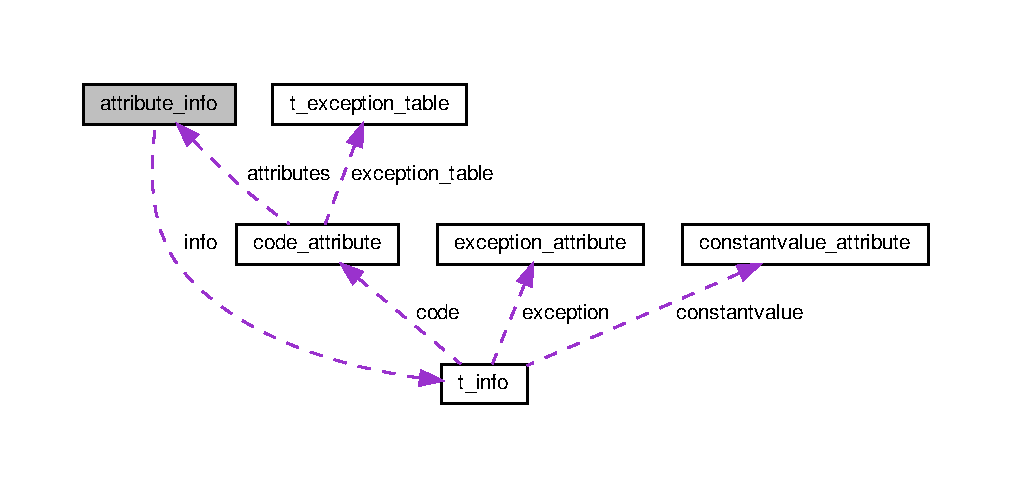
\includegraphics[width=350pt]{structattribute__info__coll__graph}
\end{center}
\end{figure}
\subsection*{Campos de Dados}
\begin{DoxyCompactItemize}
\item 
\mbox{\Hypertarget{structattribute__info_ac90a7f38d57c03dd9b213a4191fdfe0f}\label{structattribute__info_ac90a7f38d57c03dd9b213a4191fdfe0f}} 
unsigned short {\bfseries name\+\_\+index}
\item 
\mbox{\Hypertarget{structattribute__info_aa2b93ad2b4c621ba81208b0985cd3366}\label{structattribute__info_aa2b93ad2b4c621ba81208b0985cd3366}} 
unsigned int {\bfseries length}
\item 
\mbox{\Hypertarget{structattribute__info_af3007a2d07cad3057fc835fdc7b2b774}\label{structattribute__info_af3007a2d07cad3057fc835fdc7b2b774}} 
\hyperlink{uniont__info}{t\+\_\+info} $\ast$ {\bfseries info}
\end{DoxyCompactItemize}


\subsection{Descrição detalhada}
Estrutura de dados para salvar a posição do atributo na constantpool e seu tamanho. 

A documentação para esta estrutura foi gerada a partir do seguinte ficheiro\+:\begin{DoxyCompactItemize}
\item 
include/\hyperlink{attributes_8h}{attributes.\+h}\end{DoxyCompactItemize}

\hypertarget{classClasseEstatica}{}\section{Referência à classe Classe\+Estatica}
\label{classClasseEstatica}\index{Classe\+Estatica@{Classe\+Estatica}}


Fields Estáticos compartilhados por todas as instâncias.  




{\ttfamily \#include $<$classe.\+h$>$}

\subsection*{Membros públicos}
\begin{DoxyCompactItemize}
\item 
\hyperlink{classClasseEstatica_a4e584d8a91a0f7c5ce9a64a78bbb1f50}{Classe\+Estatica} (\hyperlink{classLeitor}{Leitor} $\ast$)
\begin{DoxyCompactList}\small\item\em Construtor da \hyperlink{classClasseEstatica}{Classe\+Estatica}. \end{DoxyCompactList}\item 
\hyperlink{structtypedElement__s}{typed\+Element} \hyperlink{classClasseEstatica_ae85fd5cef4bbed1294562e497a6611a7}{get\+Field} (string)
\begin{DoxyCompactList}\small\item\em Retorna o field estático. \end{DoxyCompactList}\item 
bool \hyperlink{classClasseEstatica_acc2669d695a4f733ec61f2c77eb92920}{set\+Field} (string, \hyperlink{structtypedElement__s}{typed\+Element})
\begin{DoxyCompactList}\small\item\em Define um field estático. \end{DoxyCompactList}\item 
bool \hyperlink{classClasseEstatica_a58dcce56287bc06d3e076382ec85df09}{set\+Finals} (string, \hyperlink{structtypedElement__s}{typed\+Element})
\begin{DoxyCompactList}\small\item\em Marca campo como final. \end{DoxyCompactList}\item 
\hyperlink{classClasseInstancia}{Classe\+Instancia} $\ast$ \hyperlink{classClasseEstatica_a426c3626c527013a975a80146394364a}{get\+Instance} ()
\begin{DoxyCompactList}\small\item\em Retorna a instância da classe. \end{DoxyCompactList}\item 
\hyperlink{classLeitor}{Leitor} $\ast$ \hyperlink{classClasseEstatica_a5cf4c48a80b40143af26acde5f802776}{get\+Def} ()
\begin{DoxyCompactList}\small\item\em Retorna as informações do class file. \end{DoxyCompactList}\end{DoxyCompactItemize}


\subsection{Descrição detalhada}
Fields Estáticos compartilhados por todas as instâncias. 

Define operações que manipulam classes estáticas 

\subsection{Documentação dos Construtores \& Destrutor}
\mbox{\Hypertarget{classClasseEstatica_a4e584d8a91a0f7c5ce9a64a78bbb1f50}\label{classClasseEstatica_a4e584d8a91a0f7c5ce9a64a78bbb1f50}} 
\index{Classe\+Estatica@{Classe\+Estatica}!Classe\+Estatica@{Classe\+Estatica}}
\index{Classe\+Estatica@{Classe\+Estatica}!Classe\+Estatica@{Classe\+Estatica}}
\subsubsection{\texorpdfstring{Classe\+Estatica()}{ClasseEstatica()}}
{\footnotesize\ttfamily Classe\+Estatica\+::\+Classe\+Estatica (\begin{DoxyParamCaption}\item[{\hyperlink{classLeitor}{Leitor} $\ast$}]{classe\+Lida }\end{DoxyParamCaption})}



Construtor da \hyperlink{classClasseEstatica}{Classe\+Estatica}. 


\begin{DoxyParams}{Parâmetros}
{\em \hyperlink{classLeitor}{Leitor}} & informação do class file já carregada na memória \\
\hline
\end{DoxyParams}
class file lido

get numero de fields 

\subsection{Documentação dos métodos}
\mbox{\Hypertarget{classClasseEstatica_a5cf4c48a80b40143af26acde5f802776}\label{classClasseEstatica_a5cf4c48a80b40143af26acde5f802776}} 
\index{Classe\+Estatica@{Classe\+Estatica}!get\+Def@{get\+Def}}
\index{get\+Def@{get\+Def}!Classe\+Estatica@{Classe\+Estatica}}
\subsubsection{\texorpdfstring{get\+Def()}{getDef()}}
{\footnotesize\ttfamily \hyperlink{classLeitor}{Leitor} $\ast$ Classe\+Estatica\+::get\+Def (\begin{DoxyParamCaption}{ }\end{DoxyParamCaption})}



Retorna as informações do class file. 

Retorna o class file \begin{DoxyReturn}{Retorna}
ponteiro para a instancia de Classe\+Leitor que contém as informações salvas na memória 
\end{DoxyReturn}
\mbox{\Hypertarget{classClasseEstatica_ae85fd5cef4bbed1294562e497a6611a7}\label{classClasseEstatica_ae85fd5cef4bbed1294562e497a6611a7}} 
\index{Classe\+Estatica@{Classe\+Estatica}!get\+Field@{get\+Field}}
\index{get\+Field@{get\+Field}!Classe\+Estatica@{Classe\+Estatica}}
\subsubsection{\texorpdfstring{get\+Field()}{getField()}}
{\footnotesize\ttfamily \hyperlink{structtypedElement__s}{typed\+Element} Classe\+Estatica\+::get\+Field (\begin{DoxyParamCaption}\item[{string}]{s }\end{DoxyParamCaption})}



Retorna o field estático. 

Retorna as informações de um field \begin{DoxyReturn}{Retorna}
struct typed\+Element que contém informações sobre nome do tipo e valor
\end{DoxyReturn}

\begin{DoxyParams}{Parâmetros}
{\em s} & nome da class. \\
\hline
\end{DoxyParams}
\mbox{\Hypertarget{classClasseEstatica_a426c3626c527013a975a80146394364a}\label{classClasseEstatica_a426c3626c527013a975a80146394364a}} 
\index{Classe\+Estatica@{Classe\+Estatica}!get\+Instance@{get\+Instance}}
\index{get\+Instance@{get\+Instance}!Classe\+Estatica@{Classe\+Estatica}}
\subsubsection{\texorpdfstring{get\+Instance()}{getInstance()}}
{\footnotesize\ttfamily \hyperlink{classClasseInstancia}{Classe\+Instancia} $\ast$ Classe\+Estatica\+::get\+Instance (\begin{DoxyParamCaption}{ }\end{DoxyParamCaption})}



Retorna a instância da classe. 

Carrega no heap uma instancia da Classe \begin{DoxyReturn}{Retorna}
objeto do tipo \hyperlink{classClasseInstancia}{Classe\+Instancia} 
\end{DoxyReturn}
\mbox{\Hypertarget{classClasseEstatica_acc2669d695a4f733ec61f2c77eb92920}\label{classClasseEstatica_acc2669d695a4f733ec61f2c77eb92920}} 
\index{Classe\+Estatica@{Classe\+Estatica}!set\+Field@{set\+Field}}
\index{set\+Field@{set\+Field}!Classe\+Estatica@{Classe\+Estatica}}
\subsubsection{\texorpdfstring{set\+Field()}{setField()}}
{\footnotesize\ttfamily bool Classe\+Estatica\+::set\+Field (\begin{DoxyParamCaption}\item[{string}]{s,  }\item[{\hyperlink{structtypedElement__s}{typed\+Element}}]{e }\end{DoxyParamCaption})}



Define um field estático. 

Coloca um novo valor pra um field 
\begin{DoxyParams}{Parâmetros}
{\em s} & nome do field desejado \\
\hline
{\em novo} & tipo para o field \\
\hline
\end{DoxyParams}
\begin{DoxyReturn}{Retorna}
booleano que indica se o field foi setado com o novo tipo ou não
\end{DoxyReturn}

\begin{DoxyParams}{Parâmetros}
{\em s} & Nome da Classe. \\
\hline
{\em e} & Valor que será setado \\
\hline
\end{DoxyParams}
\mbox{\Hypertarget{classClasseEstatica_a58dcce56287bc06d3e076382ec85df09}\label{classClasseEstatica_a58dcce56287bc06d3e076382ec85df09}} 
\index{Classe\+Estatica@{Classe\+Estatica}!set\+Finals@{set\+Finals}}
\index{set\+Finals@{set\+Finals}!Classe\+Estatica@{Classe\+Estatica}}
\subsubsection{\texorpdfstring{set\+Finals()}{setFinals()}}
{\footnotesize\ttfamily bool Classe\+Estatica\+::set\+Finals (\begin{DoxyParamCaption}\item[{string}]{s,  }\item[{\hyperlink{structtypedElement__s}{typed\+Element}}]{e }\end{DoxyParamCaption})}



Marca campo como final. 

Marca Field como final 
\begin{DoxyParams}{Parâmetros}
{\em s} & nome do field desejado \\
\hline
{\em novo} & tipo para o field \\
\hline
\end{DoxyParams}
\begin{DoxyReturn}{Retorna}
booleano que indica se o field foi setado com o novo tipo ou não
\end{DoxyReturn}

\begin{DoxyParams}{Parâmetros}
{\em s} & Nome da classe. \\
\hline
{\em e} & Valor que vai ser definido. \\
\hline
\end{DoxyParams}


A documentação para esta classe foi gerada a partir dos seguintes ficheiros\+:\begin{DoxyCompactItemize}
\item 
include/\hyperlink{classe_8h}{classe.\+h}\item 
src/\hyperlink{classe_8cpp}{classe.\+cpp}\end{DoxyCompactItemize}

\hypertarget{classClasseInstancia}{}\section{Referência à classe Classe\+Instancia}
\label{classClasseInstancia}\index{Classe\+Instancia@{Classe\+Instancia}}


Class instantiation.  




{\ttfamily \#include $<$classe.\+h$>$}

\subsection*{Membros públicos}
\begin{DoxyCompactItemize}
\item 
\hyperlink{classClasseInstancia_a312ab86623aeb82cef61d34a9b8ec73c}{Classe\+Instancia} (\hyperlink{classClasseEstatica}{Classe\+Estatica} $\ast$)
\begin{DoxyCompactList}\small\item\em Construtor. \end{DoxyCompactList}\item 
\hyperlink{classClasseEstatica}{Classe\+Estatica} $\ast$ \hyperlink{classClasseInstancia_afd5b88bd863678ab6744641ed96a1107}{get\+Static} ()
\begin{DoxyCompactList}\small\item\em Retorna referência para a classe estatica. \end{DoxyCompactList}\item 
\hyperlink{structtypedElement__s}{typed\+Element} \hyperlink{classClasseInstancia_ac7a68540fbd5c6f17b0f77a21fc37bf7}{get\+Field} (string)
\begin{DoxyCompactList}\small\item\em Retorna field instanciado. \end{DoxyCompactList}\item 
bool \hyperlink{classClasseInstancia_a468e473bc4fc726d72d0824ca92d5504}{set\+Field} (string, \hyperlink{structtypedElement__s}{typed\+Element})
\begin{DoxyCompactList}\small\item\em Defina um valor para um field da \hyperlink{classClasseInstancia}{Classe\+Instancia}. \end{DoxyCompactList}\item 
bool \hyperlink{classClasseInstancia_ae315a47206bcc946ad7accb8cd09ab44}{set\+Finals} (string, \hyperlink{structtypedElement__s}{typed\+Element})
\begin{DoxyCompactList}\small\item\em Define to final field da Classe Instância. \end{DoxyCompactList}\item 
void \hyperlink{classClasseInstancia_abcc9bebdd4ac09f7b77969ee4a16f2d6}{show} ()
\begin{DoxyCompactList}\small\item\em Mostra todas as classes instanciadas. \end{DoxyCompactList}\end{DoxyCompactItemize}


\subsection{Descrição detalhada}
Class instantiation. 

Lida com operações que lidam com uma instância da classe 

\subsection{Documentação dos Construtores \& Destrutor}
\mbox{\Hypertarget{classClasseInstancia_a312ab86623aeb82cef61d34a9b8ec73c}\label{classClasseInstancia_a312ab86623aeb82cef61d34a9b8ec73c}} 
\index{Classe\+Instancia@{Classe\+Instancia}!Classe\+Instancia@{Classe\+Instancia}}
\index{Classe\+Instancia@{Classe\+Instancia}!Classe\+Instancia@{Classe\+Instancia}}
\subsubsection{\texorpdfstring{Classe\+Instancia()}{ClasseInstancia()}}
{\footnotesize\ttfamily Classe\+Instancia\+::\+Classe\+Instancia (\begin{DoxyParamCaption}\item[{\hyperlink{classClasseEstatica}{Classe\+Estatica} $\ast$}]{c }\end{DoxyParamCaption})}



Construtor. 

Lida com operações que manipulam a instância da classe


\begin{DoxyParams}{Parâmetros}
{\em c} & Referência para a classe estática \\
\hline
\end{DoxyParams}


\subsection{Documentação dos métodos}
\mbox{\Hypertarget{classClasseInstancia_ac7a68540fbd5c6f17b0f77a21fc37bf7}\label{classClasseInstancia_ac7a68540fbd5c6f17b0f77a21fc37bf7}} 
\index{Classe\+Instancia@{Classe\+Instancia}!get\+Field@{get\+Field}}
\index{get\+Field@{get\+Field}!Classe\+Instancia@{Classe\+Instancia}}
\subsubsection{\texorpdfstring{get\+Field()}{getField()}}
{\footnotesize\ttfamily \hyperlink{structtypedElement__s}{typed\+Element} Classe\+Instancia\+::get\+Field (\begin{DoxyParamCaption}\item[{string}]{s }\end{DoxyParamCaption})}



Retorna field instanciado. 

Retorna o field instanciado \begin{DoxyReturn}{Retorna}
struct typed\+Element que contém informações sobre nome do tipo e valor
\end{DoxyReturn}

\begin{DoxyParams}{Parâmetros}
{\em Nome} & do field. \\
\hline
\end{DoxyParams}
\mbox{\Hypertarget{classClasseInstancia_afd5b88bd863678ab6744641ed96a1107}\label{classClasseInstancia_afd5b88bd863678ab6744641ed96a1107}} 
\index{Classe\+Instancia@{Classe\+Instancia}!get\+Static@{get\+Static}}
\index{get\+Static@{get\+Static}!Classe\+Instancia@{Classe\+Instancia}}
\subsubsection{\texorpdfstring{get\+Static()}{getStatic()}}
{\footnotesize\ttfamily \hyperlink{classClasseEstatica}{Classe\+Estatica} $\ast$ Classe\+Instancia\+::get\+Static (\begin{DoxyParamCaption}{ }\end{DoxyParamCaption})}



Retorna referência para a classe estatica. 

Retorna referência a classe estática \begin{DoxyReturn}{Retorna}
ponteiro para a classe estática 
\end{DoxyReturn}
\mbox{\Hypertarget{classClasseInstancia_a468e473bc4fc726d72d0824ca92d5504}\label{classClasseInstancia_a468e473bc4fc726d72d0824ca92d5504}} 
\index{Classe\+Instancia@{Classe\+Instancia}!set\+Field@{set\+Field}}
\index{set\+Field@{set\+Field}!Classe\+Instancia@{Classe\+Instancia}}
\subsubsection{\texorpdfstring{set\+Field()}{setField()}}
{\footnotesize\ttfamily bool Classe\+Instancia\+::set\+Field (\begin{DoxyParamCaption}\item[{string}]{s,  }\item[{\hyperlink{structtypedElement__s}{typed\+Element}}]{e }\end{DoxyParamCaption})}



Defina um valor para um field da \hyperlink{classClasseInstancia}{Classe\+Instancia}. 

Define um field da \hyperlink{classClasseInstancia}{Classe\+Instancia} 
\begin{DoxyParams}{Parâmetros}
{\em s} & nome do field \\
\hline
{\em e} & novo tipo que será atribuido ao field \\
\hline
\end{DoxyParams}
\begin{DoxyReturn}{Retorna}
booleano indicado se o field foi definido
\end{DoxyReturn}

\begin{DoxyParams}{Parâmetros}
{\em s} & Nome do field. \\
\hline
{\em e} & Valor que será colocado \\
\hline
\end{DoxyParams}
\mbox{\Hypertarget{classClasseInstancia_ae315a47206bcc946ad7accb8cd09ab44}\label{classClasseInstancia_ae315a47206bcc946ad7accb8cd09ab44}} 
\index{Classe\+Instancia@{Classe\+Instancia}!set\+Finals@{set\+Finals}}
\index{set\+Finals@{set\+Finals}!Classe\+Instancia@{Classe\+Instancia}}
\subsubsection{\texorpdfstring{set\+Finals()}{setFinals()}}
{\footnotesize\ttfamily bool Classe\+Instancia\+::set\+Finals (\begin{DoxyParamCaption}\item[{string}]{s,  }\item[{\hyperlink{structtypedElement__s}{typed\+Element}}]{e }\end{DoxyParamCaption})}



Define to final field da Classe Instância. 

Marca Field como final 
\begin{DoxyParams}{Parâmetros}
{\em s} & nome do field desejado \\
\hline
{\em novo} & tipo para o field \\
\hline
\end{DoxyParams}
\begin{DoxyReturn}{Retorna}
booleano que indica se o field foi setado com o novo tipo ou não
\end{DoxyReturn}

\begin{DoxyParams}{Parâmetros}
{\em s} & Nome da classe \\
\hline
{\em e} & Valor a ser definido \\
\hline
\end{DoxyParams}
\mbox{\Hypertarget{classClasseInstancia_abcc9bebdd4ac09f7b77969ee4a16f2d6}\label{classClasseInstancia_abcc9bebdd4ac09f7b77969ee4a16f2d6}} 
\index{Classe\+Instancia@{Classe\+Instancia}!show@{show}}
\index{show@{show}!Classe\+Instancia@{Classe\+Instancia}}
\subsubsection{\texorpdfstring{show()}{show()}}
{\footnotesize\ttfamily void Classe\+Instancia\+::show (\begin{DoxyParamCaption}{ }\end{DoxyParamCaption})}



Mostra todas as classes instanciadas. 

Mostra todas as classes instanciadas 

A documentação para esta classe foi gerada a partir dos seguintes ficheiros\+:\begin{DoxyCompactItemize}
\item 
include/\hyperlink{classe_8h}{classe.\+h}\item 
src/\hyperlink{classe_8cpp}{classe.\+cpp}\end{DoxyCompactItemize}

\hypertarget{unionClassLoaderType}{}\section{Referência à união Class\+Loader\+Type}
\label{unionClassLoaderType}\index{Class\+Loader\+Type@{Class\+Loader\+Type}}


Estrutura de dados para armazenamento Union responsável por armazenar todos os tamanhos de variáveis utilzadas na J\+VM.  




{\ttfamily \#include $<$base\+Types.\+h$>$}

\subsection*{Campos de Dados}
\begin{DoxyCompactItemize}
\item 
\mbox{\Hypertarget{unionClassLoaderType_a35ae4ff3dac1fe01b69c3649e200790c}\label{unionClassLoaderType_a35ae4ff3dac1fe01b69c3649e200790c}} 
U1 $\ast$ {\bfseries array}
\item 
\mbox{\Hypertarget{unionClassLoaderType_ac3612ba54bfba5c4b856dcba8db1a8a8}\label{unionClassLoaderType_ac3612ba54bfba5c4b856dcba8db1a8a8}} 
U1 {\bfseries u1}
\item 
\mbox{\Hypertarget{unionClassLoaderType_aaf24600dbc4afe99210fa000bdb1e6d7}\label{unionClassLoaderType_aaf24600dbc4afe99210fa000bdb1e6d7}} 
U2 {\bfseries u2}
\item 
\mbox{\Hypertarget{unionClassLoaderType_aad01cfe6aac48729f55425b67a70622e}\label{unionClassLoaderType_aad01cfe6aac48729f55425b67a70622e}} 
U4 {\bfseries u4}
\end{DoxyCompactItemize}


\subsection{Descrição detalhada}
Estrutura de dados para armazenamento Union responsável por armazenar todos os tamanhos de variáveis utilzadas na J\+VM. 

A documentação para esta união foi gerada a partir do seguinte ficheiro\+:\begin{DoxyCompactItemize}
\item 
include/\hyperlink{baseTypes_8h}{base\+Types.\+h}\end{DoxyCompactItemize}

\hypertarget{structcode__attribute}{}\section{Referência à estrutura code\+\_\+attribute}
\label{structcode__attribute}\index{code\+\_\+attribute@{code\+\_\+attribute}}


Estrutura de dados para salvar atributos do tipo code.  




{\ttfamily \#include $<$attributes.\+h$>$}



Diagrama de colaboração para code\+\_\+attribute\+:
\nopagebreak
\begin{figure}[H]
\begin{center}
\leavevmode
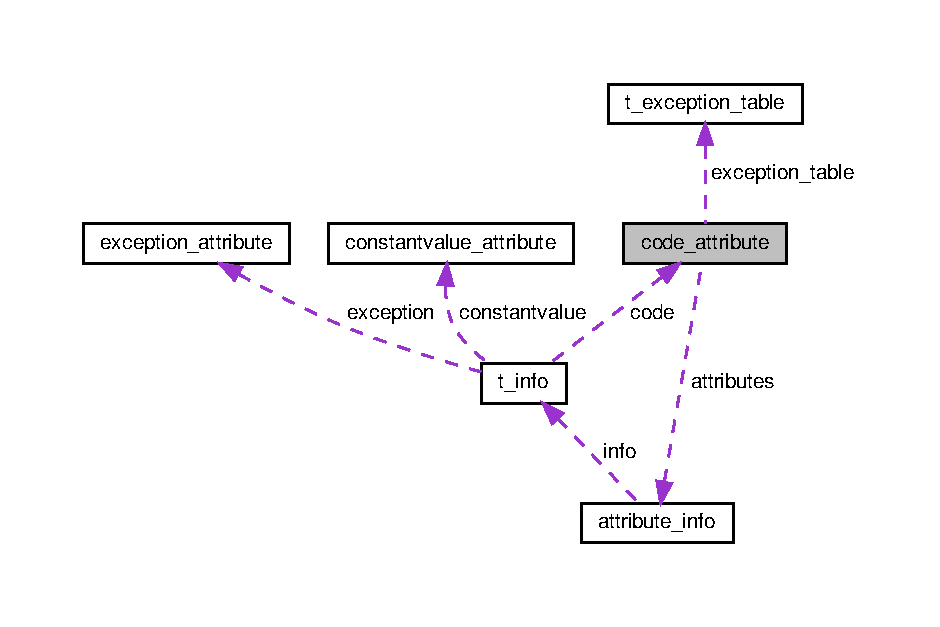
\includegraphics[width=350pt]{structcode__attribute__coll__graph}
\end{center}
\end{figure}
\subsection*{Campos de Dados}
\begin{DoxyCompactItemize}
\item 
\mbox{\Hypertarget{structcode__attribute_ad8f0d9ec65c9065df510fb7313133eb0}\label{structcode__attribute_ad8f0d9ec65c9065df510fb7313133eb0}} 
unsigned short {\bfseries max\+\_\+stack}
\item 
\mbox{\Hypertarget{structcode__attribute_aa5c39f7692d14498f497ac2425595dda}\label{structcode__attribute_aa5c39f7692d14498f497ac2425595dda}} 
unsigned short {\bfseries max\+\_\+locals}
\item 
\mbox{\Hypertarget{structcode__attribute_a8d9bb88d00f7285dbad08ec687adfd2c}\label{structcode__attribute_a8d9bb88d00f7285dbad08ec687adfd2c}} 
unsigned int {\bfseries code\+\_\+length}
\item 
\mbox{\Hypertarget{structcode__attribute_ad469a918dcfae54358813c9ccfa2b603}\label{structcode__attribute_ad469a918dcfae54358813c9ccfa2b603}} 
unsigned char $\ast$ {\bfseries code}
\item 
\mbox{\Hypertarget{structcode__attribute_a52263ac885da86196b36a51e7ee5bd6e}\label{structcode__attribute_a52263ac885da86196b36a51e7ee5bd6e}} 
unsigned short {\bfseries exception\+\_\+table\+\_\+length}
\item 
\mbox{\Hypertarget{structcode__attribute_a7d1657d4edf179c1596f9c102a887b3e}\label{structcode__attribute_a7d1657d4edf179c1596f9c102a887b3e}} 
\hyperlink{structt__exception__table}{t\+\_\+exception\+\_\+table} $\ast$$\ast$ {\bfseries exception\+\_\+table}
\item 
\mbox{\Hypertarget{structcode__attribute_af71546c75dc3185e14b8cd5eb8cd6a24}\label{structcode__attribute_af71546c75dc3185e14b8cd5eb8cd6a24}} 
unsigned short {\bfseries attribute\+\_\+count}
\item 
\mbox{\Hypertarget{structcode__attribute_a9f45491da8c177e471b75c9539bb37b2}\label{structcode__attribute_a9f45491da8c177e471b75c9539bb37b2}} 
\hyperlink{structattribute__info}{attribute\+\_\+info} $\ast$ {\bfseries attributes}
\end{DoxyCompactItemize}


\subsection{Descrição detalhada}
Estrutura de dados para salvar atributos do tipo code. 

Estrutura de dados para salvar atributos de tipo \char`\"{}exception\char`\"{}. 

A documentação para esta estrutura foi gerada a partir do seguinte ficheiro\+:\begin{DoxyCompactItemize}
\item 
include/\hyperlink{attributes_8h}{attributes.\+h}\end{DoxyCompactItemize}

\hypertarget{structconstantvalue__attribute}{}\section{Referência à estrutura constantvalue\+\_\+attribute}
\label{structconstantvalue__attribute}\index{constantvalue\+\_\+attribute@{constantvalue\+\_\+attribute}}


Struct para carregar o index dos atributos da \char`\"{}constantpool\char`\"{}.  




{\ttfamily \#include $<$attributes.\+h$>$}

\subsection*{Campos de Dados}
\begin{DoxyCompactItemize}
\item 
\mbox{\Hypertarget{structconstantvalue__attribute_ad58e1db4120139c8be419ec651ab3fc9}\label{structconstantvalue__attribute_ad58e1db4120139c8be419ec651ab3fc9}} 
unsigned short {\bfseries constantvalue\+\_\+index}
\end{DoxyCompactItemize}


\subsection{Descrição detalhada}
Struct para carregar o index dos atributos da \char`\"{}constantpool\char`\"{}. 

A documentação para esta estrutura foi gerada a partir do seguinte ficheiro\+:\begin{DoxyCompactItemize}
\item 
include/\hyperlink{attributes_8h}{attributes.\+h}\end{DoxyCompactItemize}

\hypertarget{structcp__info}{}\section{Referência à estrutura cp\+\_\+info}
\label{structcp__info}\index{cp\+\_\+info@{cp\+\_\+info}}


Possui um elemento pool de constante.  




{\ttfamily \#include $<$constant\+Pool.\+h$>$}



Diagrama de colaboração para cp\+\_\+info\+:\nopagebreak
\begin{figure}[H]
\begin{center}
\leavevmode
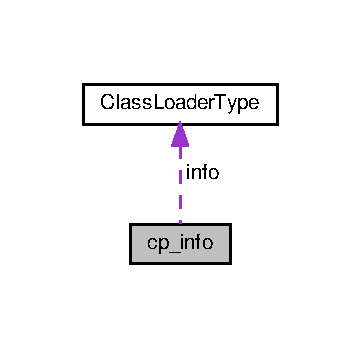
\includegraphics[width=173pt]{structcp__info__coll__graph}
\end{center}
\end{figure}
\subsection*{Campos de Dados}
\begin{DoxyCompactItemize}
\item 
\mbox{\Hypertarget{structcp__info_a850b66fa196e9fc2e898ca41d558e248}\label{structcp__info_a850b66fa196e9fc2e898ca41d558e248}} 
U1 {\bfseries tag}
\item 
\mbox{\Hypertarget{structcp__info_aafa07de27e22632ed56ab8fbffbe2559}\label{structcp__info_aafa07de27e22632ed56ab8fbffbe2559}} 
\hyperlink{unionClassLoaderType}{Class\+Loader\+Type} $\ast$ {\bfseries info}
\end{DoxyCompactItemize}


\subsection{Descrição detalhada}
Possui um elemento pool de constante. 

A documentação para esta estrutura foi gerada a partir do seguinte ficheiro\+:\begin{DoxyCompactItemize}
\item 
include/\hyperlink{constantPool_8h}{constant\+Pool.\+h}\end{DoxyCompactItemize}

\hypertarget{unionelement__u}{}\section{Referência à união element\+\_\+u}
\label{unionelement__u}\index{element\+\_\+u@{element\+\_\+u}}


Generalização de funções de retorno/input Union responsável pela generalização de funções de retorno e uma função de input.  




{\ttfamily \#include $<$base\+Types.\+h$>$}

\subsection*{Campos de Dados}
\begin{DoxyCompactItemize}
\item 
\mbox{\Hypertarget{unionelement__u_a055cfbd7f84724337a2cb16acdedab90}\label{unionelement__u_a055cfbd7f84724337a2cb16acdedab90}} 
double {\bfseries d}
\item 
\mbox{\Hypertarget{unionelement__u_ad3caae754d93e7fa606a0756f5ddc6a6}\label{unionelement__u_ad3caae754d93e7fa606a0756f5ddc6a6}} 
float {\bfseries f}
\item 
\mbox{\Hypertarget{unionelement__u_ac1564bf5b02b69382469449ba266dc9a}\label{unionelement__u_ac1564bf5b02b69382469449ba266dc9a}} 
uint32\+\_\+t {\bfseries i}
\item 
\mbox{\Hypertarget{unionelement__u_a8230539b3b28f57ac3fd61e10c76a740}\label{unionelement__u_a8230539b3b28f57ac3fd61e10c76a740}} 
int32\+\_\+t {\bfseries is}
\item 
\mbox{\Hypertarget{unionelement__u_aca3c96df160bc775791470b98e15710f}\label{unionelement__u_aca3c96df160bc775791470b98e15710f}} 
uint64\+\_\+t {\bfseries l}
\item 
\mbox{\Hypertarget{unionelement__u_af52b13fa38bfc4e5a98d4b868324ee27}\label{unionelement__u_af52b13fa38bfc4e5a98d4b868324ee27}} 
int64\+\_\+t {\bfseries ls}
\item 
\mbox{\Hypertarget{unionelement__u_a85c036f57770aeab7ed90947ffdfda53}\label{unionelement__u_a85c036f57770aeab7ed90947ffdfda53}} 
uint16\+\_\+t {\bfseries s}
\item 
\mbox{\Hypertarget{unionelement__u_ab90ee55202fd11a2dc3cf48c74e55dab}\label{unionelement__u_ab90ee55202fd11a2dc3cf48c74e55dab}} 
int16\+\_\+t {\bfseries ss}
\item 
\mbox{\Hypertarget{unionelement__u_a53d82c8469f011fdb1e35f88738aaf5e}\label{unionelement__u_a53d82c8469f011fdb1e35f88738aaf5e}} 
uint8\+\_\+t {\bfseries b}
\item 
\mbox{\Hypertarget{unionelement__u_ae2cf2a77222a37a817fba0e70266ddf6}\label{unionelement__u_ae2cf2a77222a37a817fba0e70266ddf6}} 
int8\+\_\+t {\bfseries bs}
\item 
\mbox{\Hypertarget{unionelement__u_a3c7acdaf4dc01ef8694967376100fc8f}\label{unionelement__u_a3c7acdaf4dc01ef8694967376100fc8f}} 
int $\ast$ {\bfseries pi}
\end{DoxyCompactItemize}


\subsection{Descrição detalhada}
Generalização de funções de retorno/input Union responsável pela generalização de funções de retorno e uma função de input. 

A documentação para esta união foi gerada a partir do seguinte ficheiro\+:\begin{DoxyCompactItemize}
\item 
include/\hyperlink{baseTypes_8h}{base\+Types.\+h}\end{DoxyCompactItemize}

\hypertarget{structexception__attribute}{}\section{Referência à estrutura exception\+\_\+attribute}
\label{structexception__attribute}\index{exception\+\_\+attribute@{exception\+\_\+attribute}}
\subsection*{Campos de Dados}
\begin{DoxyCompactItemize}
\item 
\mbox{\Hypertarget{structexception__attribute_a40daaffb1cea794d6b65513bc7639d88}\label{structexception__attribute_a40daaffb1cea794d6b65513bc7639d88}} 
unsigned short {\bfseries number\+\_\+of\+\_\+exceptions}
\item 
\mbox{\Hypertarget{structexception__attribute_a017de83073154b04633ebe00dfb77932}\label{structexception__attribute_a017de83073154b04633ebe00dfb77932}} 
unsigned short $\ast$ {\bfseries exception\+\_\+index\+\_\+table}
\end{DoxyCompactItemize}


A documentação para esta estrutura foi gerada a partir do seguinte ficheiro\+:\begin{DoxyCompactItemize}
\item 
include/\hyperlink{attributes_8h}{attributes.\+h}\end{DoxyCompactItemize}

\hypertarget{structfield__info}{}\section{Referência à estrutura field\+\_\+info}
\label{structfield__info}\index{field\+\_\+info@{field\+\_\+info}}


Struct de armazenamento.  




{\ttfamily \#include $<$fields.\+h$>$}



Diagrama de colaboração para field\+\_\+info\+:\nopagebreak
\begin{figure}[H]
\begin{center}
\leavevmode
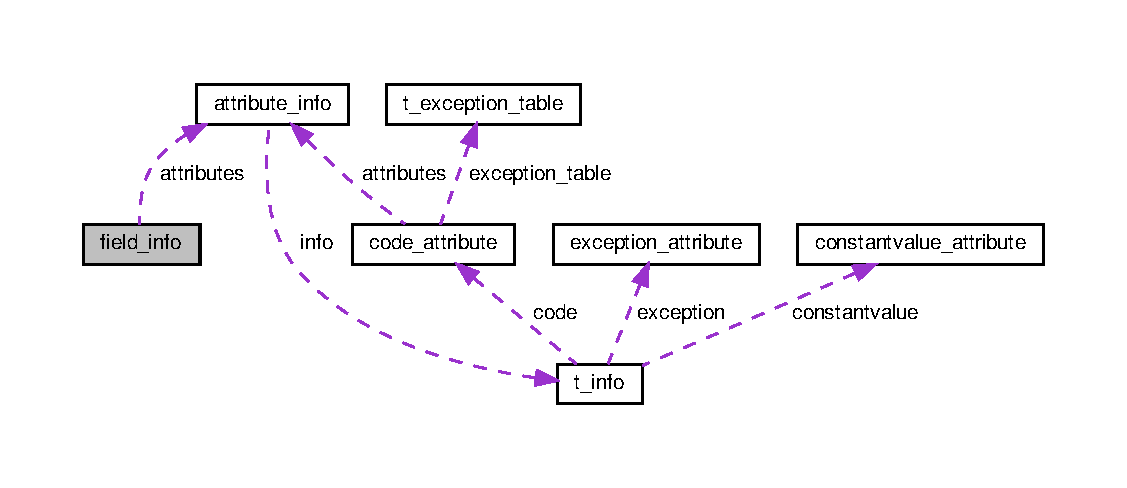
\includegraphics[width=350pt]{structfield__info__coll__graph}
\end{center}
\end{figure}
\subsection*{Campos de Dados}
\begin{DoxyCompactItemize}
\item 
\mbox{\Hypertarget{structfield__info_a52647ac149308d5ef9f010689400ee4c}\label{structfield__info_a52647ac149308d5ef9f010689400ee4c}} 
unsigned char {\bfseries access\+Flags}
\item 
\mbox{\Hypertarget{structfield__info_abb3389c726c0efe891c2d26567ecea49}\label{structfield__info_abb3389c726c0efe891c2d26567ecea49}} 
unsigned char {\bfseries name\+\_\+index}
\item 
\mbox{\Hypertarget{structfield__info_afe39e4e9e594dfce15635923ad7d1f06}\label{structfield__info_afe39e4e9e594dfce15635923ad7d1f06}} 
unsigned char {\bfseries descriptor\+\_\+index}
\item 
\mbox{\Hypertarget{structfield__info_a89ea1703d384244c336899c3b04850f9}\label{structfield__info_a89ea1703d384244c336899c3b04850f9}} 
unsigned char {\bfseries attributes\+\_\+count}
\item 
\mbox{\Hypertarget{structfield__info_afdda114944ae5eaae78c237f99257108}\label{structfield__info_afdda114944ae5eaae78c237f99257108}} 
\hyperlink{structattribute__info}{attribute\+\_\+info} $\ast$ {\bfseries attributes}
\end{DoxyCompactItemize}


\subsection{Descrição detalhada}
Struct de armazenamento. 

Struct responsável por armazenar os campos declarados. 

A documentação para esta estrutura foi gerada a partir do seguinte ficheiro\+:\begin{DoxyCompactItemize}
\item 
include/\hyperlink{fields_8h}{fields.\+h}\end{DoxyCompactItemize}

\hypertarget{structframe__s}{}\section{Referência à estrutura frame\+\_\+s}
\label{structframe__s}\index{frame\+\_\+s@{frame\+\_\+s}}


Estrutura de armazenamento.  




{\ttfamily \#include $<$frame.\+h$>$}



Diagrama de colaboração para frame\+\_\+s\+:
\nopagebreak
\begin{figure}[H]
\begin{center}
\leavevmode
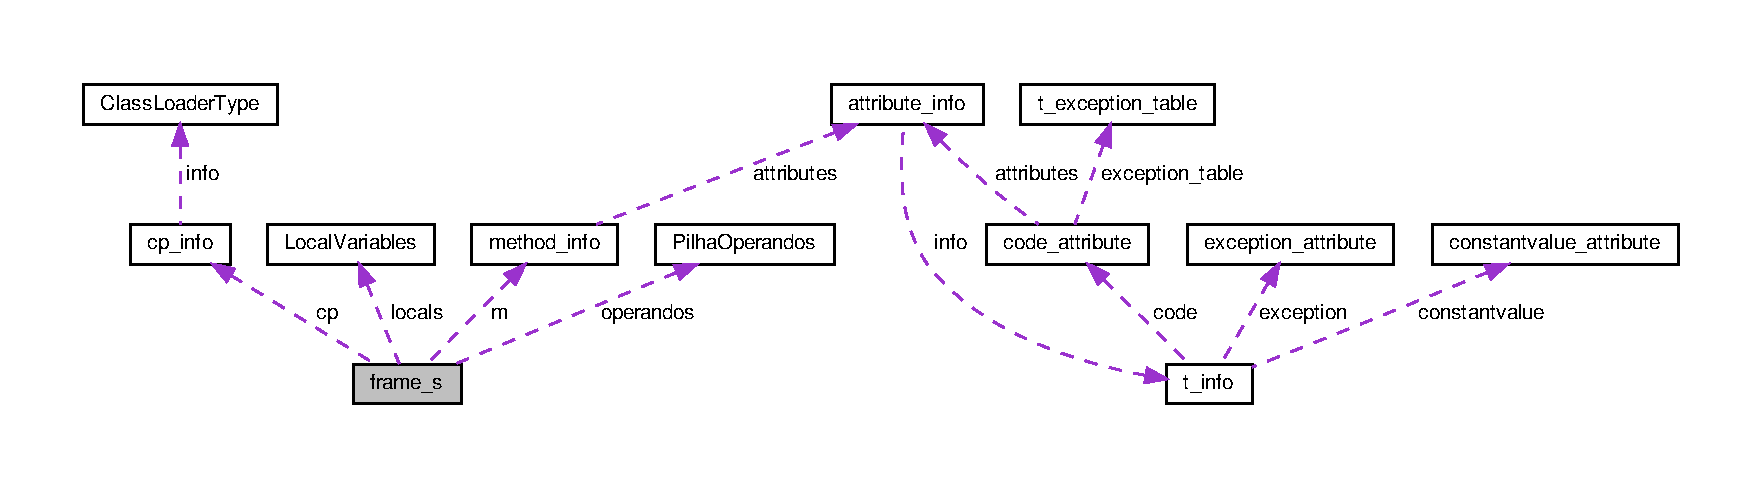
\includegraphics[width=350pt]{structframe__s__coll__graph}
\end{center}
\end{figure}
\subsection*{Campos de Dados}
\begin{DoxyCompactItemize}
\item 
\mbox{\Hypertarget{structframe__s_a74703c716b34b0be42af1c698ef9f621}\label{structframe__s_a74703c716b34b0be42af1c698ef9f621}} 
unsigned char $\ast$ {\bfseries pc}
\item 
\mbox{\Hypertarget{structframe__s_a9e281d20d1a4393e4744dd1d07de5126}\label{structframe__s_a9e281d20d1a4393e4744dd1d07de5126}} 
\hyperlink{structcp__info}{cp\+\_\+info} $\ast$ {\bfseries cp}
\item 
\mbox{\Hypertarget{structframe__s_a5377bbe53d53c855f8e11544cb26c9d2}\label{structframe__s_a5377bbe53d53c855f8e11544cb26c9d2}} 
\hyperlink{classPilhaOperandos}{Pilha\+Operandos} $\ast$ {\bfseries operandos}
\item 
\mbox{\Hypertarget{structframe__s_a4c0fe214398d7c0b688465bbed8a36d1}\label{structframe__s_a4c0fe214398d7c0b688465bbed8a36d1}} 
\hyperlink{classLocalVariables}{Local\+Variables} $\ast$ {\bfseries locals}
\item 
\mbox{\Hypertarget{structframe__s_aa771844a4dc507d1c37bfb5b378889e3}\label{structframe__s_aa771844a4dc507d1c37bfb5b378889e3}} 
\hyperlink{structmethod__info}{method\+\_\+info} {\bfseries m}
\end{DoxyCompactItemize}


\subsection{Descrição detalhada}
Estrutura de armazenamento. 

Responsável por todas as informações necessárias para a execução de um método. 

A documentação para esta estrutura foi gerada a partir do seguinte ficheiro\+:\begin{DoxyCompactItemize}
\item 
include/\hyperlink{frame_8h}{frame.\+h}\end{DoxyCompactItemize}

\hypertarget{classFrameStack}{}\section{Referência à classe Frame\+Stack}
\label{classFrameStack}\index{Frame\+Stack@{Frame\+Stack}}


Classe de pilha de frames.  




{\ttfamily \#include $<$frame.\+h$>$}

\subsection*{Membros públicos}
\begin{DoxyCompactItemize}
\item 
\hyperlink{classFrameStack_aaa727d2a58e24e6f02f1cd358a804981}{Frame\+Stack} (\hyperlink{classLeitor}{Leitor} $\ast$)
\begin{DoxyCompactList}\small\item\em Contrutor da pilha de frame. \end{DoxyCompactList}\item 
void \hyperlink{classFrameStack_af06f3e125bea380e017afd14fb6b14a3}{set\+Arguments} (std\+::vector$<$ \hyperlink{structtypedElement__s}{typed\+Element} $>$)
\begin{DoxyCompactList}\small\item\em Configura os argumentos. \end{DoxyCompactList}\item 
\mbox{\Hypertarget{classFrameStack_a9ad510705082a0055eb03e9cbea295f3}\label{classFrameStack_a9ad510705082a0055eb03e9cbea295f3}} 
void \hyperlink{classFrameStack_a9ad510705082a0055eb03e9cbea295f3}{execute} ()
\begin{DoxyCompactList}\small\item\em Executa o método atual e os métodos chamados. \end{DoxyCompactList}\item 
void \hyperlink{classFrameStack_aefe44d87f18ddf549ca64416569f7a40}{add\+Frame} (\hyperlink{structmethod__info}{method\+\_\+info}, \hyperlink{structcp__info}{cp\+\_\+info} $\ast$)
\begin{DoxyCompactList}\small\item\em Adiciona um frame no topo da pilha. \end{DoxyCompactList}\item 
\mbox{\Hypertarget{classFrameStack_a84bdb9bfff23f213df4948bcba469a89}\label{classFrameStack_a84bdb9bfff23f213df4948bcba469a89}} 
void {\bfseries add\+Frame} (\hyperlink{structmethod__info}{method\+\_\+info} $\ast$, \hyperlink{structcp__info}{cp\+\_\+info} $\ast$)
\item 
\mbox{\Hypertarget{classFrameStack_a7da31bde9fe2f7cf6a4e2497445223a5}\label{classFrameStack_a7da31bde9fe2f7cf6a4e2497445223a5}} 
void \hyperlink{classFrameStack_a7da31bde9fe2f7cf6a4e2497445223a5}{pop} ()
\begin{DoxyCompactList}\small\item\em Dá um pop no método atual. \end{DoxyCompactList}\end{DoxyCompactItemize}


\subsection{Descrição detalhada}
Classe de pilha de frames. 

Responsável por todas as operações que usam o frame. 

\subsection{Documentação dos Construtores \& Destrutor}
\mbox{\Hypertarget{classFrameStack_aaa727d2a58e24e6f02f1cd358a804981}\label{classFrameStack_aaa727d2a58e24e6f02f1cd358a804981}} 
\index{Frame\+Stack@{Frame\+Stack}!Frame\+Stack@{Frame\+Stack}}
\index{Frame\+Stack@{Frame\+Stack}!Frame\+Stack@{Frame\+Stack}}
\subsubsection{\texorpdfstring{Frame\+Stack()}{FrameStack()}}
{\footnotesize\ttfamily Frame\+Stack\+::\+Frame\+Stack (\begin{DoxyParamCaption}\item[{\hyperlink{classLeitor}{Leitor} $\ast$}]{l }\end{DoxyParamCaption})}



Contrutor da pilha de frame. 


\begin{DoxyParams}{Parâmetros}
{\em l} & O que é lido do arquivo .class. \\
\hline
\end{DoxyParams}


\subsection{Documentação dos métodos}
\mbox{\Hypertarget{classFrameStack_aefe44d87f18ddf549ca64416569f7a40}\label{classFrameStack_aefe44d87f18ddf549ca64416569f7a40}} 
\index{Frame\+Stack@{Frame\+Stack}!add\+Frame@{add\+Frame}}
\index{add\+Frame@{add\+Frame}!Frame\+Stack@{Frame\+Stack}}
\subsubsection{\texorpdfstring{add\+Frame()}{addFrame()}}
{\footnotesize\ttfamily void Frame\+Stack\+::add\+Frame (\begin{DoxyParamCaption}\item[{\hyperlink{structmethod__info}{method\+\_\+info}}]{m,  }\item[{\hyperlink{structcp__info}{cp\+\_\+info} $\ast$}]{cp }\end{DoxyParamCaption})}



Adiciona um frame no topo da pilha. 


\begin{DoxyParams}{Parâmetros}
{\em m} & Método no qual o frame será criado. \\
\hline
{\em cp} & Um ponteiro para o pool de constantes.\\
\hline
{\em m} & Ponteiro para o método no qual o frame será criado. \\
\hline
{\em cp} & Um ponteiro para o pool de constantes. \\
\hline
\end{DoxyParams}
\mbox{\Hypertarget{classFrameStack_af06f3e125bea380e017afd14fb6b14a3}\label{classFrameStack_af06f3e125bea380e017afd14fb6b14a3}} 
\index{Frame\+Stack@{Frame\+Stack}!set\+Arguments@{set\+Arguments}}
\index{set\+Arguments@{set\+Arguments}!Frame\+Stack@{Frame\+Stack}}
\subsubsection{\texorpdfstring{set\+Arguments()}{setArguments()}}
{\footnotesize\ttfamily void Frame\+Stack\+::set\+Arguments (\begin{DoxyParamCaption}\item[{std\+::vector$<$ \hyperlink{structtypedElement__s}{typed\+Element} $>$}]{param }\end{DoxyParamCaption})}



Configura os argumentos. 


\begin{DoxyParams}{Parâmetros}
{\em Vetor} & com os argumentos a serem copiados para o vetor de variáveis locais \\
\hline
\end{DoxyParams}


A documentação para esta classe foi gerada a partir dos seguintes ficheiros\+:\begin{DoxyCompactItemize}
\item 
include/\hyperlink{frame_8h}{frame.\+h}\item 
src/\hyperlink{frame_8cpp}{frame.\+cpp}\end{DoxyCompactItemize}

\hypertarget{classHeap}{}\section{Referência à classe Heap}
\label{classHeap}\index{Heap@{Heap}}


Classe do heap.  




{\ttfamily \#include $<$heap.\+h$>$}

\subsection*{Membros públicos estáticos}
\begin{DoxyCompactItemize}
\item 
static void \hyperlink{classHeap_a91b503526ad198b5590ed4a787d4f3d2}{add\+Object} (\hyperlink{classClasseInstancia}{Classe\+Instancia} $\ast$)
\begin{DoxyCompactList}\small\item\em Adiciona novo objeto no heap. \end{DoxyCompactList}\end{DoxyCompactItemize}


\subsection{Descrição detalhada}
Classe do heap. 

Gerencia as operações do heap. 

\subsection{Documentação dos métodos}
\mbox{\Hypertarget{classHeap_a91b503526ad198b5590ed4a787d4f3d2}\label{classHeap_a91b503526ad198b5590ed4a787d4f3d2}} 
\index{Heap@{Heap}!add\+Object@{add\+Object}}
\index{add\+Object@{add\+Object}!Heap@{Heap}}
\subsubsection{\texorpdfstring{add\+Object()}{addObject()}}
{\footnotesize\ttfamily static void Heap\+::add\+Object (\begin{DoxyParamCaption}\item[{\hyperlink{classClasseInstancia}{Classe\+Instancia} $\ast$}]{ci }\end{DoxyParamCaption})\hspace{0.3cm}{\ttfamily [static]}}



Adiciona novo objeto no heap. 


\begin{DoxyParams}{Parâmetros}
{\em ci} & -\/ ponteiro para o novo objeto. \\
\hline
\end{DoxyParams}


A documentação para esta classe foi gerada a partir dos seguintes ficheiros\+:\begin{DoxyCompactItemize}
\item 
include/\hyperlink{heap_8h}{heap.\+h}\item 
src/\hyperlink{heap_8cpp}{heap.\+cpp}\end{DoxyCompactItemize}

\hypertarget{classLeitor}{}\section{Referência à classe Leitor}
\label{classLeitor}\index{Leitor@{Leitor}}
\subsection*{Membros públicos}
\begin{DoxyCompactItemize}
\item 
\hyperlink{classLeitor_a0a1e8b666d75c2fd2c112affc0a8f55a}{Leitor} (char $\ast$in)
\item 
\hyperlink{classLeitor_a0ab1016df547c6e5081607b916eb7825}{Leitor} (std\+::string in)
\item 
int \hyperlink{classLeitor_a82a5ba05f6445e0c56f15eddecef21a3}{run} ()
\begin{DoxyCompactList}\small\item\em Carrega todas as informções do class file e as imprime. \end{DoxyCompactList}\item 
int \hyperlink{classLeitor_a69b1505dbce4cfdbb9fcb7e70ca639e6}{load} ()
\begin{DoxyCompactList}\small\item\em Carrega todas as informações do class file. \end{DoxyCompactList}\item 
void \hyperlink{classLeitor_a61890be2d648f47fcc6817ac8c751660}{print\+General\+Information} ()
\begin{DoxyCompactList}\small\item\em Imprime informações gerais do .class. \end{DoxyCompactList}\item 
bool \hyperlink{classLeitor_a1f50a340fba40d773af019975a3ab385}{show} ()
\begin{DoxyCompactList}\small\item\em Imprime todas as informações do .class. \end{DoxyCompactList}\item 
bool \hyperlink{classLeitor_a64ccb4aca8b2c665b79ace09a3423b77}{valid\+Extension} ()
\begin{DoxyCompactList}\small\item\em Verifica se a extensão do arquivo é .class. \end{DoxyCompactList}\item 
bool \hyperlink{classLeitor_a737ca7d70af56cab2c01fbfca0c774f7}{has\+Main} ()
\begin{DoxyCompactList}\small\item\em Verifica se o .class possui função main. \end{DoxyCompactList}\item 
\hyperlink{structmethod__info}{method\+\_\+info} \hyperlink{classLeitor_a462716ecacea891a2e07e77eec0dabe7}{get\+Main} ()
\begin{DoxyCompactList}\small\item\em Retorna o método main. \end{DoxyCompactList}\item 
bool \hyperlink{classLeitor_a31934be87590ff3732b3117ebe96cc34}{has\+Clinit} ()
\begin{DoxyCompactList}\small\item\em Verifica se o .class tem o método $<$clinit$>$ \end{DoxyCompactList}\item 
\hyperlink{structmethod__info}{method\+\_\+info} \hyperlink{classLeitor_a4c64b307c9690ba25f04e911e07fe5a3}{get\+Clinit} ()
\begin{DoxyCompactList}\small\item\em Retorna o método $<$clinit$>$ \end{DoxyCompactList}\item 
bool \hyperlink{classLeitor_a46501dcb0e924524b6354f5459503ce8}{check\+This\+Class} ()
\begin{DoxyCompactList}\small\item\em Verifica se a class definida é igual ao nome da classe sem extensões. \end{DoxyCompactList}\item 
int \hyperlink{classLeitor_a55c4c9df6771ce70388001a064f28256}{get\+Status} ()
\begin{DoxyCompactList}\small\item\em Retorna o status lido, informando para o método que chamou o que aconteceu. \end{DoxyCompactList}\item 
\hyperlink{structcp__info}{cp\+\_\+info} $\ast$ \hyperlink{classLeitor_a95bd2e9979122b1d742ce2e0dd6c4a4b}{get\+CP} () const
\begin{DoxyCompactList}\small\item\em Retorna referencia a constant pool. \end{DoxyCompactList}\item 
U2 \hyperlink{classLeitor_a53b7aac0c6d2b75104c6d53abd23b37e}{get\+Length\+CP} ()
\begin{DoxyCompactList}\small\item\em Retorna o valor do tamanho da constant pool. \end{DoxyCompactList}\item 
char $\ast$ \hyperlink{classLeitor_a28757ad7042926102520d2f28387acfe}{get\+Path} ()
\begin{DoxyCompactList}\small\item\em Pega o caminho do arquivo .class. \end{DoxyCompactList}\item 
\hyperlink{structmethod__info}{method\+\_\+info} $\ast$ \hyperlink{classLeitor_aa08c48544276f3c849eb138576d9f1b3}{get\+Methods} ()
\begin{DoxyCompactList}\small\item\em Retorna todos os métodos. \end{DoxyCompactList}\item 
U2 \hyperlink{classLeitor_a1bf5bcc94ae930802de39077836d6566}{get\+Methods\+Count} ()
\begin{DoxyCompactList}\small\item\em Retorna o numero de methods. \end{DoxyCompactList}\item 
U2 \hyperlink{classLeitor_a96d06888c1e8d4a6516c5e5f36d49801}{get\+This\+\_\+class} ()
\begin{DoxyCompactList}\small\item\em Retorna um índice da constant pool que aponta para string com nome da class. \end{DoxyCompactList}\item 
U2 \hyperlink{classLeitor_ab70e078103dc971808b62ab08cbfb4fa}{get\+Super\+\_\+class} ()
\begin{DoxyCompactList}\small\item\em Retorna um índice da constant pool que aponta para string com nome da superclass. \end{DoxyCompactList}\item 
U2 \hyperlink{classLeitor_a59287cad03c19ca411b7befce0008870}{get\+Fields\+Count} ()
\begin{DoxyCompactList}\small\item\em Retorna número de fields. \end{DoxyCompactList}\item 
\hyperlink{structfield__info}{field\+\_\+info} $\ast$ \hyperlink{classLeitor_a32f5a9515e24523f3f4016141de5cc9d}{get\+Fields} ()
\begin{DoxyCompactList}\small\item\em Retorna todos os fields. \end{DoxyCompactList}\item 
\hyperlink{structfield__info}{field\+\_\+info} $\ast$ \hyperlink{classLeitor_a1c0eb678858e00efa9c18d63832d3dff}{get\+Field} (string field\+\_\+name)
\begin{DoxyCompactList}\small\item\em Retorna um field. \end{DoxyCompactList}\item 
\hyperlink{structmethod__info}{method\+\_\+info} $\ast$ \hyperlink{classLeitor_a721a60b281566287c7845c52a667ecc1}{get\+Method} (string name, string descriptor)
\begin{DoxyCompactList}\small\item\em Retorna o method info. \end{DoxyCompactList}\item 
\hyperlink{classLeitor}{Leitor} $\ast$ \hyperlink{classLeitor_a568b259f176676472196ad0fb127c4f2}{get\+Class\+That\+Has\+Serached\+Method} (string name, string descriptor)
\begin{DoxyCompactList}\small\item\em Retorna o ponteiro para o leitor do .class que contém o método encontrado em get\+Method. \end{DoxyCompactList}\end{DoxyCompactItemize}


\subsection{Documentação dos Construtores \& Destrutor}
\mbox{\Hypertarget{classLeitor_a0a1e8b666d75c2fd2c112affc0a8f55a}\label{classLeitor_a0a1e8b666d75c2fd2c112affc0a8f55a}} 
\index{Leitor@{Leitor}!Leitor@{Leitor}}
\index{Leitor@{Leitor}!Leitor@{Leitor}}
\subsubsection{\texorpdfstring{Leitor()}{Leitor()}\hspace{0.1cm}{\footnotesize\ttfamily [1/2]}}
{\footnotesize\ttfamily Leitor\+::\+Leitor (\begin{DoxyParamCaption}\item[{char $\ast$}]{in }\end{DoxyParamCaption})}

Construtor que configura um objeto da classe \hyperlink{classLeitor}{Leitor} com o nome do arquivo passado.


\begin{DoxyParams}{Parâmetros}
{\em in} & argumento passado como nome do arquivo na inicializacao do programa \\
\hline
\end{DoxyParams}
\mbox{\Hypertarget{classLeitor_a0ab1016df547c6e5081607b916eb7825}\label{classLeitor_a0ab1016df547c6e5081607b916eb7825}} 
\index{Leitor@{Leitor}!Leitor@{Leitor}}
\index{Leitor@{Leitor}!Leitor@{Leitor}}
\subsubsection{\texorpdfstring{Leitor()}{Leitor()}\hspace{0.1cm}{\footnotesize\ttfamily [2/2]}}
{\footnotesize\ttfamily Leitor\+::\+Leitor (\begin{DoxyParamCaption}\item[{std\+::string}]{in }\end{DoxyParamCaption})}

Construtor que configura um objeto da classe \hyperlink{classLeitor}{Leitor} com o nome do arquivo passado.


\begin{DoxyParams}{Parâmetros}
{\em in} & argumento passado como nome do arquivo na inicializacao do programa \\
\hline
\end{DoxyParams}


\subsection{Documentação dos métodos}
\mbox{\Hypertarget{classLeitor_a46501dcb0e924524b6354f5459503ce8}\label{classLeitor_a46501dcb0e924524b6354f5459503ce8}} 
\index{Leitor@{Leitor}!check\+This\+Class@{check\+This\+Class}}
\index{check\+This\+Class@{check\+This\+Class}!Leitor@{Leitor}}
\subsubsection{\texorpdfstring{check\+This\+Class()}{checkThisClass()}}
{\footnotesize\ttfamily bool Leitor\+::check\+This\+Class (\begin{DoxyParamCaption}{ }\end{DoxyParamCaption})}



Verifica se a class definida é igual ao nome da classe sem extensões. 

Verifica se a .class lida no bytecode é a mesma que foi declarada no nome do arquivo \begin{DoxyReturn}{Retorna}
booleano indicando se a .class está correta 
\end{DoxyReturn}
\mbox{\Hypertarget{classLeitor_a568b259f176676472196ad0fb127c4f2}\label{classLeitor_a568b259f176676472196ad0fb127c4f2}} 
\index{Leitor@{Leitor}!get\+Class\+That\+Has\+Serached\+Method@{get\+Class\+That\+Has\+Serached\+Method}}
\index{get\+Class\+That\+Has\+Serached\+Method@{get\+Class\+That\+Has\+Serached\+Method}!Leitor@{Leitor}}
\subsubsection{\texorpdfstring{get\+Class\+That\+Has\+Serached\+Method()}{getClassThatHasSerachedMethod()}}
{\footnotesize\ttfamily U2 Leitor\+::get\+Class\+That\+Has\+Serached\+Method (\begin{DoxyParamCaption}\item[{string}]{name,  }\item[{string}]{descriptor }\end{DoxyParamCaption})}



Retorna o ponteiro para o leitor do .class que contém o método encontrado em get\+Method. 

Retorna a classe do metodo que esta sendo procurado 
\begin{DoxyParams}{Parâmetros}
{\em name} & nome do method \\
\hline
{\em descriptor} & descritor do method \\
\hline
\end{DoxyParams}
\begin{DoxyReturn}{Retorna}
classe \hyperlink{classLeitor}{Leitor}
\end{DoxyReturn}

\begin{DoxyParams}{Parâmetros}
{\em name} & Nome do method desejado \\
\hline
{\em descriptor} & Descritor do method desejado \\
\hline
\end{DoxyParams}
\mbox{\Hypertarget{classLeitor_a4c64b307c9690ba25f04e911e07fe5a3}\label{classLeitor_a4c64b307c9690ba25f04e911e07fe5a3}} 
\index{Leitor@{Leitor}!get\+Clinit@{get\+Clinit}}
\index{get\+Clinit@{get\+Clinit}!Leitor@{Leitor}}
\subsubsection{\texorpdfstring{get\+Clinit()}{getClinit()}}
{\footnotesize\ttfamily \hyperlink{structmethod__info}{method\+\_\+info} Leitor\+::get\+Clinit (\begin{DoxyParamCaption}{ }\end{DoxyParamCaption})}



Retorna o método $<$clinit$>$ 

Retorna o metodo clinit no formato da struct \hyperlink{structmethod__info}{method\+\_\+info} \begin{DoxyReturn}{Retorna}
struct \hyperlink{structmethod__info}{method\+\_\+info} contendo informações sobre o método 
\end{DoxyReturn}
\mbox{\Hypertarget{classLeitor_a95bd2e9979122b1d742ce2e0dd6c4a4b}\label{classLeitor_a95bd2e9979122b1d742ce2e0dd6c4a4b}} 
\index{Leitor@{Leitor}!get\+CP@{get\+CP}}
\index{get\+CP@{get\+CP}!Leitor@{Leitor}}
\subsubsection{\texorpdfstring{get\+C\+P()}{getCP()}}
{\footnotesize\ttfamily \hyperlink{structcp__info}{cp\+\_\+info} $\ast$ Leitor\+::get\+CP (\begin{DoxyParamCaption}{ }\end{DoxyParamCaption}) const}



Retorna referencia a constant pool. 

método para pegar a constant pool lida \begin{DoxyReturn}{Retorna}
Retorna a array com a constant pool 
\end{DoxyReturn}
\mbox{\Hypertarget{classLeitor_a1c0eb678858e00efa9c18d63832d3dff}\label{classLeitor_a1c0eb678858e00efa9c18d63832d3dff}} 
\index{Leitor@{Leitor}!get\+Field@{get\+Field}}
\index{get\+Field@{get\+Field}!Leitor@{Leitor}}
\subsubsection{\texorpdfstring{get\+Field()}{getField()}}
{\footnotesize\ttfamily U2 Leitor\+::get\+Field (\begin{DoxyParamCaption}\item[{string}]{field\+\_\+name }\end{DoxyParamCaption})}



Retorna um field. 

Retorna um field 
\begin{DoxyParams}{Parâmetros}
{\em field\+\_\+name} & nome do field que deseja retornar \\
\hline
\end{DoxyParams}
\begin{DoxyReturn}{Retorna}
struct \hyperlink{structfield__info}{field\+\_\+info} com a informação da field passada no parâmetro
\end{DoxyReturn}

\begin{DoxyParams}{Parâmetros}
{\em field\+\_\+name} & nome do field desejado \\
\hline
\end{DoxyParams}
\mbox{\Hypertarget{classLeitor_a32f5a9515e24523f3f4016141de5cc9d}\label{classLeitor_a32f5a9515e24523f3f4016141de5cc9d}} 
\index{Leitor@{Leitor}!get\+Fields@{get\+Fields}}
\index{get\+Fields@{get\+Fields}!Leitor@{Leitor}}
\subsubsection{\texorpdfstring{get\+Fields()}{getFields()}}
{\footnotesize\ttfamily U2 Leitor\+::get\+Fields (\begin{DoxyParamCaption}{ }\end{DoxyParamCaption})}



Retorna todos os fields. 

Retorna a array com as fields lidas \begin{DoxyReturn}{Retorna}
a array da struct \hyperlink{structfield__info}{field\+\_\+info} 
\end{DoxyReturn}
\mbox{\Hypertarget{classLeitor_a59287cad03c19ca411b7befce0008870}\label{classLeitor_a59287cad03c19ca411b7befce0008870}} 
\index{Leitor@{Leitor}!get\+Fields\+Count@{get\+Fields\+Count}}
\index{get\+Fields\+Count@{get\+Fields\+Count}!Leitor@{Leitor}}
\subsubsection{\texorpdfstring{get\+Fields\+Count()}{getFieldsCount()}}
{\footnotesize\ttfamily U2 Leitor\+::get\+Fields\+Count (\begin{DoxyParamCaption}{ }\end{DoxyParamCaption})}



Retorna número de fields. 

Retorna o número de fields \begin{DoxyReturn}{Retorna}
uint16\+\_\+t indicando o numero de fields 
\end{DoxyReturn}
\mbox{\Hypertarget{classLeitor_a53b7aac0c6d2b75104c6d53abd23b37e}\label{classLeitor_a53b7aac0c6d2b75104c6d53abd23b37e}} 
\index{Leitor@{Leitor}!get\+Length\+CP@{get\+Length\+CP}}
\index{get\+Length\+CP@{get\+Length\+CP}!Leitor@{Leitor}}
\subsubsection{\texorpdfstring{get\+Length\+C\+P()}{getLengthCP()}}
{\footnotesize\ttfamily U2 Leitor\+::get\+Length\+CP (\begin{DoxyParamCaption}{ }\end{DoxyParamCaption})}



Retorna o valor do tamanho da constant pool. 

método para pegar a constant pool lida \begin{DoxyReturn}{Retorna}
Retorna a array com a constant pool 
\end{DoxyReturn}
\mbox{\Hypertarget{classLeitor_a462716ecacea891a2e07e77eec0dabe7}\label{classLeitor_a462716ecacea891a2e07e77eec0dabe7}} 
\index{Leitor@{Leitor}!get\+Main@{get\+Main}}
\index{get\+Main@{get\+Main}!Leitor@{Leitor}}
\subsubsection{\texorpdfstring{get\+Main()}{getMain()}}
{\footnotesize\ttfamily \hyperlink{structmethod__info}{method\+\_\+info} Leitor\+::get\+Main (\begin{DoxyParamCaption}{ }\end{DoxyParamCaption})}



Retorna o método main. 

Retorna o metodo main no formato da struct \hyperlink{structmethod__info}{method\+\_\+info} \begin{DoxyReturn}{Retorna}
struct \hyperlink{structmethod__info}{method\+\_\+info} contendo informações sobre o método 
\end{DoxyReturn}
\mbox{\Hypertarget{classLeitor_a721a60b281566287c7845c52a667ecc1}\label{classLeitor_a721a60b281566287c7845c52a667ecc1}} 
\index{Leitor@{Leitor}!get\+Method@{get\+Method}}
\index{get\+Method@{get\+Method}!Leitor@{Leitor}}
\subsubsection{\texorpdfstring{get\+Method()}{getMethod()}}
{\footnotesize\ttfamily U2 Leitor\+::get\+Method (\begin{DoxyParamCaption}\item[{string}]{name,  }\item[{string}]{descriptor }\end{DoxyParamCaption})}



Retorna o method info. 

Retorna um method 
\begin{DoxyParams}{Parâmetros}
{\em name} & nome do method \\
\hline
{\em descriptor} & descritor do method \\
\hline
\end{DoxyParams}
\begin{DoxyReturn}{Retorna}
struct \hyperlink{structfield__info}{field\+\_\+info} com a informação da field passada no parâmetro
\end{DoxyReturn}

\begin{DoxyParams}{Parâmetros}
{\em name} & Nome do method desejado \\
\hline
{\em descriptor} & Descritor do method desejado \\
\hline
\end{DoxyParams}
\mbox{\Hypertarget{classLeitor_aa08c48544276f3c849eb138576d9f1b3}\label{classLeitor_aa08c48544276f3c849eb138576d9f1b3}} 
\index{Leitor@{Leitor}!get\+Methods@{get\+Methods}}
\index{get\+Methods@{get\+Methods}!Leitor@{Leitor}}
\subsubsection{\texorpdfstring{get\+Methods()}{getMethods()}}
{\footnotesize\ttfamily \hyperlink{structmethod__info}{method\+\_\+info} $\ast$ Leitor\+::get\+Methods (\begin{DoxyParamCaption}{ }\end{DoxyParamCaption})}



Retorna todos os métodos. 

Retorna a array contendo os métodos \begin{DoxyReturn}{Retorna}
array do tipo \hyperlink{structmethod__info}{method\+\_\+info} 
\end{DoxyReturn}
\mbox{\Hypertarget{classLeitor_a1bf5bcc94ae930802de39077836d6566}\label{classLeitor_a1bf5bcc94ae930802de39077836d6566}} 
\index{Leitor@{Leitor}!get\+Methods\+Count@{get\+Methods\+Count}}
\index{get\+Methods\+Count@{get\+Methods\+Count}!Leitor@{Leitor}}
\subsubsection{\texorpdfstring{get\+Methods\+Count()}{getMethodsCount()}}
{\footnotesize\ttfamily U2 Leitor\+::get\+Methods\+Count (\begin{DoxyParamCaption}{ }\end{DoxyParamCaption})}



Retorna o numero de methods. 

Retorna o número de methods \begin{DoxyReturn}{Retorna}
uint16\+\_\+t indicando o numero de metodos 
\end{DoxyReturn}
\mbox{\Hypertarget{classLeitor_a28757ad7042926102520d2f28387acfe}\label{classLeitor_a28757ad7042926102520d2f28387acfe}} 
\index{Leitor@{Leitor}!get\+Path@{get\+Path}}
\index{get\+Path@{get\+Path}!Leitor@{Leitor}}
\subsubsection{\texorpdfstring{get\+Path()}{getPath()}}
{\footnotesize\ttfamily char $\ast$ Leitor\+::get\+Path (\begin{DoxyParamCaption}{ }\end{DoxyParamCaption})}



Pega o caminho do arquivo .class. 

Verifica o caminho mais o nome do arquivo dependendo do sistema operacional \begin{DoxyReturn}{Retorna}
Retorna a string com o caminho total do arquivo 
\end{DoxyReturn}
\mbox{\Hypertarget{classLeitor_a55c4c9df6771ce70388001a064f28256}\label{classLeitor_a55c4c9df6771ce70388001a064f28256}} 
\index{Leitor@{Leitor}!get\+Status@{get\+Status}}
\index{get\+Status@{get\+Status}!Leitor@{Leitor}}
\subsubsection{\texorpdfstring{get\+Status()}{getStatus()}}
{\footnotesize\ttfamily int Leitor\+::get\+Status (\begin{DoxyParamCaption}{ }\end{DoxyParamCaption})}



Retorna o status lido, informando para o método que chamou o que aconteceu. 

Retorna a variavel status que indica se houve erro na leitura do bytecode \begin{DoxyReturn}{Retorna}
status 
\end{DoxyReturn}
\mbox{\Hypertarget{classLeitor_ab70e078103dc971808b62ab08cbfb4fa}\label{classLeitor_ab70e078103dc971808b62ab08cbfb4fa}} 
\index{Leitor@{Leitor}!get\+Super\+\_\+class@{get\+Super\+\_\+class}}
\index{get\+Super\+\_\+class@{get\+Super\+\_\+class}!Leitor@{Leitor}}
\subsubsection{\texorpdfstring{get\+Super\+\_\+class()}{getSuper\_class()}}
{\footnotesize\ttfamily U2 Leitor\+::get\+Super\+\_\+class (\begin{DoxyParamCaption}{ }\end{DoxyParamCaption})}



Retorna um índice da constant pool que aponta para string com nome da superclass. 

Retorna a variável que indica o super\+\_\+class \begin{DoxyReturn}{Retorna}
uint16\+\_\+t super\+\_\+class 
\end{DoxyReturn}
\mbox{\Hypertarget{classLeitor_a96d06888c1e8d4a6516c5e5f36d49801}\label{classLeitor_a96d06888c1e8d4a6516c5e5f36d49801}} 
\index{Leitor@{Leitor}!get\+This\+\_\+class@{get\+This\+\_\+class}}
\index{get\+This\+\_\+class@{get\+This\+\_\+class}!Leitor@{Leitor}}
\subsubsection{\texorpdfstring{get\+This\+\_\+class()}{getThis\_class()}}
{\footnotesize\ttfamily U2 Leitor\+::get\+This\+\_\+class (\begin{DoxyParamCaption}{ }\end{DoxyParamCaption})}



Retorna um índice da constant pool que aponta para string com nome da class. 

Retorna a variavel que indica o this\+\_\+class \begin{DoxyReturn}{Retorna}
uint16\+\_\+t this\+\_\+class 
\end{DoxyReturn}
\mbox{\Hypertarget{classLeitor_a31934be87590ff3732b3117ebe96cc34}\label{classLeitor_a31934be87590ff3732b3117ebe96cc34}} 
\index{Leitor@{Leitor}!has\+Clinit@{has\+Clinit}}
\index{has\+Clinit@{has\+Clinit}!Leitor@{Leitor}}
\subsubsection{\texorpdfstring{has\+Clinit()}{hasClinit()}}
{\footnotesize\ttfamily bool Leitor\+::has\+Clinit (\begin{DoxyParamCaption}{ }\end{DoxyParamCaption})}



Verifica se o .class tem o método $<$clinit$>$ 

verifia se o metodo clinit foi encontrado \begin{DoxyReturn}{Retorna}
booleano que indica se existe o metodo clinit 
\end{DoxyReturn}
\mbox{\Hypertarget{classLeitor_a737ca7d70af56cab2c01fbfca0c774f7}\label{classLeitor_a737ca7d70af56cab2c01fbfca0c774f7}} 
\index{Leitor@{Leitor}!has\+Main@{has\+Main}}
\index{has\+Main@{has\+Main}!Leitor@{Leitor}}
\subsubsection{\texorpdfstring{has\+Main()}{hasMain()}}
{\footnotesize\ttfamily bool Leitor\+::has\+Main (\begin{DoxyParamCaption}{ }\end{DoxyParamCaption})}



Verifica se o .class possui função main. 

verifia se o metodo main foi encontrado \begin{DoxyReturn}{Retorna}
booleano que indica se existe o metodo main 
\end{DoxyReturn}
\mbox{\Hypertarget{classLeitor_a69b1505dbce4cfdbb9fcb7e70ca639e6}\label{classLeitor_a69b1505dbce4cfdbb9fcb7e70ca639e6}} 
\index{Leitor@{Leitor}!load@{load}}
\index{load@{load}!Leitor@{Leitor}}
\subsubsection{\texorpdfstring{load()}{load()}}
{\footnotesize\ttfamily int Leitor\+::load (\begin{DoxyParamCaption}{ }\end{DoxyParamCaption})}



Carrega todas as informações do class file. 

Carrega o class file na classe \begin{DoxyReturn}{Retorna}
variavel status que indica se houve erro no programa 
\end{DoxyReturn}
\mbox{\Hypertarget{classLeitor_a61890be2d648f47fcc6817ac8c751660}\label{classLeitor_a61890be2d648f47fcc6817ac8c751660}} 
\index{Leitor@{Leitor}!print\+General\+Information@{print\+General\+Information}}
\index{print\+General\+Information@{print\+General\+Information}!Leitor@{Leitor}}
\subsubsection{\texorpdfstring{print\+General\+Information()}{printGeneralInformation()}}
{\footnotesize\ttfamily bool Leitor\+::print\+General\+Information (\begin{DoxyParamCaption}{ }\end{DoxyParamCaption})}



Imprime informações gerais do .class. 

Exibidor do programa \begin{DoxyReturn}{Retorna}
variavel status que indica se houve erro no programa 
\end{DoxyReturn}
\mbox{\Hypertarget{classLeitor_a82a5ba05f6445e0c56f15eddecef21a3}\label{classLeitor_a82a5ba05f6445e0c56f15eddecef21a3}} 
\index{Leitor@{Leitor}!run@{run}}
\index{run@{run}!Leitor@{Leitor}}
\subsubsection{\texorpdfstring{run()}{run()}}
{\footnotesize\ttfamily int Leitor\+::run (\begin{DoxyParamCaption}{ }\end{DoxyParamCaption})}



Carrega todas as informções do class file e as imprime. 

Armazenador e exibidor do programa \begin{DoxyReturn}{Retorna}
variavel status que indica se houve erro no programa 
\end{DoxyReturn}
\mbox{\Hypertarget{classLeitor_a1f50a340fba40d773af019975a3ab385}\label{classLeitor_a1f50a340fba40d773af019975a3ab385}} 
\index{Leitor@{Leitor}!show@{show}}
\index{show@{show}!Leitor@{Leitor}}
\subsubsection{\texorpdfstring{show()}{show()}}
{\footnotesize\ttfamily bool Leitor\+::show (\begin{DoxyParamCaption}{ }\end{DoxyParamCaption})}



Imprime todas as informações do .class. 

Impressão do programa \begin{DoxyReturn}{Retorna}
true ou false dependendo se a variavel status indicar que houve erro na leitura 
\end{DoxyReturn}
\mbox{\Hypertarget{classLeitor_a64ccb4aca8b2c665b79ace09a3423b77}\label{classLeitor_a64ccb4aca8b2c665b79ace09a3423b77}} 
\index{Leitor@{Leitor}!valid\+Extension@{valid\+Extension}}
\index{valid\+Extension@{valid\+Extension}!Leitor@{Leitor}}
\subsubsection{\texorpdfstring{valid\+Extension()}{validExtension()}}
{\footnotesize\ttfamily bool Leitor\+::valid\+Extension (\begin{DoxyParamCaption}{ }\end{DoxyParamCaption})}



Verifica se a extensão do arquivo é .class. 

Lê os ultimos caracteres do arquivo pra ver se formam a extensao .class \begin{DoxyReturn}{Retorna}
booleano que indica se existe o .class 
\end{DoxyReturn}


A documentação para esta classe foi gerada a partir dos seguintes ficheiros\+:\begin{DoxyCompactItemize}
\item 
include/\hyperlink{classeLeitor_8h}{classe\+Leitor.\+h}\item 
src/classe\+Leitor.\+cpp\end{DoxyCompactItemize}

\hypertarget{classLocalVariables}{}\section{Referência à classe Local\+Variables}
\label{classLocalVariables}\index{Local\+Variables@{Local\+Variables}}


Local variables Class.  




{\ttfamily \#include $<$local\+Variables.\+h$>$}

\subsection*{Membros públicos}
\begin{DoxyCompactItemize}
\item 
\hyperlink{classLocalVariables_ae354d02f996f4f584fe857d9304161c1}{Local\+Variables} (uint16\+\_\+t)
\begin{DoxyCompactList}\small\item\em \hyperlink{classLocalVariables}{Local\+Variables} class constructor. \end{DoxyCompactList}\item 
\mbox{\Hypertarget{classLocalVariables_aade71d244aca34815b7cab3b0fc57f27}\label{classLocalVariables_aade71d244aca34815b7cab3b0fc57f27}} 
{\bfseries Local\+Variables} (uint16\+\_\+t, bool)
\item 
\mbox{\Hypertarget{classLocalVariables_aaf00f6cc3391fdd2cc0ecd2b1d31c887}\label{classLocalVariables_aaf00f6cc3391fdd2cc0ecd2b1d31c887}} 
\hyperlink{classLocalVariables_aaf00f6cc3391fdd2cc0ecd2b1d31c887}{$\sim$\+Local\+Variables} ()
\begin{DoxyCompactList}\small\item\em Destructor 4. \end{DoxyCompactList}\item 
\mbox{\Hypertarget{classLocalVariables_a276a90a0e812a4d54601c7464dc9ee6a}\label{classLocalVariables_a276a90a0e812a4d54601c7464dc9ee6a}} 
void \hyperlink{classLocalVariables_a276a90a0e812a4d54601c7464dc9ee6a}{printall} () const
\begin{DoxyCompactList}\small\item\em Function to show all values. \end{DoxyCompactList}\item 
void \hyperlink{classLocalVariables_ac48ae40b67afb74083ebb1163477a1a6}{set} (int, \hyperlink{structtypedElement__s}{typed\+Element})
\begin{DoxyCompactList}\small\item\em Receives the typed element and inserts on past index. \end{DoxyCompactList}\item 
\hyperlink{structtypedElement__s}{typed\+Element} \hyperlink{classLocalVariables_a4abbb4a732d7dd0f11a147b79c15ae10}{get} (int) const
\begin{DoxyCompactList}\small\item\em Gets element on past position by index. \end{DoxyCompactList}\item 
\mbox{\Hypertarget{classLocalVariables_af8d5da296932e0ddb5fcc46fa1a1d7a3}\label{classLocalVariables_af8d5da296932e0ddb5fcc46fa1a1d7a3}} 
int \hyperlink{classLocalVariables_af8d5da296932e0ddb5fcc46fa1a1d7a3}{get\+Max} () const
\begin{DoxyCompactList}\small\item\em Function to know maximum size. \end{DoxyCompactList}\item 
const \hyperlink{structtypedElement__s}{typed\+Element} \hyperlink{classLocalVariables_a6e978f3c992385f2909261e995105142}{operator\mbox{[}$\,$\mbox{]}} (const int) const
\begin{DoxyCompactList}\small\item\em Function to allow class use like a struct\textquotesingle{}s array. \end{DoxyCompactList}\end{DoxyCompactItemize}


\subsection{Descrição detalhada}
Local variables Class. 

Responsible for all operations that envolves the local variables 

\subsection{Documentação dos Construtores \& Destrutor}
\mbox{\Hypertarget{classLocalVariables_ae354d02f996f4f584fe857d9304161c1}\label{classLocalVariables_ae354d02f996f4f584fe857d9304161c1}} 
\index{Local\+Variables@{Local\+Variables}!Local\+Variables@{Local\+Variables}}
\index{Local\+Variables@{Local\+Variables}!Local\+Variables@{Local\+Variables}}
\subsubsection{\texorpdfstring{Local\+Variables()}{LocalVariables()}}
{\footnotesize\ttfamily Local\+Variables\+::\+Local\+Variables (\begin{DoxyParamCaption}\item[{uint16\+\_\+t}]{max\+Size }\end{DoxyParamCaption})}



\hyperlink{classLocalVariables}{Local\+Variables} class constructor. 


\begin{DoxyParams}{Parâmetros}
{\em max\+Size} & Maximum size of local variables that can be stored\\
\hline
{\em max\+Size} & Maximum site of local variables that can be stored \\
\hline
{\em slots} & Says if needs to be used two slots for all elements \\
\hline
\end{DoxyParams}


\subsection{Documentação dos métodos}
\mbox{\Hypertarget{classLocalVariables_a4abbb4a732d7dd0f11a147b79c15ae10}\label{classLocalVariables_a4abbb4a732d7dd0f11a147b79c15ae10}} 
\index{Local\+Variables@{Local\+Variables}!get@{get}}
\index{get@{get}!Local\+Variables@{Local\+Variables}}
\subsubsection{\texorpdfstring{get()}{get()}}
{\footnotesize\ttfamily \hyperlink{structtypedElement__s}{typed\+Element} Local\+Variables\+::get (\begin{DoxyParamCaption}\item[{int}]{index }\end{DoxyParamCaption}) const}



Gets element on past position by index. 


\begin{DoxyParams}{Parâmetros}
{\em index} & Indicates the index that will be obtained the element \\
\hline
\end{DoxyParams}
\mbox{\Hypertarget{classLocalVariables_a6e978f3c992385f2909261e995105142}\label{classLocalVariables_a6e978f3c992385f2909261e995105142}} 
\index{Local\+Variables@{Local\+Variables}!operator\mbox{[}\mbox{]}@{operator[]}}
\index{operator\mbox{[}\mbox{]}@{operator[]}!Local\+Variables@{Local\+Variables}}
\subsubsection{\texorpdfstring{operator[]()}{operator[]()}}
{\footnotesize\ttfamily const \hyperlink{structtypedElement__s}{typed\+Element} Local\+Variables\+::operator\mbox{[}$\,$\mbox{]} (\begin{DoxyParamCaption}\item[{const int}]{index }\end{DoxyParamCaption}) const}



Function to allow class use like a struct\textquotesingle{}s array. 


\begin{DoxyParams}{Parâmetros}
{\em index} & Indicates the index that must be accessed to obtain the typed element \\
\hline
\end{DoxyParams}
\mbox{\Hypertarget{classLocalVariables_ac48ae40b67afb74083ebb1163477a1a6}\label{classLocalVariables_ac48ae40b67afb74083ebb1163477a1a6}} 
\index{Local\+Variables@{Local\+Variables}!set@{set}}
\index{set@{set}!Local\+Variables@{Local\+Variables}}
\subsubsection{\texorpdfstring{set()}{set()}}
{\footnotesize\ttfamily void Local\+Variables\+::set (\begin{DoxyParamCaption}\item[{int}]{index,  }\item[{\hyperlink{structtypedElement__s}{typed\+Element}}]{x }\end{DoxyParamCaption})}



Receives the typed element and inserts on past index. 


\begin{DoxyParams}{Parâmetros}
{\em index} & Says the index that will be inserted the past element \\
\hline
{\em x} & Typed element that will be inserted on indicated index \\
\hline
\end{DoxyParams}


A documentação para esta classe foi gerada a partir dos seguintes ficheiros\+:\begin{DoxyCompactItemize}
\item 
include/\hyperlink{localVariables_8h}{local\+Variables.\+h}\item 
src/\hyperlink{localVariables_8cpp}{local\+Variables.\+cpp}\end{DoxyCompactItemize}

\hypertarget{structmethod__info}{}\section{Referência à estrutura method\+\_\+info}
\label{structmethod__info}\index{method\+\_\+info@{method\+\_\+info}}


Diagrama de colaboração para method\+\_\+info\+:\nopagebreak
\begin{figure}[H]
\begin{center}
\leavevmode
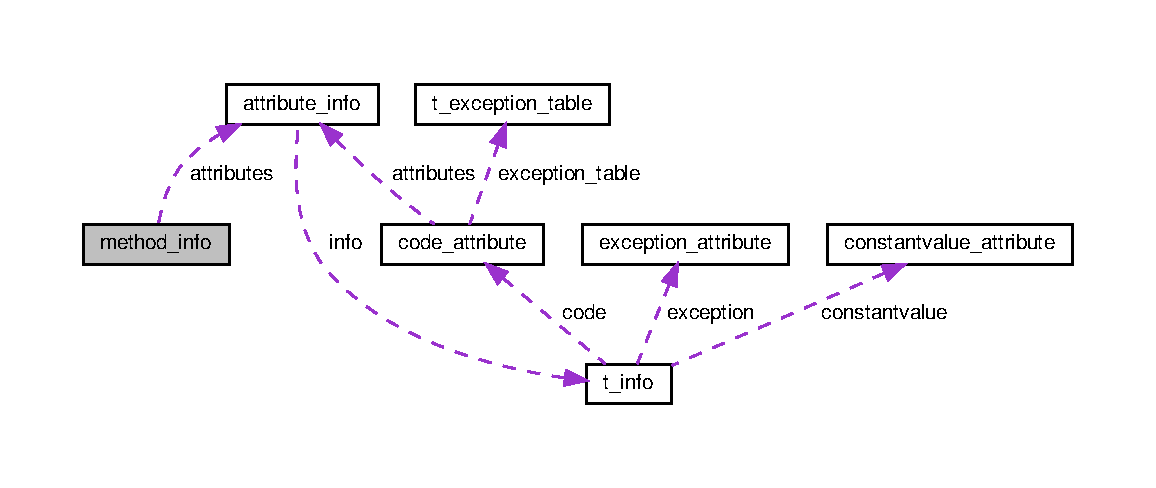
\includegraphics[width=350pt]{structmethod__info__coll__graph}
\end{center}
\end{figure}
\subsection*{Campos de Dados}
\begin{DoxyCompactItemize}
\item 
\mbox{\Hypertarget{structmethod__info_a8fc68aba419f2617deda879c467f5410}\label{structmethod__info_a8fc68aba419f2617deda879c467f5410}} 
uint16\+\_\+t {\bfseries access\+\_\+flags}
\item 
\mbox{\Hypertarget{structmethod__info_af0ba3d6d566432e74eed5c37cd998c14}\label{structmethod__info_af0ba3d6d566432e74eed5c37cd998c14}} 
uint16\+\_\+t {\bfseries name\+\_\+index}
\item 
\mbox{\Hypertarget{structmethod__info_abccd6a5202d4c0ee1be6b89692d0352a}\label{structmethod__info_abccd6a5202d4c0ee1be6b89692d0352a}} 
uint16\+\_\+t {\bfseries descriptor\+\_\+index}
\item 
\mbox{\Hypertarget{structmethod__info_a9e711e4dfb8181f7dce16c6f640ba734}\label{structmethod__info_a9e711e4dfb8181f7dce16c6f640ba734}} 
uint16\+\_\+t {\bfseries attributes\+\_\+count}
\item 
\mbox{\Hypertarget{structmethod__info_a8ce4caaa03680c91f548558a38647ad8}\label{structmethod__info_a8ce4caaa03680c91f548558a38647ad8}} 
\hyperlink{structattribute__info}{attribute\+\_\+info} $\ast$ {\bfseries attributes}
\end{DoxyCompactItemize}


A documentação para esta estrutura foi gerada a partir do seguinte ficheiro\+:\begin{DoxyCompactItemize}
\item 
include/\hyperlink{methods_8h}{methods.\+h}\end{DoxyCompactItemize}

\hypertarget{classMethodArea}{}\section{Referência à classe Method\+Area}
\label{classMethodArea}\index{Method\+Area@{Method\+Area}}


Classe responsável por todas as operações que gerenciam os métodos.  




{\ttfamily \#include $<$method\+Area.\+h$>$}

\subsection*{Membros públicos estáticos}
\begin{DoxyCompactItemize}
\item 
static \hyperlink{classClasseEstatica}{Classe\+Estatica} $\ast$ \hyperlink{classMethodArea_a81670949394fd7400fe8c006d010385e}{get\+Class} (string)
\item 
static bool \hyperlink{classMethodArea_ab67aa1b648a2dd5d78acb925501c311e}{add\+Class} (string)
\item 
static bool \hyperlink{classMethodArea_a8f781122a775565f9d99ec5603e4f432}{add\+Class} (\hyperlink{classLeitor}{Leitor} $\ast$)
\item 
static void \hyperlink{classMethodArea_af072c9b681a57a35a713b86fa61984d2}{set\+Frame\+Stack} (\hyperlink{classFrameStack}{Frame\+Stack} $\ast$)
\end{DoxyCompactItemize}
\subsection*{Atributos Públicos Estáticos}
\begin{DoxyCompactItemize}
\item 
\mbox{\Hypertarget{classMethodArea_a5fba57684c1552a65932306870b1130c}\label{classMethodArea_a5fba57684c1552a65932306870b1130c}} 
static string {\bfseries path} = \char`\"{}\char`\"{}
\end{DoxyCompactItemize}


\subsection{Descrição detalhada}
Classe responsável por todas as operações que gerenciam os métodos. 

\subsection{Documentação dos métodos}
\mbox{\Hypertarget{classMethodArea_ab67aa1b648a2dd5d78acb925501c311e}\label{classMethodArea_ab67aa1b648a2dd5d78acb925501c311e}} 
\index{Method\+Area@{Method\+Area}!add\+Class@{add\+Class}}
\index{add\+Class@{add\+Class}!Method\+Area@{Method\+Area}}
\subsubsection{\texorpdfstring{add\+Class()}{addClass()}\hspace{0.1cm}{\footnotesize\ttfamily [1/2]}}
{\footnotesize\ttfamily bool Method\+Area\+::add\+Class (\begin{DoxyParamCaption}\item[{string}]{s }\end{DoxyParamCaption})\hspace{0.3cm}{\ttfamily [static]}}

Carrega a classe na memória


\begin{DoxyParams}{Parâmetros}
{\em s} & Nome da classe \\
\hline
\end{DoxyParams}
\mbox{\Hypertarget{classMethodArea_a8f781122a775565f9d99ec5603e4f432}\label{classMethodArea_a8f781122a775565f9d99ec5603e4f432}} 
\index{Method\+Area@{Method\+Area}!add\+Class@{add\+Class}}
\index{add\+Class@{add\+Class}!Method\+Area@{Method\+Area}}
\subsubsection{\texorpdfstring{add\+Class()}{addClass()}\hspace{0.1cm}{\footnotesize\ttfamily [2/2]}}
{\footnotesize\ttfamily bool Method\+Area\+::add\+Class (\begin{DoxyParamCaption}\item[{\hyperlink{classLeitor}{Leitor} $\ast$}]{l }\end{DoxyParamCaption})\hspace{0.3cm}{\ttfamily [static]}}

Carrega classe na memória


\begin{DoxyParams}{Parâmetros}
{\em l} & informação do arquivo .class na memória \\
\hline
\end{DoxyParams}
\mbox{\Hypertarget{classMethodArea_a81670949394fd7400fe8c006d010385e}\label{classMethodArea_a81670949394fd7400fe8c006d010385e}} 
\index{Method\+Area@{Method\+Area}!get\+Class@{get\+Class}}
\index{get\+Class@{get\+Class}!Method\+Area@{Method\+Area}}
\subsubsection{\texorpdfstring{get\+Class()}{getClass()}}
{\footnotesize\ttfamily \hyperlink{classClasseEstatica}{Classe\+Estatica} $\ast$ Method\+Area\+::get\+Class (\begin{DoxyParamCaption}\item[{string}]{s }\end{DoxyParamCaption})\hspace{0.3cm}{\ttfamily [static]}}

Retorna referência para classe estática


\begin{DoxyParams}{Parâmetros}
{\em s} & Nome da classe \\
\hline
\end{DoxyParams}
\mbox{\Hypertarget{classMethodArea_af072c9b681a57a35a713b86fa61984d2}\label{classMethodArea_af072c9b681a57a35a713b86fa61984d2}} 
\index{Method\+Area@{Method\+Area}!set\+Frame\+Stack@{set\+Frame\+Stack}}
\index{set\+Frame\+Stack@{set\+Frame\+Stack}!Method\+Area@{Method\+Area}}
\subsubsection{\texorpdfstring{set\+Frame\+Stack()}{setFrameStack()}}
{\footnotesize\ttfamily void Method\+Area\+::set\+Frame\+Stack (\begin{DoxyParamCaption}\item[{\hyperlink{classFrameStack}{Frame\+Stack} $\ast$}]{new\+FS }\end{DoxyParamCaption})\hspace{0.3cm}{\ttfamily [static]}}

Atualiza a referência da pilha de frames para o próximo frame


\begin{DoxyParams}{Parâmetros}
{\em new\+FS} & próximo frame \\
\hline
\end{DoxyParams}


A documentação para esta classe foi gerada a partir dos seguintes ficheiros\+:\begin{DoxyCompactItemize}
\item 
include/\hyperlink{methodArea_8h}{method\+Area.\+h}\item 
src/method\+Area.\+cpp\end{DoxyCompactItemize}

\hypertarget{structn__array}{}\section{Referência à estrutura n\+\_\+array}
\label{structn__array}\index{n\+\_\+array@{n\+\_\+array}}
\subsection*{Campos de Dados}
\begin{DoxyCompactItemize}
\item 
\mbox{\Hypertarget{structn__array_a87c94199251d7ab8daf6870960bf61c2}\label{structn__array_a87c94199251d7ab8daf6870960bf61c2}} 
int $\ast$ {\bfseries dims}
\item 
\mbox{\Hypertarget{structn__array_aeb0cc650d775c11f48315cef8e3834de}\label{structn__array_aeb0cc650d775c11f48315cef8e3834de}} 
int $\ast$ {\bfseries array}
\end{DoxyCompactItemize}


A documentação para esta estrutura foi gerada a partir do seguinte ficheiro\+:\begin{DoxyCompactItemize}
\item 
include/\hyperlink{baseTypes_8h}{base\+Types.\+h}\end{DoxyCompactItemize}

\hypertarget{classOperacoes}{}\section{Referência à classe Operacoes}
\label{classOperacoes}\index{Operacoes@{Operacoes}}
\subsection*{Membros públicos}
\begin{DoxyCompactItemize}
\item 
\mbox{\Hypertarget{classOperacoes_a2122b7e6890e56a386118b62b32a7523}\label{classOperacoes_a2122b7e6890e56a386118b62b32a7523}} 
{\bfseries Operacoes} (struct \hyperlink{structframe__s}{frame\+\_\+s} $\ast$)
\end{DoxyCompactItemize}
\subsection*{Membros públicos estáticos}
\begin{DoxyCompactItemize}
\item 
\mbox{\Hypertarget{classOperacoes_a787f291554d319e73daa2e91d77823bd}\label{classOperacoes_a787f291554d319e73daa2e91d77823bd}} 
static void {\bfseries set\+Frame} (struct \hyperlink{structframe__s}{frame\+\_\+s} $\ast$)
\item 
\mbox{\Hypertarget{classOperacoes_ac50ddb76ffb9bcd17ac19e449ac52e39}\label{classOperacoes_ac50ddb76ffb9bcd17ac19e449ac52e39}} 
static void {\bfseries set\+Threads} (stack$<$ struct \hyperlink{structframe__s}{frame\+\_\+s} $\ast$$>$ $\ast$)
\item 
\mbox{\Hypertarget{classOperacoes_a458ce9c1aec4fd809eecee9b005fcbf5}\label{classOperacoes_a458ce9c1aec4fd809eecee9b005fcbf5}} 
static void {\bfseries set\+Frame\+Stack} (\hyperlink{classFrameStack}{Frame\+Stack} $\ast$)
\item 
\mbox{\Hypertarget{classOperacoes_ac25eec2246429c071161b918ec447b18}\label{classOperacoes_ac25eec2246429c071161b918ec447b18}} 
static void {\bfseries run} (int)
\end{DoxyCompactItemize}


A documentação para esta classe foi gerada a partir dos seguintes ficheiros\+:\begin{DoxyCompactItemize}
\item 
include/\hyperlink{operacoes_8h}{operacoes.\+h}\item 
src/\hyperlink{operacoes_8cpp}{operacoes.\+cpp}\end{DoxyCompactItemize}

\hypertarget{classPilhaOperandos}{}\section{Referência à classe Pilha\+Operandos}
\label{classPilhaOperandos}\index{Pilha\+Operandos@{Pilha\+Operandos}}


Classe da pilha de operandos.  




{\ttfamily \#include $<$pilha\+Operandos.\+h$>$}

\subsection*{Membros públicos}
\begin{DoxyCompactItemize}
\item 
\hyperlink{classPilhaOperandos_ab17dc4822af4e7e7c0962152d93547c6}{Pilha\+Operandos} (int)
\begin{DoxyCompactList}\small\item\em Construtor. \end{DoxyCompactList}\item 
uint8\+\_\+t \hyperlink{classPilhaOperandos_ab44ede250e434c1bb17f21d787977f20}{top\+\_\+type} ()
\begin{DoxyCompactList}\small\item\em Recupera o tipo do topo da pilha de operandos. \end{DoxyCompactList}\item 
\hyperlink{unionelement__u}{element} \hyperlink{classPilhaOperandos_a2fadf264a2a34fc52f89ef7e1e62f19b}{top\+\_\+value} ()
\begin{DoxyCompactList}\small\item\em Recupera o valor do topo da pilha de operandos. \end{DoxyCompactList}\item 
\hyperlink{unionelement__u}{element} \hyperlink{classPilhaOperandos_a17a3e3f5e3caad834db7653b2c17ef24}{pop} ()
\begin{DoxyCompactList}\small\item\em Desempilha o topo da pilha de operandos e retorna em um elemento de valor. \end{DoxyCompactList}\item 
\hyperlink{structtypedElement__s}{typed\+Element} \hyperlink{classPilhaOperandos_a9dd3f7998df13b3bef6f13a1edecf3a4}{pop\+Typed} ()
\item 
std\+::string \hyperlink{classPilhaOperandos_a26d2bb2bcaf156c09ed688958a6f00e2}{get\+String} ()
\begin{DoxyCompactList}\small\item\em Retorna o topo da pilha de operandos formatado em uma string. \end{DoxyCompactList}\item 
void \hyperlink{classPilhaOperandos_aebcb6ec63863f3f273f2ded4331de26a}{push} (int)
\begin{DoxyCompactList}\small\item\em Empilha um valor de tipo inteiro. \end{DoxyCompactList}\item 
void \hyperlink{classPilhaOperandos_a6f8e84e9eeaac29d5607d0e87d7a566a}{push} (int64\+\_\+t)
\item 
void \hyperlink{classPilhaOperandos_ab696a021a389db273c043bedf1e5f4d6}{push} (float)
\begin{DoxyCompactList}\small\item\em Empilha um valor de tipo float. \end{DoxyCompactList}\item 
void \hyperlink{classPilhaOperandos_a4b55bb7ee498ded849f19702e602fe85}{push} (double)
\begin{DoxyCompactList}\small\item\em Empilha um valor de tipo double. \end{DoxyCompactList}\item 
void \hyperlink{classPilhaOperandos_a76e6e4b9d47f9e549e4a9d76aef6d89d}{push} (bool)
\begin{DoxyCompactList}\small\item\em Empilha um valor de tipo double. \end{DoxyCompactList}\item 
void \hyperlink{classPilhaOperandos_aef0bd19eae8107546d419aba6d7c2d47}{push} (int $\ast$)
\begin{DoxyCompactList}\small\item\em Empilha um valor de tipo referencia. \end{DoxyCompactList}\item 
void \hyperlink{classPilhaOperandos_a2a8591e6f42cee7186ee70e0fa998208}{push} (\hyperlink{structtypedElement__s}{typed\+Element})
\begin{DoxyCompactList}\small\item\em Empilha um elemento tipado, chamando a fun��o adequada ao tipo. \end{DoxyCompactList}\item 
void \hyperlink{classPilhaOperandos_a7879a301351feee2cd4bbd7639e44822}{push} (\hyperlink{unionelement__u}{element}, uint8\+\_\+t)
\begin{DoxyCompactList}\small\item\em Verifica o tipo do elemento que deve ser empilhado e chama a fun��o adequada. \end{DoxyCompactList}\item 
int \hyperlink{classPilhaOperandos_a3db3fb4dd085cd2f7454a92e93b7ad3c}{size} ()
\begin{DoxyCompactList}\small\item\em Verifica o tamanho da pilha de operandos. \end{DoxyCompactList}\item 
int \hyperlink{classPilhaOperandos_a6de0f5994b22c1c0b3d903e233bbf6fe}{get\+Max\+Size} ()
\begin{DoxyCompactList}\small\item\em Retorna o tamanho m�ximo da pilha de operandos. \end{DoxyCompactList}\item 
bool \hyperlink{classPilhaOperandos_a4099bf8202558794b12086c410da3e16}{empty} ()
\begin{DoxyCompactList}\small\item\em Retorna se a pilha est� vazia (1) ou n�o (0) \end{DoxyCompactList}\item 
void \hyperlink{classPilhaOperandos_ab0f7d8632714842751483b7463e34efb}{print\+A\+LL} ()
\end{DoxyCompactItemize}
\subsection*{Campos de Dados}
\begin{DoxyCompactItemize}
\item 
\mbox{\Hypertarget{classPilhaOperandos_a010c46a6b2a726067e823fa5488414af}\label{classPilhaOperandos_a010c46a6b2a726067e823fa5488414af}} 
const int {\bfseries max}
\end{DoxyCompactItemize}


\subsection{Descrição detalhada}
Classe da pilha de operandos. 

Respons�vel por armazenar e manipular a pilha de operandos 

\subsection{Documentação dos Construtores \& Destrutor}
\mbox{\Hypertarget{classPilhaOperandos_ab17dc4822af4e7e7c0962152d93547c6}\label{classPilhaOperandos_ab17dc4822af4e7e7c0962152d93547c6}} 
\index{Pilha\+Operandos@{Pilha\+Operandos}!Pilha\+Operandos@{Pilha\+Operandos}}
\index{Pilha\+Operandos@{Pilha\+Operandos}!Pilha\+Operandos@{Pilha\+Operandos}}
\subsubsection{\texorpdfstring{Pilha\+Operandos()}{PilhaOperandos()}}
{\footnotesize\ttfamily Pilha\+Operandos\+::\+Pilha\+Operandos (\begin{DoxyParamCaption}\item[{int}]{max\+Size }\end{DoxyParamCaption})}



Construtor. 

Construtor


\begin{DoxyParams}{Parâmetros}
{\em max\+Size} & Indica tamanho m�ximo da pilha de operandos \\
\hline
\end{DoxyParams}


\subsection{Documentação dos métodos}
\mbox{\Hypertarget{classPilhaOperandos_a4099bf8202558794b12086c410da3e16}\label{classPilhaOperandos_a4099bf8202558794b12086c410da3e16}} 
\index{Pilha\+Operandos@{Pilha\+Operandos}!empty@{empty}}
\index{empty@{empty}!Pilha\+Operandos@{Pilha\+Operandos}}
\subsubsection{\texorpdfstring{empty()}{empty()}}
{\footnotesize\ttfamily bool Pilha\+Operandos\+::empty (\begin{DoxyParamCaption}{ }\end{DoxyParamCaption})}



Retorna se a pilha est� vazia (1) ou n�o (0) 

returna 1 se a pilha de valores estiver vazia, 0 caso contr�rio \mbox{\Hypertarget{classPilhaOperandos_a6de0f5994b22c1c0b3d903e233bbf6fe}\label{classPilhaOperandos_a6de0f5994b22c1c0b3d903e233bbf6fe}} 
\index{Pilha\+Operandos@{Pilha\+Operandos}!get\+Max\+Size@{get\+Max\+Size}}
\index{get\+Max\+Size@{get\+Max\+Size}!Pilha\+Operandos@{Pilha\+Operandos}}
\subsubsection{\texorpdfstring{get\+Max\+Size()}{getMaxSize()}}
{\footnotesize\ttfamily int Pilha\+Operandos\+::get\+Max\+Size (\begin{DoxyParamCaption}{ }\end{DoxyParamCaption})}



Retorna o tamanho m�ximo da pilha de operandos. 

Retorna valor m�ximo da pilha de operandos \mbox{\Hypertarget{classPilhaOperandos_a26d2bb2bcaf156c09ed688958a6f00e2}\label{classPilhaOperandos_a26d2bb2bcaf156c09ed688958a6f00e2}} 
\index{Pilha\+Operandos@{Pilha\+Operandos}!get\+String@{get\+String}}
\index{get\+String@{get\+String}!Pilha\+Operandos@{Pilha\+Operandos}}
\subsubsection{\texorpdfstring{get\+String()}{getString()}}
{\footnotesize\ttfamily std\+::string Pilha\+Operandos\+::get\+String (\begin{DoxyParamCaption}{ }\end{DoxyParamCaption})}



Retorna o topo da pilha de operandos formatado em uma string. 

Auxiliar do print\+All, imprime a string correspondente ao tipo do elemento \mbox{\Hypertarget{classPilhaOperandos_a17a3e3f5e3caad834db7653b2c17ef24}\label{classPilhaOperandos_a17a3e3f5e3caad834db7653b2c17ef24}} 
\index{Pilha\+Operandos@{Pilha\+Operandos}!pop@{pop}}
\index{pop@{pop}!Pilha\+Operandos@{Pilha\+Operandos}}
\subsubsection{\texorpdfstring{pop()}{pop()}}
{\footnotesize\ttfamily \hyperlink{unionelement__u}{element} Pilha\+Operandos\+::pop (\begin{DoxyParamCaption}{ }\end{DoxyParamCaption})}



Desempilha o topo da pilha de operandos e retorna em um elemento de valor. 

Desempilha o topo da pilha de operandos e retorna em um elemento tipado.

Retorna e remove topo da pilha de valores e da pop na pilha de tipos \mbox{\Hypertarget{classPilhaOperandos_a9dd3f7998df13b3bef6f13a1edecf3a4}\label{classPilhaOperandos_a9dd3f7998df13b3bef6f13a1edecf3a4}} 
\index{Pilha\+Operandos@{Pilha\+Operandos}!pop\+Typed@{pop\+Typed}}
\index{pop\+Typed@{pop\+Typed}!Pilha\+Operandos@{Pilha\+Operandos}}
\subsubsection{\texorpdfstring{pop\+Typed()}{popTyped()}}
{\footnotesize\ttfamily \hyperlink{structtypedElement__s}{typed\+Element} Pilha\+Operandos\+::pop\+Typed (\begin{DoxyParamCaption}{ }\end{DoxyParamCaption})}

Retorna estrutura com valor e tipo associados e da pop na pilha de valores e na de tipos \mbox{\Hypertarget{classPilhaOperandos_ab0f7d8632714842751483b7463e34efb}\label{classPilhaOperandos_ab0f7d8632714842751483b7463e34efb}} 
\index{Pilha\+Operandos@{Pilha\+Operandos}!print\+A\+LL@{print\+A\+LL}}
\index{print\+A\+LL@{print\+A\+LL}!Pilha\+Operandos@{Pilha\+Operandos}}
\subsubsection{\texorpdfstring{print\+A\+L\+L()}{printALL()}}
{\footnotesize\ttfamily void Pilha\+Operandos\+::print\+A\+LL (\begin{DoxyParamCaption}{ }\end{DoxyParamCaption})}

Percorre e imprime toda a pilha de operandos \mbox{\Hypertarget{classPilhaOperandos_aebcb6ec63863f3f273f2ded4331de26a}\label{classPilhaOperandos_aebcb6ec63863f3f273f2ded4331de26a}} 
\index{Pilha\+Operandos@{Pilha\+Operandos}!push@{push}}
\index{push@{push}!Pilha\+Operandos@{Pilha\+Operandos}}
\subsubsection{\texorpdfstring{push()}{push()}\hspace{0.1cm}{\footnotesize\ttfamily [1/8]}}
{\footnotesize\ttfamily void Pilha\+Operandos\+::push (\begin{DoxyParamCaption}\item[{int}]{x }\end{DoxyParamCaption})}



Empilha um valor de tipo inteiro. 

Empilha um int na pilha de valores e seu tipo na pilha de tipos


\begin{DoxyParams}{Parâmetros}
{\em x} & Valor a ser empilhado \\
\hline
\end{DoxyParams}
\mbox{\Hypertarget{classPilhaOperandos_a6f8e84e9eeaac29d5607d0e87d7a566a}\label{classPilhaOperandos_a6f8e84e9eeaac29d5607d0e87d7a566a}} 
\index{Pilha\+Operandos@{Pilha\+Operandos}!push@{push}}
\index{push@{push}!Pilha\+Operandos@{Pilha\+Operandos}}
\subsubsection{\texorpdfstring{push()}{push()}\hspace{0.1cm}{\footnotesize\ttfamily [2/8]}}
{\footnotesize\ttfamily void Pilha\+Operandos\+::push (\begin{DoxyParamCaption}\item[{int64\+\_\+t}]{\+\_\+x }\end{DoxyParamCaption})}

Empilha um long na pilha de valores e seu tipo na pilha de tipos \mbox{\Hypertarget{classPilhaOperandos_ab696a021a389db273c043bedf1e5f4d6}\label{classPilhaOperandos_ab696a021a389db273c043bedf1e5f4d6}} 
\index{Pilha\+Operandos@{Pilha\+Operandos}!push@{push}}
\index{push@{push}!Pilha\+Operandos@{Pilha\+Operandos}}
\subsubsection{\texorpdfstring{push()}{push()}\hspace{0.1cm}{\footnotesize\ttfamily [3/8]}}
{\footnotesize\ttfamily void Pilha\+Operandos\+::push (\begin{DoxyParamCaption}\item[{float}]{x }\end{DoxyParamCaption})}



Empilha um valor de tipo float. 

Empilha um float na pilha de valores e seu tipo na pilha de tipos


\begin{DoxyParams}{Parâmetros}
{\em x} & Valor a ser empilhado \\
\hline
\end{DoxyParams}
\mbox{\Hypertarget{classPilhaOperandos_a4b55bb7ee498ded849f19702e602fe85}\label{classPilhaOperandos_a4b55bb7ee498ded849f19702e602fe85}} 
\index{Pilha\+Operandos@{Pilha\+Operandos}!push@{push}}
\index{push@{push}!Pilha\+Operandos@{Pilha\+Operandos}}
\subsubsection{\texorpdfstring{push()}{push()}\hspace{0.1cm}{\footnotesize\ttfamily [4/8]}}
{\footnotesize\ttfamily void Pilha\+Operandos\+::push (\begin{DoxyParamCaption}\item[{double}]{x }\end{DoxyParamCaption})}



Empilha um valor de tipo double. 

Empilha um double na pilha de valores e seu tipo na pilha de tipos


\begin{DoxyParams}{Parâmetros}
{\em x} & Valor a ser empilhado \\
\hline
\end{DoxyParams}
\mbox{\Hypertarget{classPilhaOperandos_a76e6e4b9d47f9e549e4a9d76aef6d89d}\label{classPilhaOperandos_a76e6e4b9d47f9e549e4a9d76aef6d89d}} 
\index{Pilha\+Operandos@{Pilha\+Operandos}!push@{push}}
\index{push@{push}!Pilha\+Operandos@{Pilha\+Operandos}}
\subsubsection{\texorpdfstring{push()}{push()}\hspace{0.1cm}{\footnotesize\ttfamily [5/8]}}
{\footnotesize\ttfamily void Pilha\+Operandos\+::push (\begin{DoxyParamCaption}\item[{bool}]{x }\end{DoxyParamCaption})}



Empilha um valor de tipo double. 

Empilha um bool na pilha de valores e seu tipo na pilha de tipos


\begin{DoxyParams}{Parâmetros}
{\em x} & Valor a ser empilhado \\
\hline
\end{DoxyParams}
\mbox{\Hypertarget{classPilhaOperandos_aef0bd19eae8107546d419aba6d7c2d47}\label{classPilhaOperandos_aef0bd19eae8107546d419aba6d7c2d47}} 
\index{Pilha\+Operandos@{Pilha\+Operandos}!push@{push}}
\index{push@{push}!Pilha\+Operandos@{Pilha\+Operandos}}
\subsubsection{\texorpdfstring{push()}{push()}\hspace{0.1cm}{\footnotesize\ttfamily [6/8]}}
{\footnotesize\ttfamily void Pilha\+Operandos\+::push (\begin{DoxyParamCaption}\item[{int $\ast$}]{x }\end{DoxyParamCaption})}



Empilha um valor de tipo referencia. 

Empilha uma referencia na pilha de valores e seu tipo na pilha de tipos


\begin{DoxyParams}{Parâmetros}
{\em x} & Referencia a ser empilhada \\
\hline
\end{DoxyParams}
\mbox{\Hypertarget{classPilhaOperandos_a2a8591e6f42cee7186ee70e0fa998208}\label{classPilhaOperandos_a2a8591e6f42cee7186ee70e0fa998208}} 
\index{Pilha\+Operandos@{Pilha\+Operandos}!push@{push}}
\index{push@{push}!Pilha\+Operandos@{Pilha\+Operandos}}
\subsubsection{\texorpdfstring{push()}{push()}\hspace{0.1cm}{\footnotesize\ttfamily [7/8]}}
{\footnotesize\ttfamily void Pilha\+Operandos\+::push (\begin{DoxyParamCaption}\item[{\hyperlink{structtypedElement__s}{typed\+Element}}]{te }\end{DoxyParamCaption})}



Empilha um elemento tipado, chamando a fun��o adequada ao tipo. 

Empilha valor e tipo de estrutura com valor e tipo associados


\begin{DoxyParams}{Parâmetros}
{\em x} & Elemento tipado a ser empilhado \\
\hline
\end{DoxyParams}
\mbox{\Hypertarget{classPilhaOperandos_a7879a301351feee2cd4bbd7639e44822}\label{classPilhaOperandos_a7879a301351feee2cd4bbd7639e44822}} 
\index{Pilha\+Operandos@{Pilha\+Operandos}!push@{push}}
\index{push@{push}!Pilha\+Operandos@{Pilha\+Operandos}}
\subsubsection{\texorpdfstring{push()}{push()}\hspace{0.1cm}{\footnotesize\ttfamily [8/8]}}
{\footnotesize\ttfamily void Pilha\+Operandos\+::push (\begin{DoxyParamCaption}\item[{\hyperlink{unionelement__u}{element}}]{x,  }\item[{uint8\+\_\+t}]{tipo }\end{DoxyParamCaption})}



Verifica o tipo do elemento que deve ser empilhado e chama a fun��o adequada. 

Chama a fun��o para empilhar de acordo com o tipo do elemento recebido


\begin{DoxyParams}{Parâmetros}
{\em x} & Elemento a ser empilhado \\
\hline
{\em tipo} & Tipo do elemento a ser empilhado \\
\hline
\end{DoxyParams}
\mbox{\Hypertarget{classPilhaOperandos_a3db3fb4dd085cd2f7454a92e93b7ad3c}\label{classPilhaOperandos_a3db3fb4dd085cd2f7454a92e93b7ad3c}} 
\index{Pilha\+Operandos@{Pilha\+Operandos}!size@{size}}
\index{size@{size}!Pilha\+Operandos@{Pilha\+Operandos}}
\subsubsection{\texorpdfstring{size()}{size()}}
{\footnotesize\ttfamily int Pilha\+Operandos\+::size (\begin{DoxyParamCaption}{ }\end{DoxyParamCaption})}



Verifica o tamanho da pilha de operandos. 

Retorna o tamanho da pilha de valores \mbox{\Hypertarget{classPilhaOperandos_ab44ede250e434c1bb17f21d787977f20}\label{classPilhaOperandos_ab44ede250e434c1bb17f21d787977f20}} 
\index{Pilha\+Operandos@{Pilha\+Operandos}!top\+\_\+type@{top\+\_\+type}}
\index{top\+\_\+type@{top\+\_\+type}!Pilha\+Operandos@{Pilha\+Operandos}}
\subsubsection{\texorpdfstring{top\+\_\+type()}{top\_type()}}
{\footnotesize\ttfamily uint8\+\_\+t Pilha\+Operandos\+::top\+\_\+type (\begin{DoxyParamCaption}{ }\end{DoxyParamCaption})}



Recupera o tipo do topo da pilha de operandos. 

Retorna topo da pilha de tipos \mbox{\Hypertarget{classPilhaOperandos_a2fadf264a2a34fc52f89ef7e1e62f19b}\label{classPilhaOperandos_a2fadf264a2a34fc52f89ef7e1e62f19b}} 
\index{Pilha\+Operandos@{Pilha\+Operandos}!top\+\_\+value@{top\+\_\+value}}
\index{top\+\_\+value@{top\+\_\+value}!Pilha\+Operandos@{Pilha\+Operandos}}
\subsubsection{\texorpdfstring{top\+\_\+value()}{top\_value()}}
{\footnotesize\ttfamily \hyperlink{unionelement__u}{element} Pilha\+Operandos\+::top\+\_\+value (\begin{DoxyParamCaption}{ }\end{DoxyParamCaption})}



Recupera o valor do topo da pilha de operandos. 

Retorna topo da pilha de valores 

A documentação para esta classe foi gerada a partir dos seguintes ficheiros\+:\begin{DoxyCompactItemize}
\item 
include/\hyperlink{pilhaOperandos_8h}{pilha\+Operandos.\+h}\item 
src/\hyperlink{pilhaOperandos_8cpp}{pilha\+Operandos.\+cpp}\end{DoxyCompactItemize}

\hypertarget{structt__exception__table}{}\section{Referência à estrutura t\+\_\+exception\+\_\+table}
\label{structt__exception__table}\index{t\+\_\+exception\+\_\+table@{t\+\_\+exception\+\_\+table}}


Struct para salvar exceções identificadas. Será utilizada como componente da struct \char`\"{}code\+\_\+attribute\char`\"{}.  




{\ttfamily \#include $<$attributes.\+h$>$}

\subsection*{Campos de Dados}
\begin{DoxyCompactItemize}
\item 
\mbox{\Hypertarget{structt__exception__table_a1e301f7924e5e2ebe75dbf5a4bb2b090}\label{structt__exception__table_a1e301f7924e5e2ebe75dbf5a4bb2b090}} 
unsigned short {\bfseries start\+\_\+pc}
\item 
\mbox{\Hypertarget{structt__exception__table_a0e650c1f5254b1163fb64c19524e45cf}\label{structt__exception__table_a0e650c1f5254b1163fb64c19524e45cf}} 
unsigned short {\bfseries end\+\_\+pc}
\item 
\mbox{\Hypertarget{structt__exception__table_adeddab7249cce7351d5f8387ccae0963}\label{structt__exception__table_adeddab7249cce7351d5f8387ccae0963}} 
unsigned short {\bfseries handler\+\_\+pc}
\item 
\mbox{\Hypertarget{structt__exception__table_a948e8861147a4c9ce9df40ca1f5cf680}\label{structt__exception__table_a948e8861147a4c9ce9df40ca1f5cf680}} 
unsigned short {\bfseries catch\+\_\+type}
\end{DoxyCompactItemize}


\subsection{Descrição detalhada}
Struct para salvar exceções identificadas. Será utilizada como componente da struct \char`\"{}code\+\_\+attribute\char`\"{}. 

A documentação para esta estrutura foi gerada a partir do seguinte ficheiro\+:\begin{DoxyCompactItemize}
\item 
include/\hyperlink{attributes_8h}{attributes.\+h}\end{DoxyCompactItemize}

\hypertarget{uniont__info}{}\section{Referência à união t\+\_\+info}
\label{uniont__info}\index{t\+\_\+info@{t\+\_\+info}}


Estrutura de dados que agrega informações sobre cada atributo lido.  




{\ttfamily \#include $<$attributes.\+h$>$}



Diagrama de colaboração para t\+\_\+info\+:
\nopagebreak
\begin{figure}[H]
\begin{center}
\leavevmode
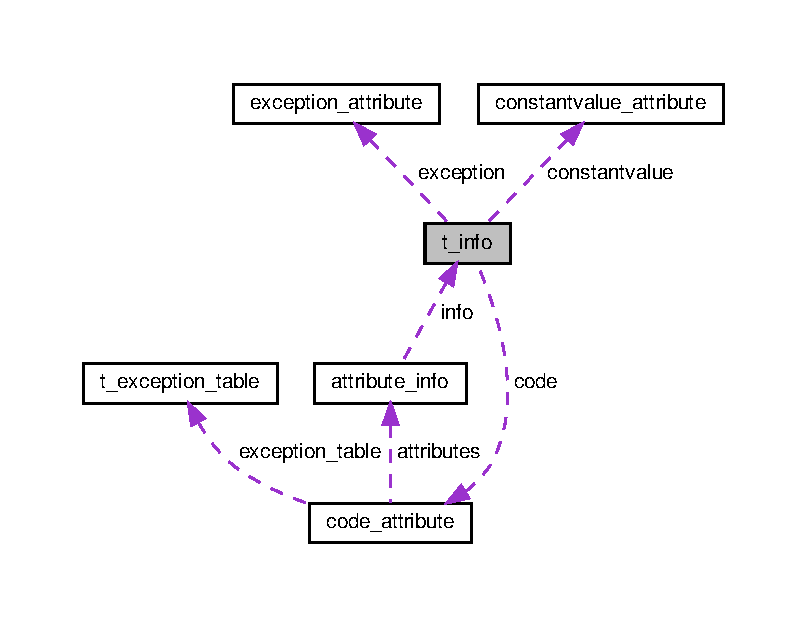
\includegraphics[width=350pt]{uniont__info__coll__graph}
\end{center}
\end{figure}
\subsection*{Campos de Dados}
\begin{DoxyCompactItemize}
\item 
\mbox{\Hypertarget{uniont__info_ab4a27f0438794e6a65bbdd9776fe657a}\label{uniont__info_ab4a27f0438794e6a65bbdd9776fe657a}} 
\hyperlink{structconstantvalue__attribute}{constantvalue\+\_\+attribute} {\bfseries constantvalue}
\item 
\mbox{\Hypertarget{uniont__info_a71f98a8da1881861b03ab649c3c7a788}\label{uniont__info_a71f98a8da1881861b03ab649c3c7a788}} 
\hyperlink{structcode__attribute}{code\+\_\+attribute} {\bfseries code}
\item 
\mbox{\Hypertarget{uniont__info_ad8bba19df869f74ce8cb48ae37c3fff4}\label{uniont__info_ad8bba19df869f74ce8cb48ae37c3fff4}} 
\hyperlink{structexception__attribute}{exception\+\_\+attribute} {\bfseries exception}
\end{DoxyCompactItemize}


\subsection{Descrição detalhada}
Estrutura de dados que agrega informações sobre cada atributo lido. 

A documentação para esta união foi gerada a partir do seguinte ficheiro\+:\begin{DoxyCompactItemize}
\item 
include/\hyperlink{attributes_8h}{attributes.\+h}\end{DoxyCompactItemize}

\hypertarget{structtypedElement__s}{}\section{Referência à estrutura typed\+Element\+\_\+s}
\label{structtypedElement__s}\index{typed\+Element\+\_\+s@{typed\+Element\+\_\+s}}


Agregador de tipos e informações. Struct responsável por juntar tipos e informações de elementos.  




{\ttfamily \#include $<$base\+Types.\+h$>$}



Diagrama de colaboração para typed\+Element\+\_\+s\+:\nopagebreak
\begin{figure}[H]
\begin{center}
\leavevmode
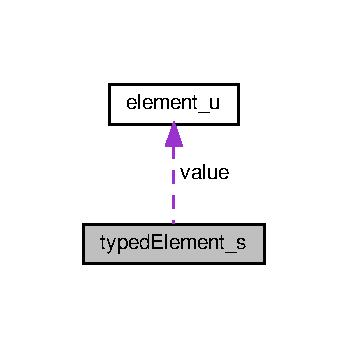
\includegraphics[width=167pt]{structtypedElement__s__coll__graph}
\end{center}
\end{figure}
\subsection*{Campos de Dados}
\begin{DoxyCompactItemize}
\item 
\mbox{\Hypertarget{structtypedElement__s_a579b7dd61dd13e2a1d37035d3758a2dc}\label{structtypedElement__s_a579b7dd61dd13e2a1d37035d3758a2dc}} 
\hyperlink{unionelement__u}{element} {\bfseries value}
\item 
\mbox{\Hypertarget{structtypedElement__s_a725ddec1b2a04b6488cdde81f3e0255e}\label{structtypedElement__s_a725ddec1b2a04b6488cdde81f3e0255e}} 
uint8\+\_\+t {\bfseries type}
\item 
\mbox{\Hypertarget{structtypedElement__s_a265d7ad822f91bfa8fd6eb292e2d20d8}\label{structtypedElement__s_a265d7ad822f91bfa8fd6eb292e2d20d8}} 
uint8\+\_\+t {\bfseries real\+Type}
\end{DoxyCompactItemize}


\subsection{Descrição detalhada}
Agregador de tipos e informações. Struct responsável por juntar tipos e informações de elementos. 

A documentação para esta estrutura foi gerada a partir do seguinte ficheiro\+:\begin{DoxyCompactItemize}
\item 
include/\hyperlink{baseTypes_8h}{base\+Types.\+h}\end{DoxyCompactItemize}

\chapter{Documentação do ficheiro}
\hypertarget{attributes_8h}{}\section{Referência ao ficheiro include/attributes.h}
\label{attributes_8h}\index{include/attributes.\+h@{include/attributes.\+h}}


Atributos a serem usados na execuçao da J\+VM.  


{\ttfamily \#include $<$iostream$>$}\newline
{\ttfamily \#include $<$stdlib.\+h$>$}\newline
{\ttfamily \#include $<$string$>$}\newline
{\ttfamily \#include \char`\"{}constant\+Pool.\+h\char`\"{}}\newline
Diagrama de dependências de inclusão para attributes.\+h\+:
\nopagebreak
\begin{figure}[H]
\begin{center}
\leavevmode
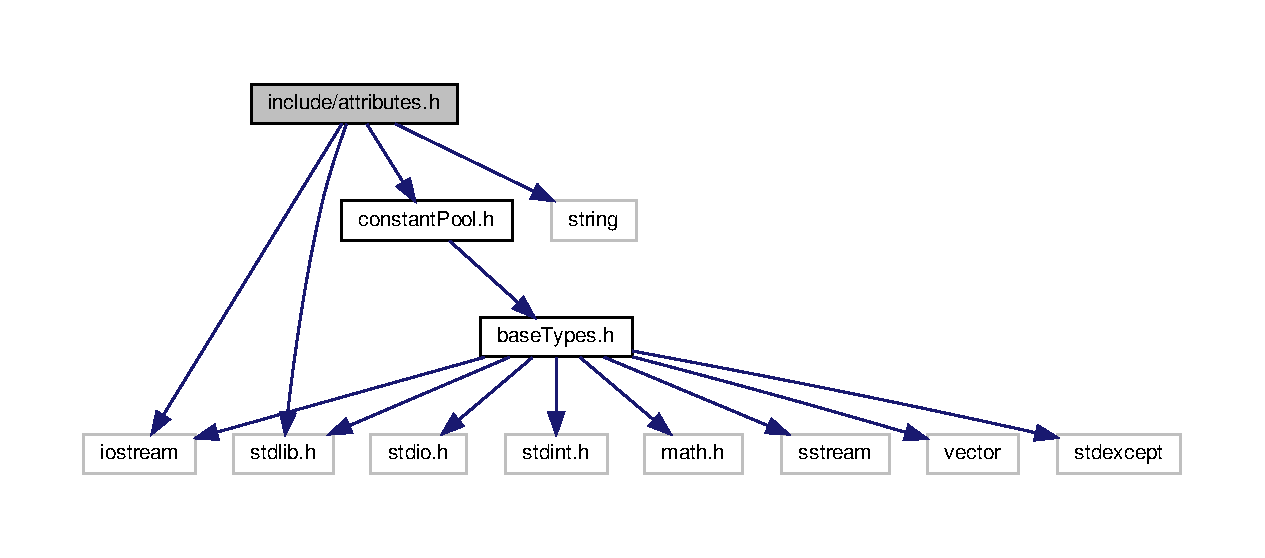
\includegraphics[width=350pt]{attributes_8h__incl}
\end{center}
\end{figure}
Este grafo mostra quais são os ficheiros que incluem directamente ou indirectamente este ficheiro\+:
\nopagebreak
\begin{figure}[H]
\begin{center}
\leavevmode
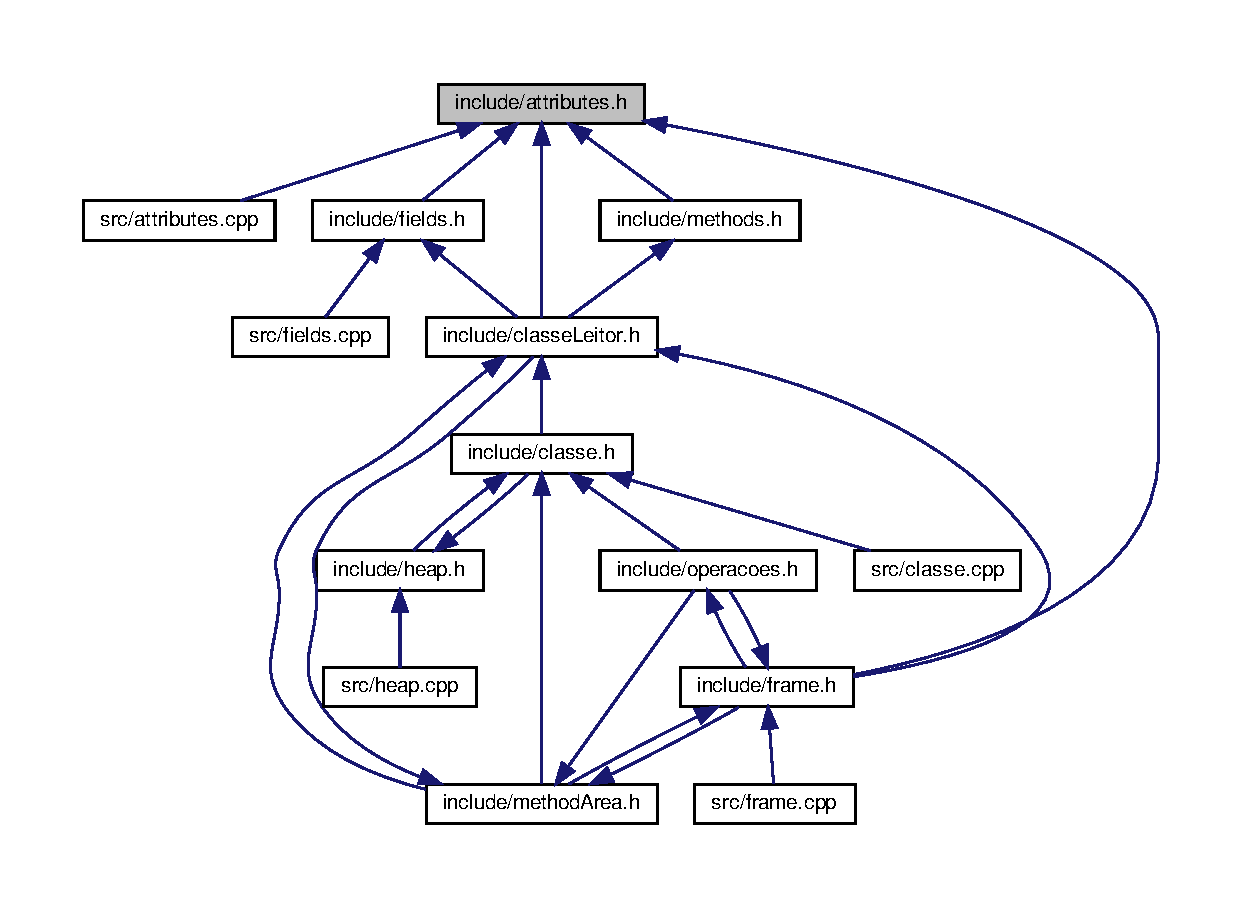
\includegraphics[width=350pt]{attributes_8h__dep__incl}
\end{center}
\end{figure}
\subsection*{Estruturas de Dados}
\begin{DoxyCompactItemize}
\item 
struct \hyperlink{structconstantvalue__attribute}{constantvalue\+\_\+attribute}
\begin{DoxyCompactList}\small\item\em Struct para carregar o index dos atributos da \char`\"{}constantpool\char`\"{}. \end{DoxyCompactList}\item 
struct \hyperlink{structt__exception__table}{t\+\_\+exception\+\_\+table}
\begin{DoxyCompactList}\small\item\em Struct para salvar exceções identificadas. Será utilizada como componente da struct \char`\"{}code\+\_\+attribute\char`\"{}. \end{DoxyCompactList}\item 
struct \hyperlink{structcode__attribute}{code\+\_\+attribute}
\begin{DoxyCompactList}\small\item\em Estrutura de dados para salvar atributos do tipo code. \end{DoxyCompactList}\item 
struct \hyperlink{structexception__attribute}{exception\+\_\+attribute}
\item 
union \hyperlink{uniont__info}{t\+\_\+info}
\begin{DoxyCompactList}\small\item\em Estrutura de dados que agrega informações sobre cada atributo lido. \end{DoxyCompactList}\item 
struct \hyperlink{structattribute__info}{attribute\+\_\+info}
\begin{DoxyCompactList}\small\item\em Estrutura de dados para salvar a posição do atributo na constantpool e seu tamanho. \end{DoxyCompactList}\end{DoxyCompactItemize}
\subsection*{Funções}
\begin{DoxyCompactItemize}
\item 
\hyperlink{structt__exception__table}{t\+\_\+exception\+\_\+table} $\ast$ \hyperlink{attributes_8h_a7074ce92141e1009d4bfcbc1eda14ddb}{read\+Exception\+Handler} (F\+I\+LE $\ast$fp)
\begin{DoxyCompactList}\small\item\em Função de leitura de exceções. \end{DoxyCompactList}\item 
\hyperlink{uniont__info}{t\+\_\+info} $\ast$ \hyperlink{attributes_8h_aaf5bf869e6d94d4dbf72884249a91431}{read\+Attribute\+Info} (F\+I\+LE $\ast$fp, \hyperlink{structcp__info}{cp\+\_\+info} $\ast$cp, unsigned short index, unsigned short length)
\begin{DoxyCompactList}\small\item\em Faz a leitura das informações de um atributo. \end{DoxyCompactList}\item 
\hyperlink{structattribute__info}{attribute\+\_\+info} \hyperlink{attributes_8h_a1f014ecafdc1b309e228f89cff54d61e}{read\+Attribute} (F\+I\+LE $\ast$fp, \hyperlink{structcp__info}{cp\+\_\+info} $\ast$cp)
\begin{DoxyCompactList}\small\item\em Faz a leitura de um atributo da constantpool. \end{DoxyCompactList}\item 
\hyperlink{structattribute__info}{attribute\+\_\+info} $\ast$ \hyperlink{attributes_8h_a5c71ba95361a6edba510b40abaa69364}{read\+Attributes} (F\+I\+LE $\ast$fp, \hyperlink{structcp__info}{cp\+\_\+info} $\ast$cp, int length)
\begin{DoxyCompactList}\small\item\em Faz a leitura de n atributos da constantpool. \end{DoxyCompactList}\item 
void \hyperlink{attributes_8h_a7d86b22b81ca886f4457ef3af7a1c5a4}{print\+Attribute} (\hyperlink{structattribute__info}{attribute\+\_\+info} a, \hyperlink{structcp__info}{cp\+\_\+info} $\ast$cp)
\begin{DoxyCompactList}\small\item\em Função que imprime na tela informações de um atributo. \end{DoxyCompactList}\item 
void \hyperlink{attributes_8h_a6f7d6e88ba48f5785ff23706abb0b030}{print\+Attributes} (\hyperlink{structattribute__info}{attribute\+\_\+info} $\ast$attributes, \hyperlink{structcp__info}{cp\+\_\+info} $\ast$cp, int length)
\begin{DoxyCompactList}\small\item\em Função que imprime na tela informações de n atributos. \end{DoxyCompactList}\item 
string \hyperlink{attributes_8h_a9e977ee82ad332d38ff903bee3228b59}{get\+Mnemonic} (int opcode)
\begin{DoxyCompactList}\small\item\em Returna o nome da operação. \end{DoxyCompactList}\item 
uint32\+\_\+t \hyperlink{attributes_8h_ad621a8d31d5756d1512f170c4325bd66}{get\+N\+Bytes\+Value} (uint8\+\_\+t n, unsigned char $\ast$code, int $\ast$index)
\begin{DoxyCompactList}\small\item\em Função para retornar o conteúdo dos próximos n bytes. \end{DoxyCompactList}\item 
void \hyperlink{attributes_8h_abc6861f293222814bd642ffc5dfa5777}{get\+Opcode\+Params} (unsigned char $\ast$code, int $\ast$index)
\begin{DoxyCompactList}\small\item\em Função que mostra na tela os parâmetros dos opcodes. \end{DoxyCompactList}\end{DoxyCompactItemize}


\subsection{Descrição detalhada}
Atributos a serem usados na execuçao da J\+VM. 



\subsection{Documentação das funções}
\mbox{\Hypertarget{attributes_8h_a9e977ee82ad332d38ff903bee3228b59}\label{attributes_8h_a9e977ee82ad332d38ff903bee3228b59}} 
\index{attributes.\+h@{attributes.\+h}!get\+Mnemonic@{get\+Mnemonic}}
\index{get\+Mnemonic@{get\+Mnemonic}!attributes.\+h@{attributes.\+h}}
\subsubsection{\texorpdfstring{get\+Mnemonic()}{getMnemonic()}}
{\footnotesize\ttfamily string get\+Mnemonic (\begin{DoxyParamCaption}\item[{int}]{opcode }\end{DoxyParamCaption})}



Returna o nome da operação. 


\begin{DoxyParams}{Parâmetros}
{\em opcode} & Opcode de operações da J\+VM \\
\hline
\end{DoxyParams}
\mbox{\Hypertarget{attributes_8h_ad621a8d31d5756d1512f170c4325bd66}\label{attributes_8h_ad621a8d31d5756d1512f170c4325bd66}} 
\index{attributes.\+h@{attributes.\+h}!get\+N\+Bytes\+Value@{get\+N\+Bytes\+Value}}
\index{get\+N\+Bytes\+Value@{get\+N\+Bytes\+Value}!attributes.\+h@{attributes.\+h}}
\subsubsection{\texorpdfstring{get\+N\+Bytes\+Value()}{getNBytesValue()}}
{\footnotesize\ttfamily uint32\+\_\+t get\+N\+Bytes\+Value (\begin{DoxyParamCaption}\item[{uint8\+\_\+t}]{n,  }\item[{unsigned char $\ast$}]{code,  }\item[{int $\ast$}]{index }\end{DoxyParamCaption})}



Função para retornar o conteúdo dos próximos n bytes. 


\begin{DoxyParams}{Parâmetros}
{\em n} & Número de bytes a serem lidos. \\
\hline
{\em code} & Ponteiro pra um vetor de bytes. \\
\hline
{\em index} & Posição do opcode no vetor. \\
\hline
\end{DoxyParams}
\mbox{\Hypertarget{attributes_8h_abc6861f293222814bd642ffc5dfa5777}\label{attributes_8h_abc6861f293222814bd642ffc5dfa5777}} 
\index{attributes.\+h@{attributes.\+h}!get\+Opcode\+Params@{get\+Opcode\+Params}}
\index{get\+Opcode\+Params@{get\+Opcode\+Params}!attributes.\+h@{attributes.\+h}}
\subsubsection{\texorpdfstring{get\+Opcode\+Params()}{getOpcodeParams()}}
{\footnotesize\ttfamily void get\+Opcode\+Params (\begin{DoxyParamCaption}\item[{unsigned char $\ast$}]{code,  }\item[{int $\ast$}]{index }\end{DoxyParamCaption})}



Função que mostra na tela os parâmetros dos opcodes. 


\begin{DoxyParams}{Parâmetros}
{\em code} & Pointer of bytes wich are code and your arg. Ponteiro para vetor de bytes do código e seus parâemtros. \\
\hline
{\em index} & Posição na constantpool. \\
\hline
\end{DoxyParams}
\mbox{\Hypertarget{attributes_8h_a7d86b22b81ca886f4457ef3af7a1c5a4}\label{attributes_8h_a7d86b22b81ca886f4457ef3af7a1c5a4}} 
\index{attributes.\+h@{attributes.\+h}!print\+Attribute@{print\+Attribute}}
\index{print\+Attribute@{print\+Attribute}!attributes.\+h@{attributes.\+h}}
\subsubsection{\texorpdfstring{print\+Attribute()}{printAttribute()}}
{\footnotesize\ttfamily void print\+Attribute (\begin{DoxyParamCaption}\item[{\hyperlink{structattribute__info}{attribute\+\_\+info}}]{a,  }\item[{\hyperlink{structcp__info}{cp\+\_\+info} $\ast$}]{cp }\end{DoxyParamCaption})}



Função que imprime na tela informações de um atributo. 


\begin{DoxyParams}{Parâmetros}
{\em cp} & Poteiro pra constant pool. \\
\hline
\end{DoxyParams}
\mbox{\Hypertarget{attributes_8h_a6f7d6e88ba48f5785ff23706abb0b030}\label{attributes_8h_a6f7d6e88ba48f5785ff23706abb0b030}} 
\index{attributes.\+h@{attributes.\+h}!print\+Attributes@{print\+Attributes}}
\index{print\+Attributes@{print\+Attributes}!attributes.\+h@{attributes.\+h}}
\subsubsection{\texorpdfstring{print\+Attributes()}{printAttributes()}}
{\footnotesize\ttfamily void print\+Attributes (\begin{DoxyParamCaption}\item[{\hyperlink{structattribute__info}{attribute\+\_\+info} $\ast$}]{attributes,  }\item[{\hyperlink{structcp__info}{cp\+\_\+info} $\ast$}]{cp,  }\item[{int}]{length }\end{DoxyParamCaption})}



Função que imprime na tela informações de n atributos. 


\begin{DoxyParams}{Parâmetros}
{\em attributes} & Pointer to struct of types att. \\
\hline
{\em cp} & Poteiro pra constant pool. \\
\hline
{\em length} & Number of times of the function print\+Attribute gonna be called. \\
\hline
\end{DoxyParams}
\mbox{\Hypertarget{attributes_8h_a1f014ecafdc1b309e228f89cff54d61e}\label{attributes_8h_a1f014ecafdc1b309e228f89cff54d61e}} 
\index{attributes.\+h@{attributes.\+h}!read\+Attribute@{read\+Attribute}}
\index{read\+Attribute@{read\+Attribute}!attributes.\+h@{attributes.\+h}}
\subsubsection{\texorpdfstring{read\+Attribute()}{readAttribute()}}
{\footnotesize\ttfamily \hyperlink{structattribute__info}{attribute\+\_\+info} read\+Attribute (\begin{DoxyParamCaption}\item[{F\+I\+LE $\ast$}]{fp,  }\item[{\hyperlink{structcp__info}{cp\+\_\+info} $\ast$}]{cp }\end{DoxyParamCaption})}



Faz a leitura de um atributo da constantpool. 


\begin{DoxyParams}{Parâmetros}
{\em fp} & Ponteiro pro arquivo .class. \\
\hline
{\em cp} & Pointeiro pra constantpool. \\
\hline
\end{DoxyParams}
\mbox{\Hypertarget{attributes_8h_aaf5bf869e6d94d4dbf72884249a91431}\label{attributes_8h_aaf5bf869e6d94d4dbf72884249a91431}} 
\index{attributes.\+h@{attributes.\+h}!read\+Attribute\+Info@{read\+Attribute\+Info}}
\index{read\+Attribute\+Info@{read\+Attribute\+Info}!attributes.\+h@{attributes.\+h}}
\subsubsection{\texorpdfstring{read\+Attribute\+Info()}{readAttributeInfo()}}
{\footnotesize\ttfamily \hyperlink{uniont__info}{t\+\_\+info}$\ast$ read\+Attribute\+Info (\begin{DoxyParamCaption}\item[{F\+I\+LE $\ast$}]{fp,  }\item[{\hyperlink{structcp__info}{cp\+\_\+info} $\ast$}]{cp,  }\item[{unsigned short}]{index,  }\item[{unsigned short}]{length }\end{DoxyParamCaption})}



Faz a leitura das informações de um atributo. 


\begin{DoxyParams}{Parâmetros}
{\em fp} & Ponteirp para arquivo .class. \\
\hline
{\em cp} & Ponteiro pra constantpool. \\
\hline
{\em Posição} & do atributo na constantpool. \\
\hline
{\em Tamanho} & em bytes do atributo a ser lido. \\
\hline
\end{DoxyParams}
\mbox{\Hypertarget{attributes_8h_a5c71ba95361a6edba510b40abaa69364}\label{attributes_8h_a5c71ba95361a6edba510b40abaa69364}} 
\index{attributes.\+h@{attributes.\+h}!read\+Attributes@{read\+Attributes}}
\index{read\+Attributes@{read\+Attributes}!attributes.\+h@{attributes.\+h}}
\subsubsection{\texorpdfstring{read\+Attributes()}{readAttributes()}}
{\footnotesize\ttfamily \hyperlink{structattribute__info}{attribute\+\_\+info}$\ast$ read\+Attributes (\begin{DoxyParamCaption}\item[{F\+I\+LE $\ast$}]{fp,  }\item[{\hyperlink{structcp__info}{cp\+\_\+info} $\ast$}]{cp,  }\item[{int}]{length }\end{DoxyParamCaption})}



Faz a leitura de n atributos da constantpool. 


\begin{DoxyParams}{Parâmetros}
{\em fp} & Ponteiro pro arquivo .class. \\
\hline
{\em cp} & Poteiro pra constant pool. \\
\hline
{\em length} & Número de atributos. \\
\hline
\end{DoxyParams}
\mbox{\Hypertarget{attributes_8h_a7074ce92141e1009d4bfcbc1eda14ddb}\label{attributes_8h_a7074ce92141e1009d4bfcbc1eda14ddb}} 
\index{attributes.\+h@{attributes.\+h}!read\+Exception\+Handler@{read\+Exception\+Handler}}
\index{read\+Exception\+Handler@{read\+Exception\+Handler}!attributes.\+h@{attributes.\+h}}
\subsubsection{\texorpdfstring{read\+Exception\+Handler()}{readExceptionHandler()}}
{\footnotesize\ttfamily \hyperlink{structt__exception__table}{t\+\_\+exception\+\_\+table}$\ast$ read\+Exception\+Handler (\begin{DoxyParamCaption}\item[{F\+I\+LE $\ast$}]{fp }\end{DoxyParamCaption})}



Função de leitura de exceções. 


\begin{DoxyParams}{Parâmetros}
{\em fp} & Ponteiro para arquivo tipo .class \\
\hline
\end{DoxyParams}

\hypertarget{baseTypes_8h}{}\section{Referência ao ficheiro include/base\+Types.h}
\label{baseTypes_8h}\index{include/base\+Types.\+h@{include/base\+Types.\+h}}


Tipos Base Tipos básicos utilizados para implementarmos a J\+VM.  


{\ttfamily \#include $<$stdio.\+h$>$}\newline
{\ttfamily \#include $<$stdlib.\+h$>$}\newline
{\ttfamily \#include $<$stdint.\+h$>$}\newline
{\ttfamily \#include $<$iostream$>$}\newline
{\ttfamily \#include $<$math.\+h$>$}\newline
{\ttfamily \#include $<$sstream$>$}\newline
{\ttfamily \#include $<$vector$>$}\newline
{\ttfamily \#include $<$stdexcept$>$}\newline
Diagrama de dependências de inclusão para base\+Types.\+h\+:
\nopagebreak
\begin{figure}[H]
\begin{center}
\leavevmode
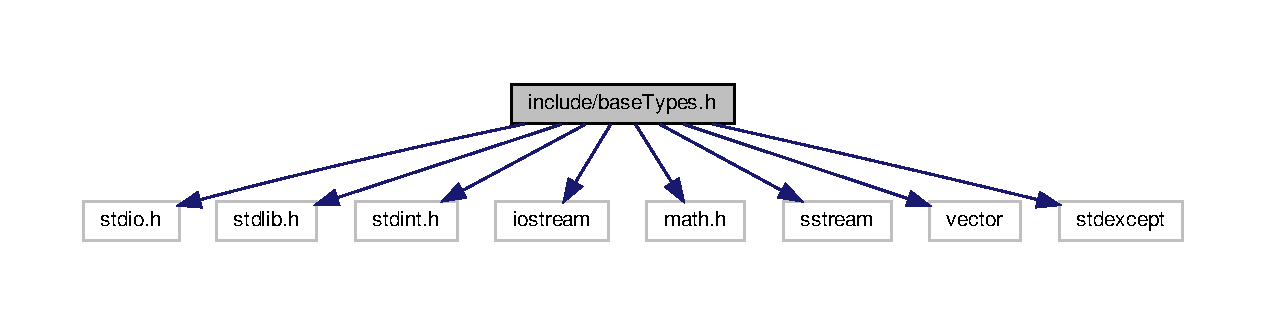
\includegraphics[width=350pt]{baseTypes_8h__incl}
\end{center}
\end{figure}
Este grafo mostra quais são os ficheiros que incluem directamente ou indirectamente este ficheiro\+:
\nopagebreak
\begin{figure}[H]
\begin{center}
\leavevmode
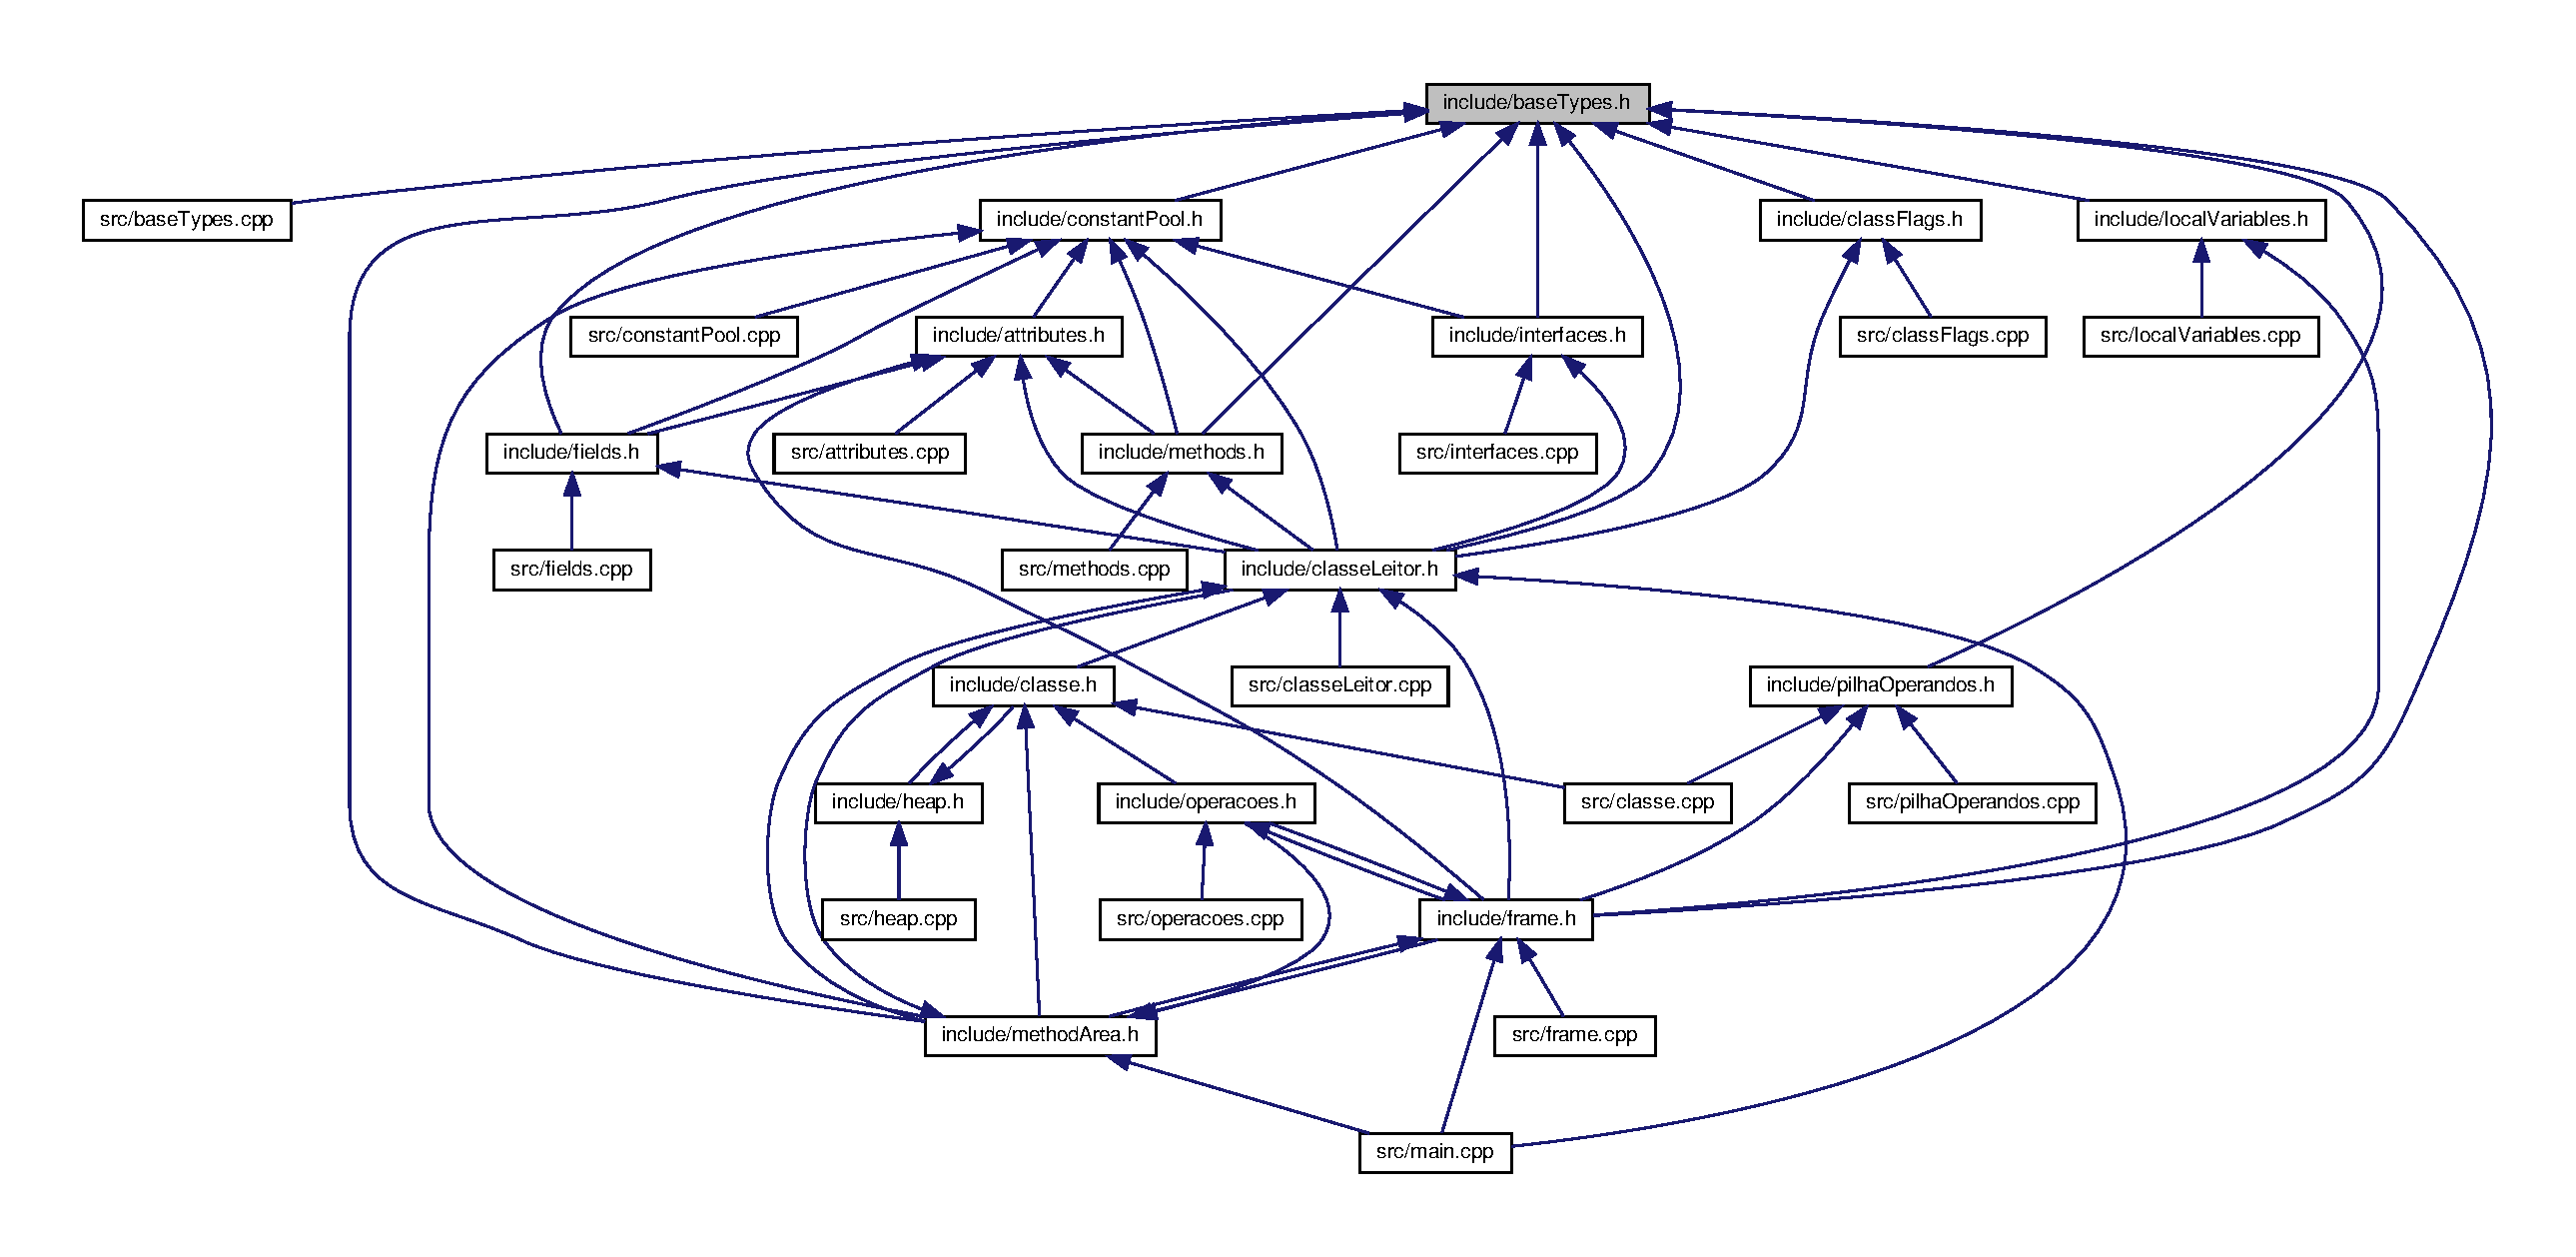
\includegraphics[width=350pt]{baseTypes_8h__dep__incl}
\end{center}
\end{figure}
\subsection*{Estruturas de Dados}
\begin{DoxyCompactItemize}
\item 
union \hyperlink{unionClassLoaderType}{Class\+Loader\+Type}
\begin{DoxyCompactList}\small\item\em Estrutura de dados para armazenamento Union responsável por armazenar todos os tamanhos de variáveis utilzadas na J\+VM. \end{DoxyCompactList}\item 
union \hyperlink{unionelement__u}{element\+\_\+u}
\begin{DoxyCompactList}\small\item\em Generalização de funções de retorno/input Union responsável pela generalização de funções de retorno e uma função de input. \end{DoxyCompactList}\item 
struct \hyperlink{structn__array}{n\+\_\+array}
\item 
struct \hyperlink{structtypedElement__s}{typed\+Element\+\_\+s}
\begin{DoxyCompactList}\small\item\em Agregador de tipos e informações. Struct responsável por juntar tipos e informações de elementos. \end{DoxyCompactList}\end{DoxyCompactItemize}
\subsection*{Macros}
\begin{DoxyCompactItemize}
\item 
\mbox{\Hypertarget{baseTypes_8h_a2222d817ce6bbd243023a7471e44a5d6}\label{baseTypes_8h_a2222d817ce6bbd243023a7471e44a5d6}} 
\#define {\bfseries Float\+\_\+\+NaN}~0x7f800001
\item 
\mbox{\Hypertarget{baseTypes_8h_af40742e3f905fd8d0968a3f0b5160649}\label{baseTypes_8h_af40742e3f905fd8d0968a3f0b5160649}} 
\#define {\bfseries Float\+\_\+\+Plus\+Infinity}~0x7f800000
\item 
\mbox{\Hypertarget{baseTypes_8h_a8553cea1fd99855eeadf2f4ea7a3ac72}\label{baseTypes_8h_a8553cea1fd99855eeadf2f4ea7a3ac72}} 
\#define {\bfseries Float\+\_\+\+Minus\+Infinity}~0xff800000
\item 
\mbox{\Hypertarget{baseTypes_8h_a30cf2596dc23460158fefbe6dc4c359e}\label{baseTypes_8h_a30cf2596dc23460158fefbe6dc4c359e}} 
\#define {\bfseries Double\+\_\+\+NaN}~0x7ff0000000000001L
\item 
\mbox{\Hypertarget{baseTypes_8h_a2323042af27da372d902198570438d6d}\label{baseTypes_8h_a2323042af27da372d902198570438d6d}} 
\#define {\bfseries Double\+\_\+\+Plus\+Infinity}~0x7ff0000000000000L
\item 
\mbox{\Hypertarget{baseTypes_8h_ad5fb6a3d0e63e11648c5f3ad7febb0ad}\label{baseTypes_8h_ad5fb6a3d0e63e11648c5f3ad7febb0ad}} 
\#define {\bfseries Double\+\_\+\+Minus\+Infinity}~0xfff0000000000000L
\item 
\mbox{\Hypertarget{baseTypes_8h_a5a991e148e312c68d851b11b4b7be584}\label{baseTypes_8h_a5a991e148e312c68d851b11b4b7be584}} 
\#define {\bfseries R\+T\+\_\+\+B\+Y\+TE}~1
\item 
\mbox{\Hypertarget{baseTypes_8h_ae0ecf90db844a032db00e19482c633d1}\label{baseTypes_8h_ae0ecf90db844a032db00e19482c633d1}} 
\#define {\bfseries R\+T\+\_\+\+B\+O\+OL}~2
\item 
\mbox{\Hypertarget{baseTypes_8h_aefa4685f803fc7df5788405390df6aab}\label{baseTypes_8h_aefa4685f803fc7df5788405390df6aab}} 
\#define {\bfseries R\+T\+\_\+\+C\+H\+AR}~3
\item 
\mbox{\Hypertarget{baseTypes_8h_a15a051a50ea712336d1e809ed5fe240f}\label{baseTypes_8h_a15a051a50ea712336d1e809ed5fe240f}} 
\#define {\bfseries R\+T\+\_\+\+S\+H\+O\+RT}~4
\item 
\mbox{\Hypertarget{baseTypes_8h_ae8d7be4292c8262f3fe8a12a9d5012f1}\label{baseTypes_8h_ae8d7be4292c8262f3fe8a12a9d5012f1}} 
\#define {\bfseries R\+T\+\_\+\+I\+NT}~5
\item 
\mbox{\Hypertarget{baseTypes_8h_a1eee60e646767c4b249177593302d237}\label{baseTypes_8h_a1eee60e646767c4b249177593302d237}} 
\#define {\bfseries R\+T\+\_\+\+F\+L\+O\+AT}~6
\item 
\mbox{\Hypertarget{baseTypes_8h_a3e1ffaf0d9c3d4614139871cfea4e779}\label{baseTypes_8h_a3e1ffaf0d9c3d4614139871cfea4e779}} 
\#define {\bfseries R\+T\+\_\+\+D\+O\+U\+B\+LE}~7
\item 
\mbox{\Hypertarget{baseTypes_8h_ac2620c935a093d64e17628fbb36a5e79}\label{baseTypes_8h_ac2620c935a093d64e17628fbb36a5e79}} 
\#define {\bfseries R\+T\+\_\+\+R\+E\+F\+E\+R\+E\+N\+CE}~8
\item 
\mbox{\Hypertarget{baseTypes_8h_a321c0fe6e16c9d74517df8a769fa723d}\label{baseTypes_8h_a321c0fe6e16c9d74517df8a769fa723d}} 
\#define {\bfseries R\+T\+\_\+\+L\+O\+NG}~9
\end{DoxyCompactItemize}
\subsection*{Definições de tipos}
\begin{DoxyCompactItemize}
\item 
\mbox{\Hypertarget{baseTypes_8h_a9bffe5bb2564f91cd90fb7d06848f9a8}\label{baseTypes_8h_a9bffe5bb2564f91cd90fb7d06848f9a8}} 
typedef uint8\+\_\+t {\bfseries U1}
\item 
\mbox{\Hypertarget{baseTypes_8h_a90240657108b1b457eef9d3f76e0202e}\label{baseTypes_8h_a90240657108b1b457eef9d3f76e0202e}} 
typedef uint16\+\_\+t {\bfseries U2}
\item 
\mbox{\Hypertarget{baseTypes_8h_ac6d2ba2e53dd424684ead2f40e74a8b6}\label{baseTypes_8h_ac6d2ba2e53dd424684ead2f40e74a8b6}} 
typedef uint32\+\_\+t {\bfseries U4}
\item 
\mbox{\Hypertarget{baseTypes_8h_a7413c5ade8aad8440eb5086c61173de5}\label{baseTypes_8h_a7413c5ade8aad8440eb5086c61173de5}} 
typedef union \hyperlink{unionelement__u}{element\+\_\+u} {\bfseries element}
\item 
\mbox{\Hypertarget{baseTypes_8h_a17b26383e038d1a85e30de17ddcb3292}\label{baseTypes_8h_a17b26383e038d1a85e30de17ddcb3292}} 
typedef struct \hyperlink{structtypedElement__s}{typed\+Element\+\_\+s} {\bfseries typed\+Element}
\end{DoxyCompactItemize}
\subsection*{Funções}
\begin{DoxyCompactItemize}
\item 
U1 \hyperlink{baseTypes_8h_a8a134c72da9699c32dbec57627955328}{read\+U1} (F\+I\+LE $\ast$fp)
\begin{DoxyCompactList}\small\item\em Função para ler 1 byte do arquivo .class. \end{DoxyCompactList}\item 
U2 \hyperlink{baseTypes_8h_a81f8cf10d3f1ee282c2f124ebf00b718}{read\+U2} (F\+I\+LE $\ast$fp)
\begin{DoxyCompactList}\small\item\em Função para ler 2 bytes do arquivo .class. \end{DoxyCompactList}\item 
U4 \hyperlink{baseTypes_8h_a836a4be80a9f428623a68e687e6c30c6}{read\+U4} (F\+I\+LE $\ast$fp)
\begin{DoxyCompactList}\small\item\em Função para ler 4 bytes do arquivo .class. \end{DoxyCompactList}\item 
U1 $\ast$ \hyperlink{baseTypes_8h_a1b1c1fe27d442689b07d0d54f17c44aa}{read\+U\+T\+F8} (F\+I\+LE $\ast$fp, int size)
\begin{DoxyCompactList}\small\item\em Função para ler os bytes de uma string U\+T\+F-\/8. \end{DoxyCompactList}\item 
string \hyperlink{baseTypes_8h_a22f1f8c2b398f9db39f18565b36986f1}{show\+U\+T\+F8} (unsigned char $\ast$s, int size)
\begin{DoxyCompactList}\small\item\em Função para montar e mostrar a uma string U\+T\+F-\/8. \end{DoxyCompactList}\item 
int \hyperlink{baseTypes_8h_a5acaa092b09c93a09a62a07642507b66}{check\+Float} (float)
\begin{DoxyCompactList}\small\item\em Função para verificar NaN e infinito. \end{DoxyCompactList}\item 
int \hyperlink{baseTypes_8h_a83beed8fe3725ef9da796d4fd5449346}{check\+Double} (double)
\begin{DoxyCompactList}\small\item\em Função para verificar NaN e infinito. \end{DoxyCompactList}\item 
string \hyperlink{baseTypes_8h_a2c059bd56e4f7b2f6f066c99def4c0a3}{float\+\_\+to\+\_\+string} (float)
\begin{DoxyCompactList}\small\item\em Função para converter float para string. \end{DoxyCompactList}\item 
string \hyperlink{baseTypes_8h_afb46c6880fb822cd896bd2365eb0f935}{double\+\_\+to\+\_\+string} (double)
\begin{DoxyCompactList}\small\item\em Função para converter double para string. \end{DoxyCompactList}\item 
float \hyperlink{baseTypes_8h_a0f3ffb86bcc68531d481dd68c556b086}{u4\+\_\+to\+\_\+float} (\hyperlink{unionClassLoaderType}{Class\+Loader\+Type} in)
\begin{DoxyCompactList}\small\item\em Function to convert 4 bytes to a float. \end{DoxyCompactList}\item 
long \hyperlink{baseTypes_8h_a5b4ee2146dd5beafbac7709a37bdbbd2}{u4\+\_\+to\+\_\+long} (\hyperlink{unionClassLoaderType}{Class\+Loader\+Type} high, \hyperlink{unionClassLoaderType}{Class\+Loader\+Type} low)
\begin{DoxyCompactList}\small\item\em Function to convert 8 bytes to a long. \end{DoxyCompactList}\item 
double \hyperlink{baseTypes_8h_a51bdc30e142e0a9d888eb56ce9b5484b}{u4\+\_\+to\+\_\+double} (\hyperlink{unionClassLoaderType}{Class\+Loader\+Type} high, \hyperlink{unionClassLoaderType}{Class\+Loader\+Type} low)
\begin{DoxyCompactList}\small\item\em Function to convert 8 bytes to a double. \end{DoxyCompactList}\end{DoxyCompactItemize}


\subsection{Descrição detalhada}
Tipos Base Tipos básicos utilizados para implementarmos a J\+VM. 



\subsection{Documentação das funções}
\mbox{\Hypertarget{baseTypes_8h_a83beed8fe3725ef9da796d4fd5449346}\label{baseTypes_8h_a83beed8fe3725ef9da796d4fd5449346}} 
\index{base\+Types.\+h@{base\+Types.\+h}!check\+Double@{check\+Double}}
\index{check\+Double@{check\+Double}!base\+Types.\+h@{base\+Types.\+h}}
\subsubsection{\texorpdfstring{check\+Double()}{checkDouble()}}
{\footnotesize\ttfamily int check\+Double (\begin{DoxyParamCaption}\item[{double}]{d }\end{DoxyParamCaption})}



Função para verificar NaN e infinito. 


\begin{DoxyParams}{Parâmetros}
{\em double} & Number to be checked. \\
\hline
\end{DoxyParams}
\mbox{\Hypertarget{baseTypes_8h_a5acaa092b09c93a09a62a07642507b66}\label{baseTypes_8h_a5acaa092b09c93a09a62a07642507b66}} 
\index{base\+Types.\+h@{base\+Types.\+h}!check\+Float@{check\+Float}}
\index{check\+Float@{check\+Float}!base\+Types.\+h@{base\+Types.\+h}}
\subsubsection{\texorpdfstring{check\+Float()}{checkFloat()}}
{\footnotesize\ttfamily int check\+Float (\begin{DoxyParamCaption}\item[{float}]{f }\end{DoxyParamCaption})}



Função para verificar NaN e infinito. 


\begin{DoxyParams}{Parâmetros}
{\em float} & Número a ser verificado. \\
\hline
\end{DoxyParams}
\mbox{\Hypertarget{baseTypes_8h_afb46c6880fb822cd896bd2365eb0f935}\label{baseTypes_8h_afb46c6880fb822cd896bd2365eb0f935}} 
\index{base\+Types.\+h@{base\+Types.\+h}!double\+\_\+to\+\_\+string@{double\+\_\+to\+\_\+string}}
\index{double\+\_\+to\+\_\+string@{double\+\_\+to\+\_\+string}!base\+Types.\+h@{base\+Types.\+h}}
\subsubsection{\texorpdfstring{double\+\_\+to\+\_\+string()}{double\_to\_string()}}
{\footnotesize\ttfamily string double\+\_\+to\+\_\+string (\begin{DoxyParamCaption}\item[{double}]{d }\end{DoxyParamCaption})}



Função para converter double para string. 


\begin{DoxyParams}{Parâmetros}
{\em double} & Número a ser convertido. \\
\hline
\end{DoxyParams}
\mbox{\Hypertarget{baseTypes_8h_a2c059bd56e4f7b2f6f066c99def4c0a3}\label{baseTypes_8h_a2c059bd56e4f7b2f6f066c99def4c0a3}} 
\index{base\+Types.\+h@{base\+Types.\+h}!float\+\_\+to\+\_\+string@{float\+\_\+to\+\_\+string}}
\index{float\+\_\+to\+\_\+string@{float\+\_\+to\+\_\+string}!base\+Types.\+h@{base\+Types.\+h}}
\subsubsection{\texorpdfstring{float\+\_\+to\+\_\+string()}{float\_to\_string()}}
{\footnotesize\ttfamily string float\+\_\+to\+\_\+string (\begin{DoxyParamCaption}\item[{float}]{f }\end{DoxyParamCaption})}



Função para converter float para string. 


\begin{DoxyParams}{Parâmetros}
{\em float} & Número a ser convertido. \\
\hline
\end{DoxyParams}
\mbox{\Hypertarget{baseTypes_8h_a8a134c72da9699c32dbec57627955328}\label{baseTypes_8h_a8a134c72da9699c32dbec57627955328}} 
\index{base\+Types.\+h@{base\+Types.\+h}!read\+U1@{read\+U1}}
\index{read\+U1@{read\+U1}!base\+Types.\+h@{base\+Types.\+h}}
\subsubsection{\texorpdfstring{read\+U1()}{readU1()}}
{\footnotesize\ttfamily U1 read\+U1 (\begin{DoxyParamCaption}\item[{F\+I\+LE $\ast$}]{fp }\end{DoxyParamCaption})}



Função para ler 1 byte do arquivo .class. 


\begin{DoxyParams}{Parâmetros}
{\em fp.} & Ponteiro pro arquivo .class \\
\hline
\end{DoxyParams}
\mbox{\Hypertarget{baseTypes_8h_a81f8cf10d3f1ee282c2f124ebf00b718}\label{baseTypes_8h_a81f8cf10d3f1ee282c2f124ebf00b718}} 
\index{base\+Types.\+h@{base\+Types.\+h}!read\+U2@{read\+U2}}
\index{read\+U2@{read\+U2}!base\+Types.\+h@{base\+Types.\+h}}
\subsubsection{\texorpdfstring{read\+U2()}{readU2()}}
{\footnotesize\ttfamily U2 read\+U2 (\begin{DoxyParamCaption}\item[{F\+I\+LE $\ast$}]{fp }\end{DoxyParamCaption})}



Função para ler 2 bytes do arquivo .class. 


\begin{DoxyParams}{Parâmetros}
{\em fp.} & Ponteiro pro arquivo .class \\
\hline
\end{DoxyParams}
\mbox{\Hypertarget{baseTypes_8h_a836a4be80a9f428623a68e687e6c30c6}\label{baseTypes_8h_a836a4be80a9f428623a68e687e6c30c6}} 
\index{base\+Types.\+h@{base\+Types.\+h}!read\+U4@{read\+U4}}
\index{read\+U4@{read\+U4}!base\+Types.\+h@{base\+Types.\+h}}
\subsubsection{\texorpdfstring{read\+U4()}{readU4()}}
{\footnotesize\ttfamily U4 read\+U4 (\begin{DoxyParamCaption}\item[{F\+I\+LE $\ast$}]{fp }\end{DoxyParamCaption})}



Função para ler 4 bytes do arquivo .class. 


\begin{DoxyParams}{Parâmetros}
{\em fp.} & Ponteiro pro arquivo .class \\
\hline
\end{DoxyParams}
\mbox{\Hypertarget{baseTypes_8h_a1b1c1fe27d442689b07d0d54f17c44aa}\label{baseTypes_8h_a1b1c1fe27d442689b07d0d54f17c44aa}} 
\index{base\+Types.\+h@{base\+Types.\+h}!read\+U\+T\+F8@{read\+U\+T\+F8}}
\index{read\+U\+T\+F8@{read\+U\+T\+F8}!base\+Types.\+h@{base\+Types.\+h}}
\subsubsection{\texorpdfstring{read\+U\+T\+F8()}{readUTF8()}}
{\footnotesize\ttfamily U1$\ast$ read\+U\+T\+F8 (\begin{DoxyParamCaption}\item[{F\+I\+LE $\ast$}]{fp,  }\item[{int}]{size }\end{DoxyParamCaption})}



Função para ler os bytes de uma string U\+T\+F-\/8. 


\begin{DoxyParams}{Parâmetros}
{\em fp.} & Ponteiro pro arquivo .class \\
\hline
{\em size} & Tamanho que será alocado para a string. \\
\hline
\end{DoxyParams}
\mbox{\Hypertarget{baseTypes_8h_a22f1f8c2b398f9db39f18565b36986f1}\label{baseTypes_8h_a22f1f8c2b398f9db39f18565b36986f1}} 
\index{base\+Types.\+h@{base\+Types.\+h}!show\+U\+T\+F8@{show\+U\+T\+F8}}
\index{show\+U\+T\+F8@{show\+U\+T\+F8}!base\+Types.\+h@{base\+Types.\+h}}
\subsubsection{\texorpdfstring{show\+U\+T\+F8()}{showUTF8()}}
{\footnotesize\ttfamily string show\+U\+T\+F8 (\begin{DoxyParamCaption}\item[{unsigned char $\ast$}]{s,  }\item[{int}]{size }\end{DoxyParamCaption})}



Função para montar e mostrar a uma string U\+T\+F-\/8. 


\begin{DoxyParams}{Parâmetros}
{\em s} & Ponteiro para a posição inicial de uam string Unicode. \\
\hline
{\em size} & Tamanho da string a ser impressa. \\
\hline
\end{DoxyParams}
\mbox{\Hypertarget{baseTypes_8h_a51bdc30e142e0a9d888eb56ce9b5484b}\label{baseTypes_8h_a51bdc30e142e0a9d888eb56ce9b5484b}} 
\index{base\+Types.\+h@{base\+Types.\+h}!u4\+\_\+to\+\_\+double@{u4\+\_\+to\+\_\+double}}
\index{u4\+\_\+to\+\_\+double@{u4\+\_\+to\+\_\+double}!base\+Types.\+h@{base\+Types.\+h}}
\subsubsection{\texorpdfstring{u4\+\_\+to\+\_\+double()}{u4\_to\_double()}}
{\footnotesize\ttfamily double u4\+\_\+to\+\_\+double (\begin{DoxyParamCaption}\item[{\hyperlink{unionClassLoaderType}{Class\+Loader\+Type}}]{high,  }\item[{\hyperlink{unionClassLoaderType}{Class\+Loader\+Type}}]{low }\end{DoxyParamCaption})}



Function to convert 8 bytes to a double. 


\begin{DoxyParams}{Parâmetros}
{\em high} & Four most significant bytes to be converted. \\
\hline
{\em low} & Four last significant bytes to be converted. \\
\hline
\end{DoxyParams}
\mbox{\Hypertarget{baseTypes_8h_a0f3ffb86bcc68531d481dd68c556b086}\label{baseTypes_8h_a0f3ffb86bcc68531d481dd68c556b086}} 
\index{base\+Types.\+h@{base\+Types.\+h}!u4\+\_\+to\+\_\+float@{u4\+\_\+to\+\_\+float}}
\index{u4\+\_\+to\+\_\+float@{u4\+\_\+to\+\_\+float}!base\+Types.\+h@{base\+Types.\+h}}
\subsubsection{\texorpdfstring{u4\+\_\+to\+\_\+float()}{u4\_to\_float()}}
{\footnotesize\ttfamily float u4\+\_\+to\+\_\+float (\begin{DoxyParamCaption}\item[{\hyperlink{unionClassLoaderType}{Class\+Loader\+Type}}]{in }\end{DoxyParamCaption})}



Function to convert 4 bytes to a float. 


\begin{DoxyParams}{Parâmetros}
{\em in} & Four bytes to be converted. \\
\hline
\end{DoxyParams}
\mbox{\Hypertarget{baseTypes_8h_a5b4ee2146dd5beafbac7709a37bdbbd2}\label{baseTypes_8h_a5b4ee2146dd5beafbac7709a37bdbbd2}} 
\index{base\+Types.\+h@{base\+Types.\+h}!u4\+\_\+to\+\_\+long@{u4\+\_\+to\+\_\+long}}
\index{u4\+\_\+to\+\_\+long@{u4\+\_\+to\+\_\+long}!base\+Types.\+h@{base\+Types.\+h}}
\subsubsection{\texorpdfstring{u4\+\_\+to\+\_\+long()}{u4\_to\_long()}}
{\footnotesize\ttfamily long u4\+\_\+to\+\_\+long (\begin{DoxyParamCaption}\item[{\hyperlink{unionClassLoaderType}{Class\+Loader\+Type}}]{high,  }\item[{\hyperlink{unionClassLoaderType}{Class\+Loader\+Type}}]{low }\end{DoxyParamCaption})}



Function to convert 8 bytes to a long. 


\begin{DoxyParams}{Parâmetros}
{\em high} & Four most significant bytes to be converted. \\
\hline
{\em low} & Four last significant bytes to be converted. \\
\hline
\end{DoxyParams}

\hypertarget{classe_8h}{}\section{Referência ao ficheiro include/classe.h}
\label{classe_8h}\index{include/classe.\+h@{include/classe.\+h}}


Definição da \hyperlink{classClasseEstatica}{Classe\+Estatica} e da \hyperlink{classClasseInstancia}{Classe\+Instancia}.  


{\ttfamily \#include \char`\"{}classe\+Leitor.\+h\char`\"{}}\newline
{\ttfamily \#include \char`\"{}heap.\+h\char`\"{}}\newline
{\ttfamily \#include $<$map$>$}\newline
Diagrama de dependências de inclusão para classe.\+h\+:\nopagebreak
\begin{figure}[H]
\begin{center}
\leavevmode
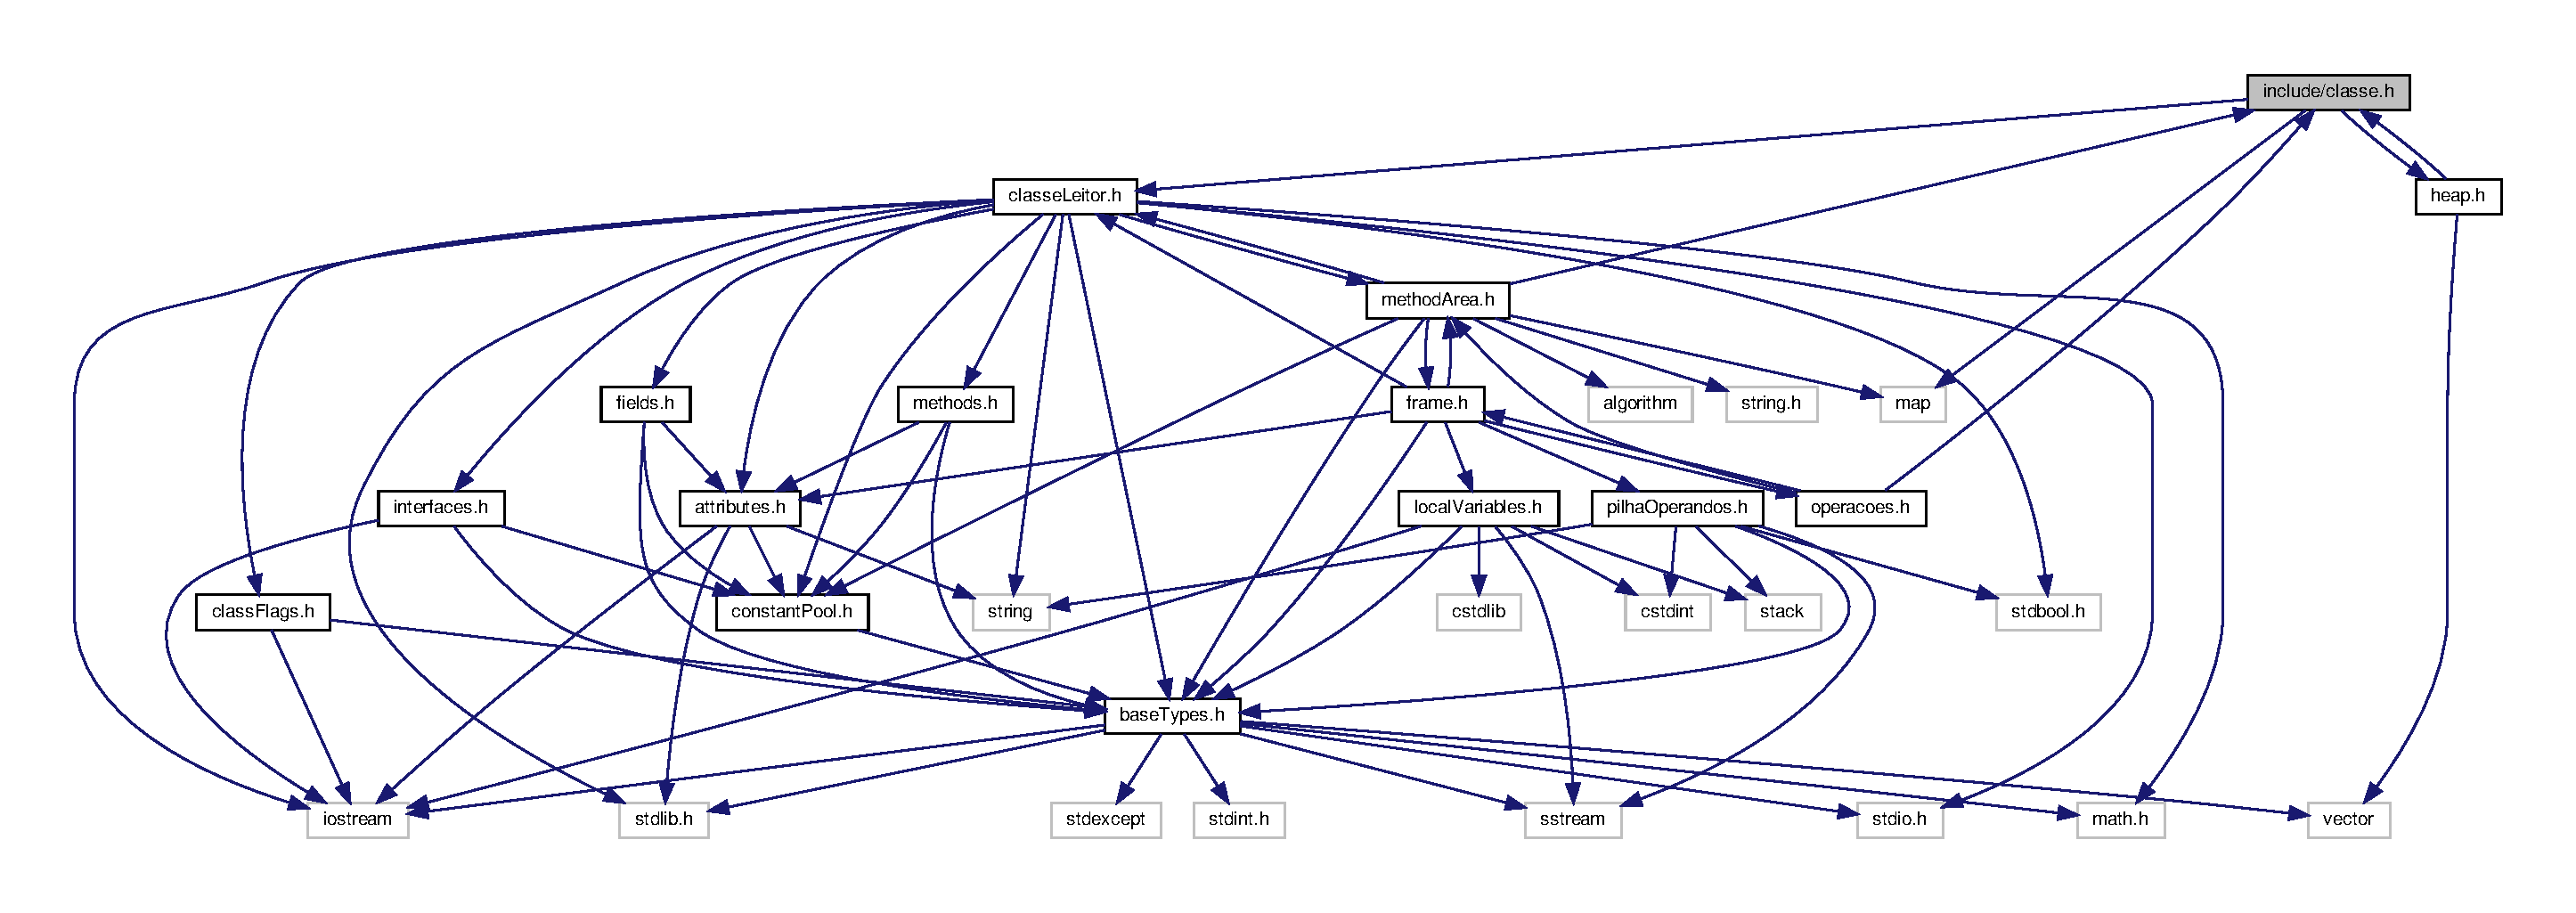
\includegraphics[width=350pt]{classe_8h__incl}
\end{center}
\end{figure}
Este grafo mostra quais são os ficheiros que incluem directamente ou indirectamente este ficheiro\+:\nopagebreak
\begin{figure}[H]
\begin{center}
\leavevmode
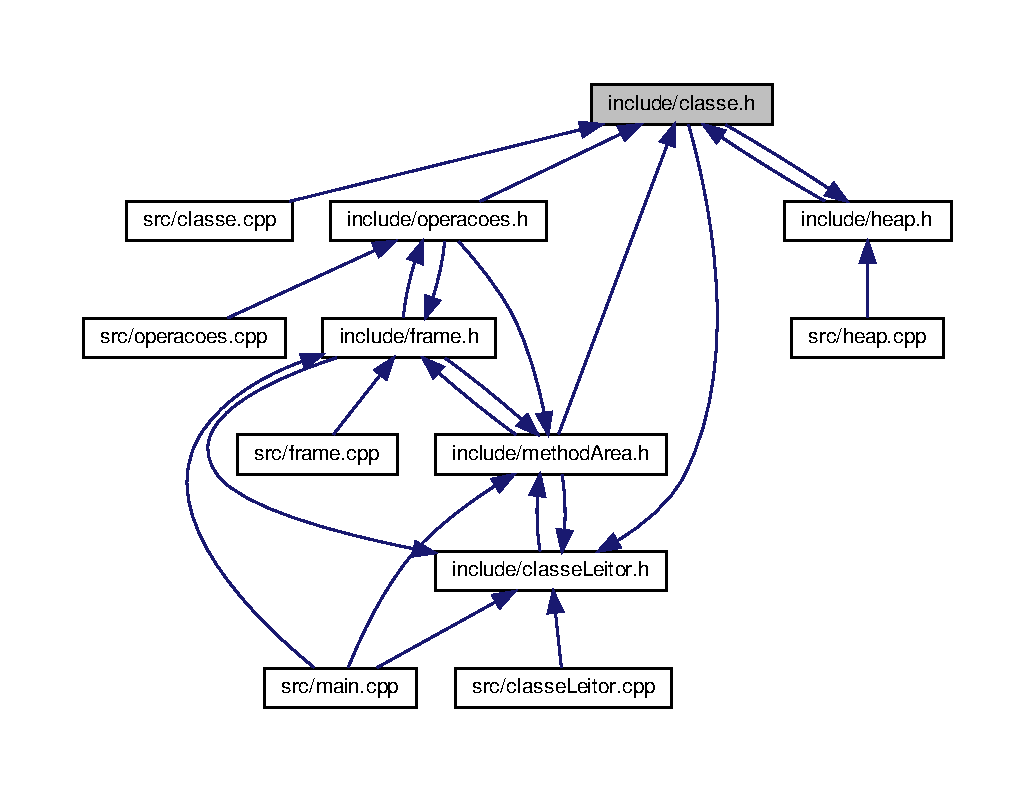
\includegraphics[width=350pt]{classe_8h__dep__incl}
\end{center}
\end{figure}
\subsection*{Estruturas de Dados}
\begin{DoxyCompactItemize}
\item 
class \hyperlink{classClasseEstatica}{Classe\+Estatica}
\begin{DoxyCompactList}\small\item\em Fields Estáticos compartilhados por todas as instâncias. \end{DoxyCompactList}\item 
class \hyperlink{classClasseInstancia}{Classe\+Instancia}
\begin{DoxyCompactList}\small\item\em Class instantiation. \end{DoxyCompactList}\end{DoxyCompactItemize}


\subsection{Descrição detalhada}
Definição da \hyperlink{classClasseEstatica}{Classe\+Estatica} e da \hyperlink{classClasseInstancia}{Classe\+Instancia}. 

Definição da Classe\+Leitor.
\hypertarget{classeLeitor_8h}{}\section{Referência ao ficheiro include/classe\+Leitor.h}
\label{classeLeitor_8h}\index{include/classe\+Leitor.\+h@{include/classe\+Leitor.\+h}}
{\ttfamily \#include $<$iostream$>$}\newline
{\ttfamily \#include $<$stdio.\+h$>$}\newline
{\ttfamily \#include $<$stdlib.\+h$>$}\newline
{\ttfamily \#include $<$math.\+h$>$}\newline
{\ttfamily \#include $<$stdbool.\+h$>$}\newline
{\ttfamily \#include $<$string$>$}\newline
{\ttfamily \#include \char`\"{}base\+Types.\+h\char`\"{}}\newline
{\ttfamily \#include \char`\"{}constant\+Pool.\+h\char`\"{}}\newline
{\ttfamily \#include \char`\"{}class\+Flags.\+h\char`\"{}}\newline
{\ttfamily \#include \char`\"{}fields.\+h\char`\"{}}\newline
{\ttfamily \#include \char`\"{}attributes.\+h\char`\"{}}\newline
{\ttfamily \#include \char`\"{}interfaces.\+h\char`\"{}}\newline
{\ttfamily \#include \char`\"{}methods.\+h\char`\"{}}\newline
{\ttfamily \#include \char`\"{}method\+Area.\+h\char`\"{}}\newline
Diagrama de dependências de inclusão para classe\+Leitor.\+h\+:
\nopagebreak
\begin{figure}[H]
\begin{center}
\leavevmode
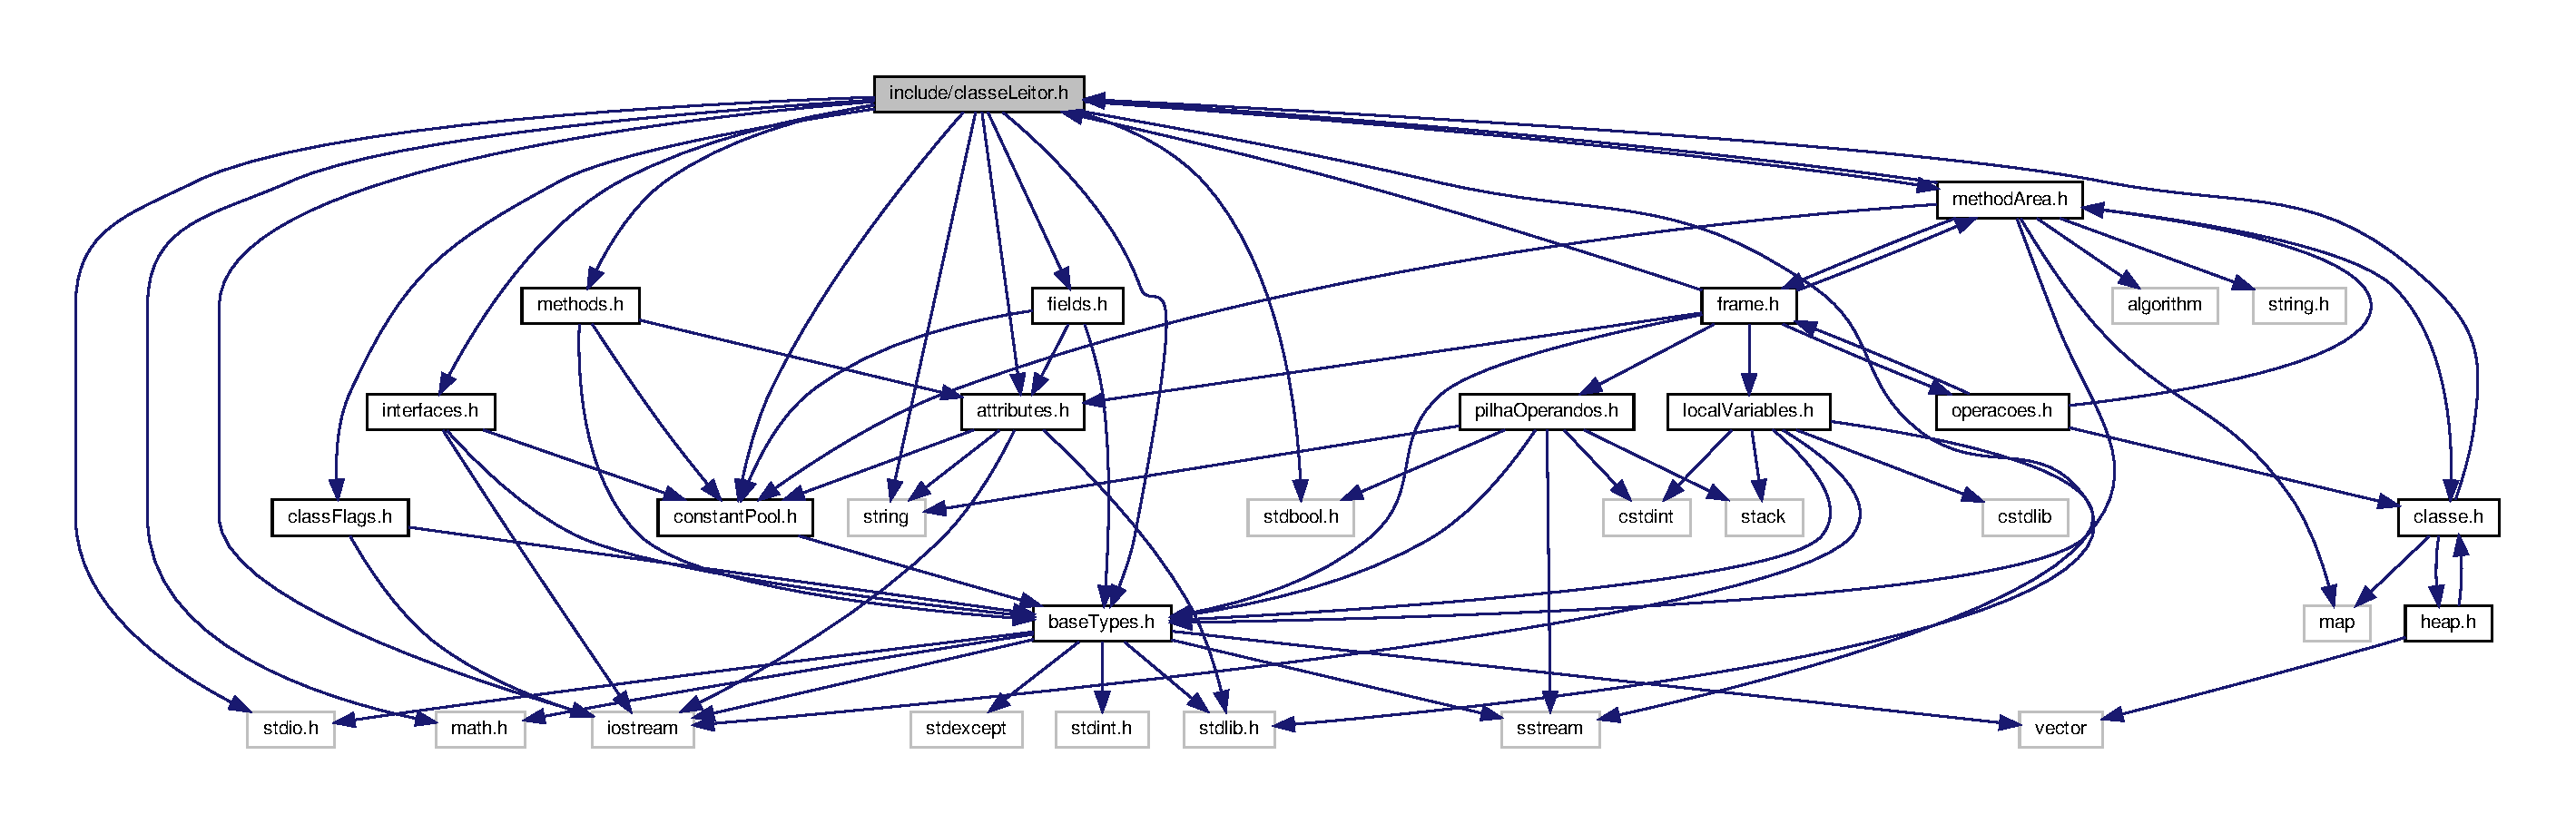
\includegraphics[width=350pt]{classeLeitor_8h__incl}
\end{center}
\end{figure}
Este grafo mostra quais são os ficheiros que incluem directamente ou indirectamente este ficheiro\+:
\nopagebreak
\begin{figure}[H]
\begin{center}
\leavevmode
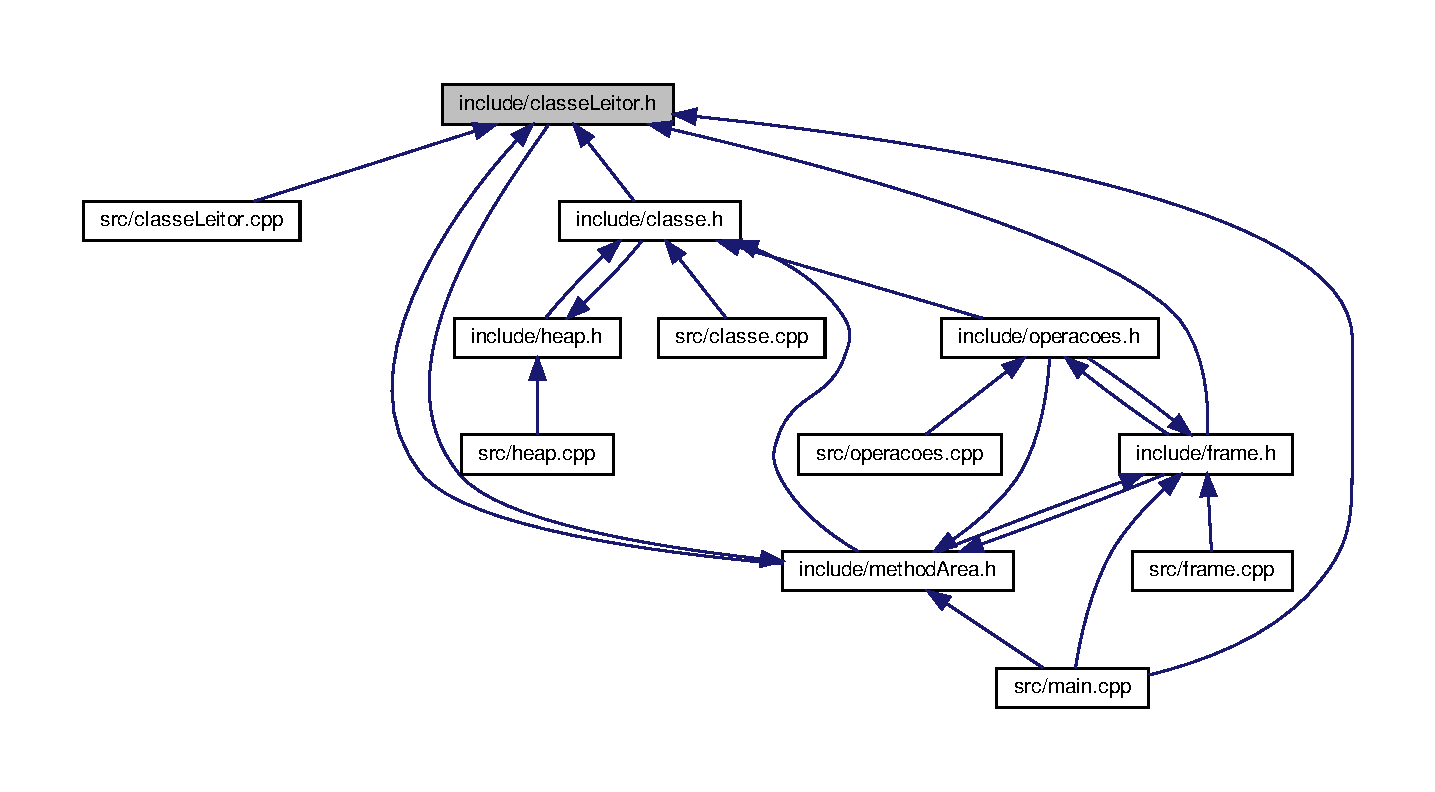
\includegraphics[width=350pt]{classeLeitor_8h__dep__incl}
\end{center}
\end{figure}
\subsection*{Estruturas de Dados}
\begin{DoxyCompactItemize}
\item 
class \hyperlink{classLeitor}{Leitor}
\end{DoxyCompactItemize}
\subsection*{Macros}
\begin{DoxyCompactItemize}
\item 
\#define \hyperlink{classeLeitor_8h_a3722a184bb01f895ee1bc5786cbefa8c}{M\+I\+S\+S\+I\+N\+G\+\_\+\+A\+R\+G\+U\+M\+E\+NT}~1
\item 
\mbox{\Hypertarget{classeLeitor_8h_aab73afd4d51f397415568f4a5fb80f6e}\label{classeLeitor_8h_aab73afd4d51f397415568f4a5fb80f6e}} 
\#define {\bfseries C\+A\+N\+T\+\_\+\+O\+P\+EN}~2
\item 
\mbox{\Hypertarget{classeLeitor_8h_a5f22fa59d1d8caa3fa4750147f559043}\label{classeLeitor_8h_a5f22fa59d1d8caa3fa4750147f559043}} 
\#define {\bfseries I\+N\+V\+A\+L\+I\+D\+\_\+\+F\+I\+LE}~3
\item 
\mbox{\Hypertarget{classeLeitor_8h_a2d08587be7624f46d6e1ce0892ab3ad4}\label{classeLeitor_8h_a2d08587be7624f46d6e1ce0892ab3ad4}} 
\#define {\bfseries U\+N\+K\+N\+O\+W\+N\+\_\+\+T\+Y\+PE}~4
\item 
\mbox{\Hypertarget{classeLeitor_8h_a0122e6d8e9f62e0e7d20a6d2ef7a4714}\label{classeLeitor_8h_a0122e6d8e9f62e0e7d20a6d2ef7a4714}} 
\#define {\bfseries I\+N\+V\+A\+L\+I\+D\+\_\+\+N\+A\+ME}~5
\item 
\mbox{\Hypertarget{classeLeitor_8h_a98e3929e6949250eb69f579b5fa83f3d}\label{classeLeitor_8h_a98e3929e6949250eb69f579b5fa83f3d}} 
\#define {\bfseries I\+N\+V\+A\+L\+I\+D\+\_\+\+E\+X\+T\+E\+N\+S\+I\+ON}~6
\item 
\mbox{\Hypertarget{classeLeitor_8h_a02b051cf9a5b88d508a6abe525221e37}\label{classeLeitor_8h_a02b051cf9a5b88d508a6abe525221e37}} 
\#define {\bfseries M\+I\+S\+S\+I\+N\+G\+\_\+\+M\+A\+IN}~7
\end{DoxyCompactItemize}


\subsection{Descrição detalhada}
\begin{DoxyAuthor}{Autor}
Bruno Cordeiro 
\end{DoxyAuthor}
\begin{DoxyVersion}{Versão}
1.\+0
\end{DoxyVersion}
\hypertarget{classeLeitor_8h_DESCRIPTION}{}\subsection{D\+E\+S\+C\+R\+I\+P\+T\+I\+ON}\label{classeLeitor_8h_DESCRIPTION}
A classe \hyperlink{classLeitor}{Leitor} contém o necessário para ler o bytecode, exibilo e armazena-\/lo em memoria 

\subsection{Documentação das macros}
\mbox{\Hypertarget{classeLeitor_8h_a3722a184bb01f895ee1bc5786cbefa8c}\label{classeLeitor_8h_a3722a184bb01f895ee1bc5786cbefa8c}} 
\index{classe\+Leitor.\+h@{classe\+Leitor.\+h}!M\+I\+S\+S\+I\+N\+G\+\_\+\+A\+R\+G\+U\+M\+E\+NT@{M\+I\+S\+S\+I\+N\+G\+\_\+\+A\+R\+G\+U\+M\+E\+NT}}
\index{M\+I\+S\+S\+I\+N\+G\+\_\+\+A\+R\+G\+U\+M\+E\+NT@{M\+I\+S\+S\+I\+N\+G\+\_\+\+A\+R\+G\+U\+M\+E\+NT}!classe\+Leitor.\+h@{classe\+Leitor.\+h}}
\subsubsection{\texorpdfstring{M\+I\+S\+S\+I\+N\+G\+\_\+\+A\+R\+G\+U\+M\+E\+NT}{MISSING\_ARGUMENT}}
{\footnotesize\ttfamily \#define M\+I\+S\+S\+I\+N\+G\+\_\+\+A\+R\+G\+U\+M\+E\+NT~1}

M\+A\+C\+R\+OS para os possíves erros encontrados 
\hypertarget{classFlags_8h}{}\section{Referência ao ficheiro include/class\+Flags.h}
\label{classFlags_8h}\index{include/class\+Flags.\+h@{include/class\+Flags.\+h}}


Class Flags.  


{\ttfamily \#include $<$iostream$>$}\newline
{\ttfamily \#include \char`\"{}base\+Types.\+h\char`\"{}}\newline
Diagrama de dependências de inclusão para class\+Flags.\+h\+:\nopagebreak
\begin{figure}[H]
\begin{center}
\leavevmode
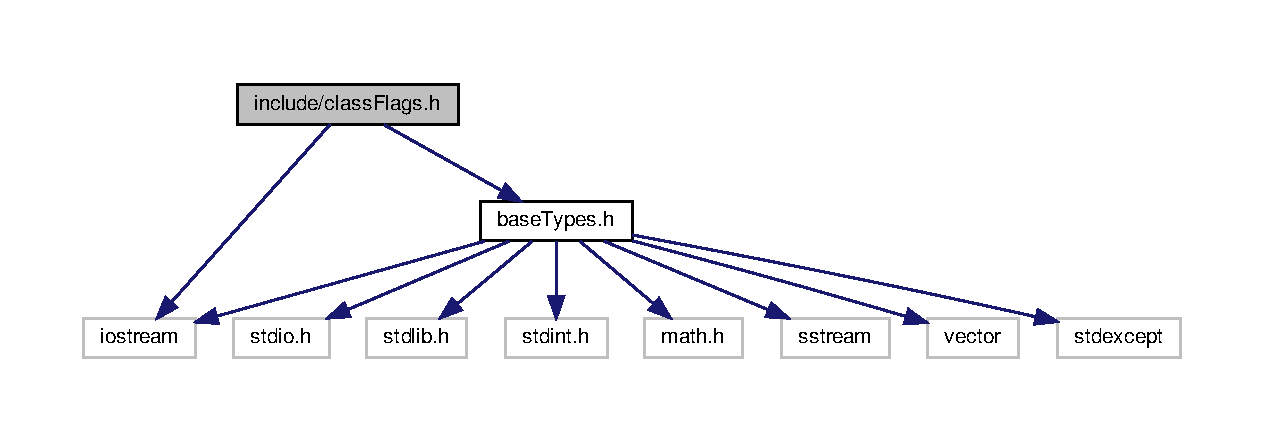
\includegraphics[width=350pt]{classFlags_8h__incl}
\end{center}
\end{figure}
Este grafo mostra quais são os ficheiros que incluem directamente ou indirectamente este ficheiro\+:\nopagebreak
\begin{figure}[H]
\begin{center}
\leavevmode
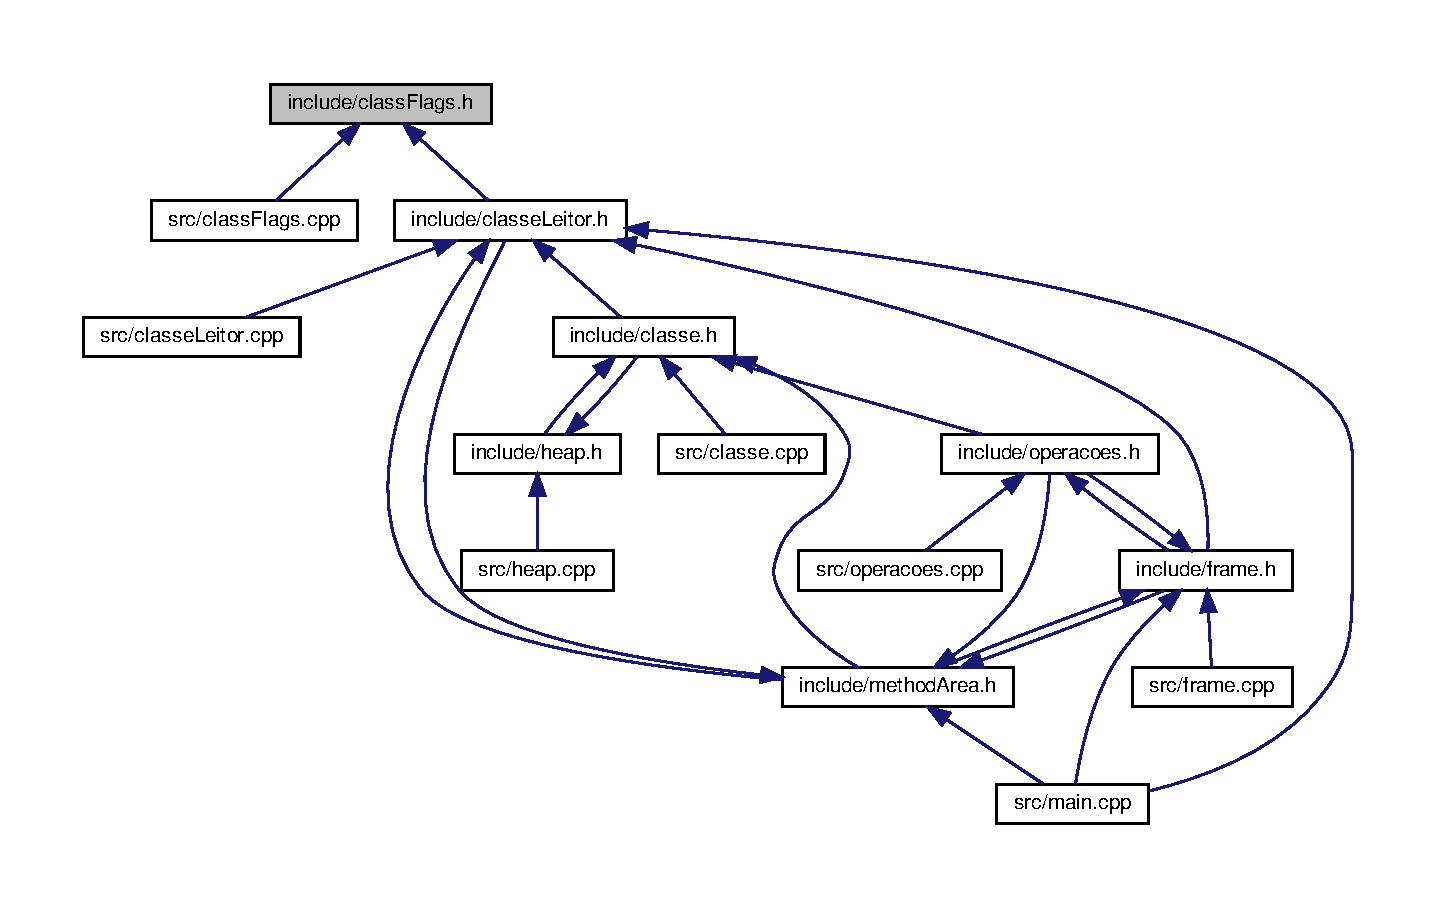
\includegraphics[width=350pt]{classFlags_8h__dep__incl}
\end{center}
\end{figure}
\subsection*{Funções}
\begin{DoxyCompactItemize}
\item 
void \hyperlink{classFlags_8h_a730d453861fb0b1e132ce23626a9dd98}{show\+Flags} (U2 flags)
\begin{DoxyCompactList}\small\item\em Função que mostra as flags de acesso para os usuários. \end{DoxyCompactList}\end{DoxyCompactItemize}
\subsection*{Variáveis}
\begin{DoxyCompactItemize}
\item 
\mbox{\Hypertarget{classFlags_8h_a3f0f33b3a86ad44099b106509ef17132}\label{classFlags_8h_a3f0f33b3a86ad44099b106509ef17132}} 
const string {\bfseries flag\+Names} \mbox{[}$\,$\mbox{]} = \{\char`\"{}A\+C\+C\+\_\+\+P\+U\+B\+L\+IC\char`\"{}, \char`\"{}A\+C\+C\+\_\+\+F\+I\+N\+AL\char`\"{}, \char`\"{}A\+C\+C\+\_\+\+S\+U\+P\+ER\char`\"{}, \char`\"{}A\+C\+C\+\_\+\+I\+N\+T\+E\+R\+F\+A\+CE\char`\"{}, \char`\"{}A\+C\+C\+\_\+\+A\+B\+S\+T\+R\+A\+CT\char`\"{}\}
\end{DoxyCompactItemize}


\subsection{Descrição detalhada}
Class Flags. 

Class\+Flags (public, final, super, interface and abstract) 

\subsection{Documentação das funções}
\mbox{\Hypertarget{classFlags_8h_a730d453861fb0b1e132ce23626a9dd98}\label{classFlags_8h_a730d453861fb0b1e132ce23626a9dd98}} 
\index{class\+Flags.\+h@{class\+Flags.\+h}!show\+Flags@{show\+Flags}}
\index{show\+Flags@{show\+Flags}!class\+Flags.\+h@{class\+Flags.\+h}}
\subsubsection{\texorpdfstring{show\+Flags()}{showFlags()}}
{\footnotesize\ttfamily void show\+Flags (\begin{DoxyParamCaption}\item[{U2}]{access\+Flags }\end{DoxyParamCaption})}



Função que mostra as flags de acesso para os usuários. 

Função que mostra as flags de acesso para os usuários 
\begin{DoxyParams}{Parâmetros}
{\em flags} & Valor hexadecimal das flags\\
\hline
{\em flags} & Valor hexadecimal das flags \\
\hline
\end{DoxyParams}

\hypertarget{constantPool_8h}{}\section{Referência ao ficheiro include/constant\+Pool.h}
\label{constantPool_8h}\index{include/constant\+Pool.\+h@{include/constant\+Pool.\+h}}


Módulo Constant pool.  


{\ttfamily \#include \char`\"{}base\+Types.\+h\char`\"{}}\newline
Diagrama de dependências de inclusão para constant\+Pool.\+h\+:
\nopagebreak
\begin{figure}[H]
\begin{center}
\leavevmode
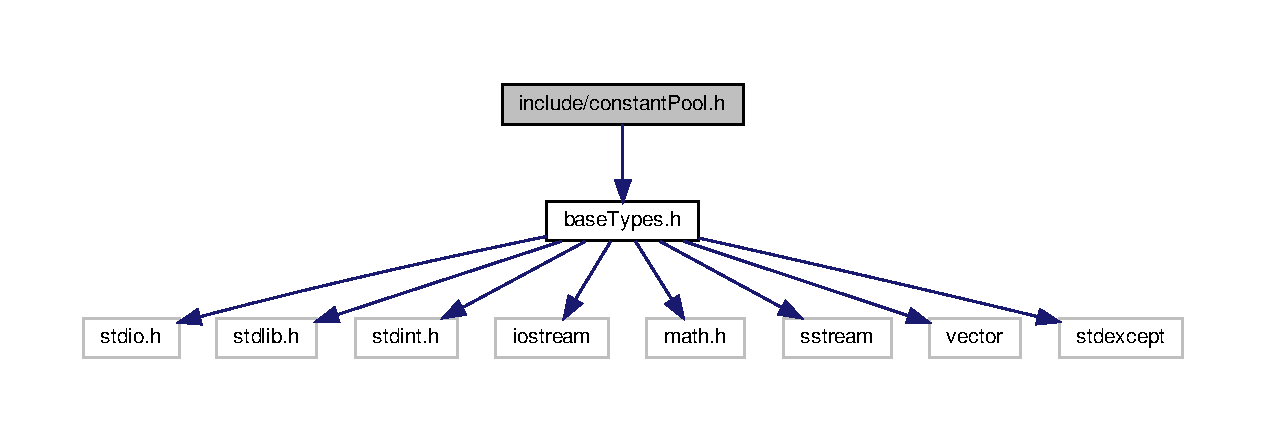
\includegraphics[width=350pt]{constantPool_8h__incl}
\end{center}
\end{figure}
Este grafo mostra quais são os ficheiros que incluem directamente ou indirectamente este ficheiro\+:
\nopagebreak
\begin{figure}[H]
\begin{center}
\leavevmode
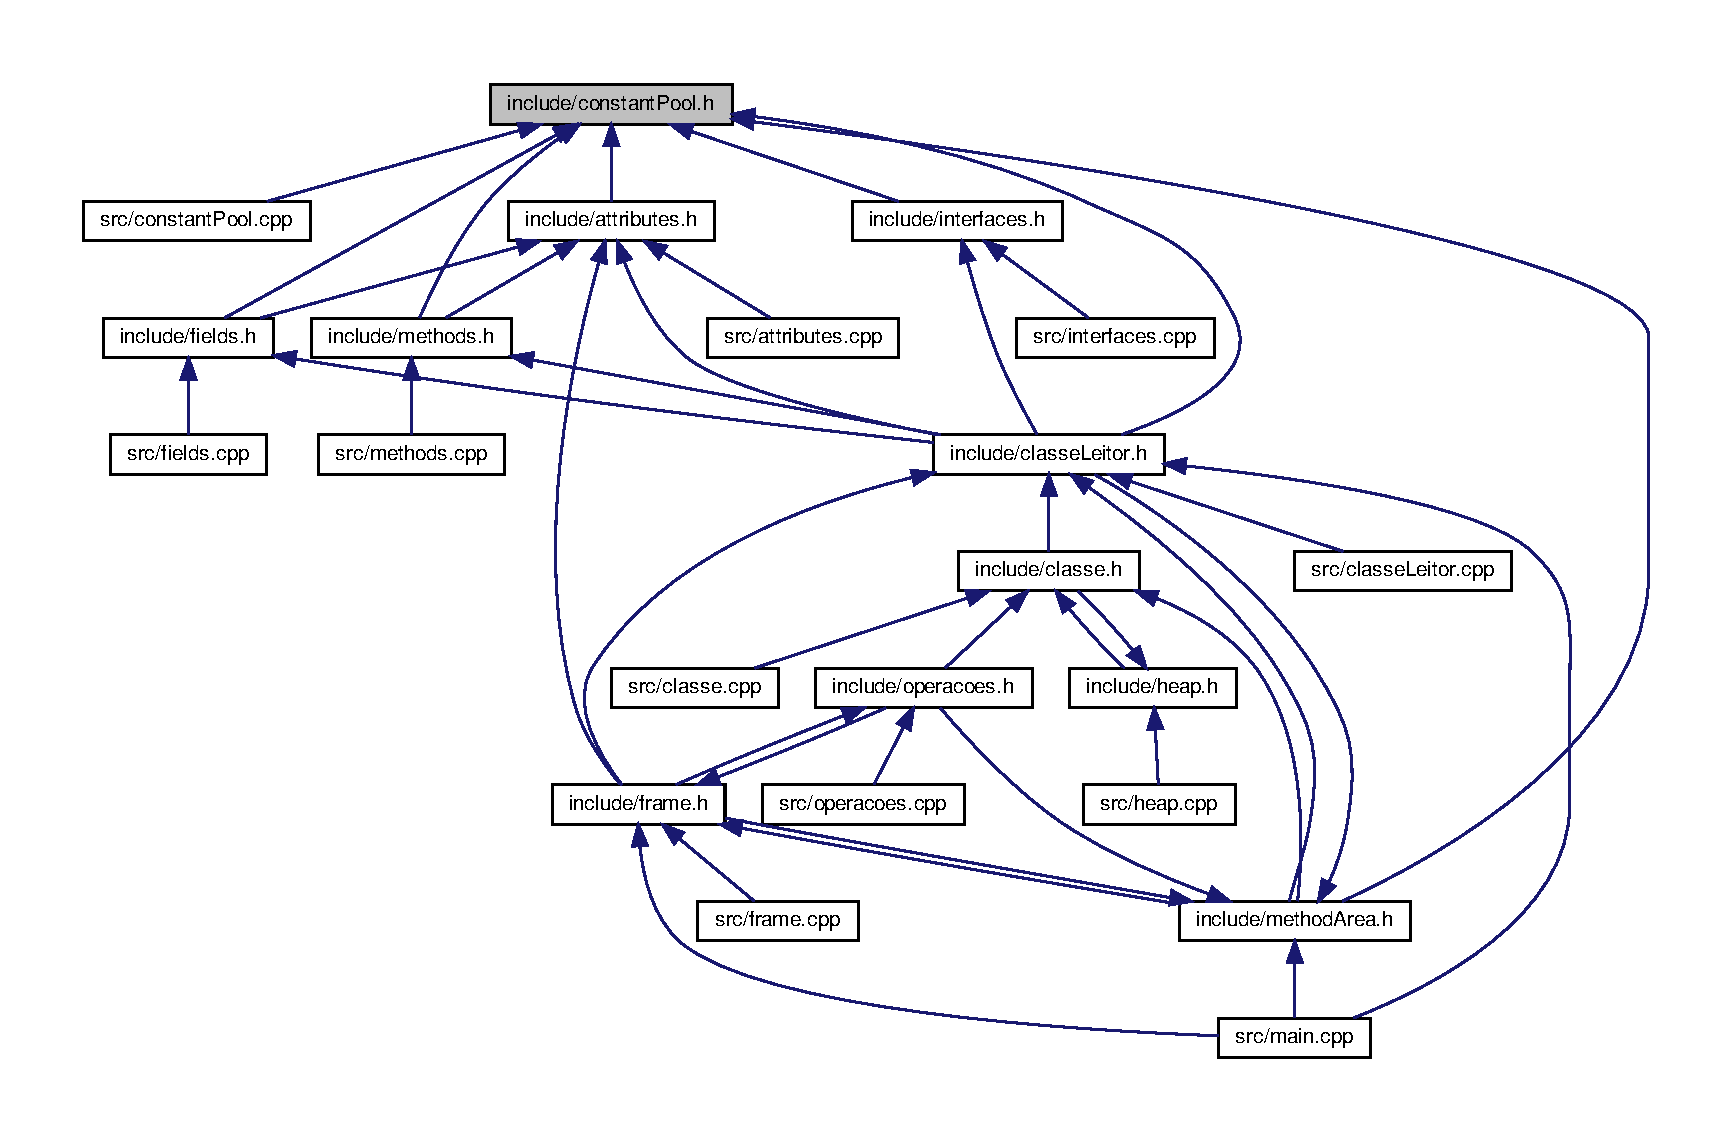
\includegraphics[width=350pt]{constantPool_8h__dep__incl}
\end{center}
\end{figure}
\subsection*{Estruturas de Dados}
\begin{DoxyCompactItemize}
\item 
struct \hyperlink{structcp__info}{cp\+\_\+info}
\begin{DoxyCompactList}\small\item\em Possui um elemento pool de constante. \end{DoxyCompactList}\end{DoxyCompactItemize}
\subsection*{Macros}
\begin{DoxyCompactItemize}
\item 
\mbox{\Hypertarget{constantPool_8h_adf770fe2eec438e3758ffe905dbae208}\label{constantPool_8h_adf770fe2eec438e3758ffe905dbae208}} 
\#define {\bfseries I\+N\+V\+A\+L\+ID}~99
\item 
\mbox{\Hypertarget{constantPool_8h_af9a8bd70343e082dbc63ac806b8ced24}\label{constantPool_8h_af9a8bd70343e082dbc63ac806b8ced24}} 
\#define {\bfseries U\+T\+F8}~1
\item 
\mbox{\Hypertarget{constantPool_8h_a91d43eadec33c80149f92e5abf5df58c}\label{constantPool_8h_a91d43eadec33c80149f92e5abf5df58c}} 
\#define {\bfseries I\+N\+T\+E\+G\+ER}~3
\item 
\mbox{\Hypertarget{constantPool_8h_ae8690abbffa85934d64d545920e2b108}\label{constantPool_8h_ae8690abbffa85934d64d545920e2b108}} 
\#define {\bfseries F\+L\+O\+AT}~4
\item 
\mbox{\Hypertarget{constantPool_8h_acaa7b8a7167a8214f499c71c413ddcca}\label{constantPool_8h_acaa7b8a7167a8214f499c71c413ddcca}} 
\#define {\bfseries L\+O\+NG}~5
\item 
\mbox{\Hypertarget{constantPool_8h_a8747af38b86aa2bbcda2f1b1aa0888c2}\label{constantPool_8h_a8747af38b86aa2bbcda2f1b1aa0888c2}} 
\#define {\bfseries D\+O\+U\+B\+LE}~6
\item 
\mbox{\Hypertarget{constantPool_8h_aeb04f2e0012cb07d68538599161c9693}\label{constantPool_8h_aeb04f2e0012cb07d68538599161c9693}} 
\#define {\bfseries C\+L\+A\+SS}~7
\item 
\mbox{\Hypertarget{constantPool_8h_a0f4d394a3ab4e09bff60f714c66dc5ee}\label{constantPool_8h_a0f4d394a3ab4e09bff60f714c66dc5ee}} 
\#define {\bfseries S\+T\+R\+I\+NG}~8
\item 
\mbox{\Hypertarget{constantPool_8h_a961f6036be890ad905abf769f04099fb}\label{constantPool_8h_a961f6036be890ad905abf769f04099fb}} 
\#define {\bfseries F\+I\+E\+L\+D\+\_\+\+R\+EF}~9
\item 
\mbox{\Hypertarget{constantPool_8h_a4bb1d2e6bfe342f8f25c01e8feab94f6}\label{constantPool_8h_a4bb1d2e6bfe342f8f25c01e8feab94f6}} 
\#define {\bfseries M\+E\+T\+H\+O\+D\+\_\+\+R\+EF}~10
\item 
\mbox{\Hypertarget{constantPool_8h_a192895ca38ee080d81750923e92639db}\label{constantPool_8h_a192895ca38ee080d81750923e92639db}} 
\#define {\bfseries I\+N\+T\+E\+R\+F\+A\+C\+E\+\_\+\+R\+EF}~11
\item 
\mbox{\Hypertarget{constantPool_8h_ab69e20acf60d75560d828fd8e89d8a39}\label{constantPool_8h_ab69e20acf60d75560d828fd8e89d8a39}} 
\#define {\bfseries N\+A\+M\+E\+\_\+\+A\+N\+D\+\_\+\+T\+Y\+PE}~12
\end{DoxyCompactItemize}
\subsection*{Funções}
\begin{DoxyCompactItemize}
\item 
int \hyperlink{constantPool_8h_aeed51c70547d5b043643766a20b34127}{load\+Constant\+Pool} (\hyperlink{structcp__info}{cp\+\_\+info} $\ast$constant\+Pool, int length\+CP, F\+I\+LE $\ast$fp)
\begin{DoxyCompactList}\small\item\em Carrega o pool de constantes. \end{DoxyCompactList}\item 
string \hyperlink{constantPool_8h_a3b41d9a03a7d0060e40c3135a4d341b9}{dereference\+Index} (\hyperlink{structcp__info}{cp\+\_\+info} $\ast$cp, U2 index)
\begin{DoxyCompactList}\small\item\em Retorna os dados no índice. \end{DoxyCompactList}\item 
void \hyperlink{constantPool_8h_a885fc96896e2694a220fb936c97b929f}{print\+Constant\+Pool} (\hyperlink{structcp__info}{cp\+\_\+info} $\ast$constant\+Pool, int length\+CP)
\begin{DoxyCompactList}\small\item\em Imprime o pool de constantes. \end{DoxyCompactList}\end{DoxyCompactItemize}
\subsection*{Variáveis}
\begin{DoxyCompactItemize}
\item 
\mbox{\Hypertarget{constantPool_8h_aabf3d9e746ea5b69b031bd8eb1a71421}\label{constantPool_8h_aabf3d9e746ea5b69b031bd8eb1a71421}} 
const string \hyperlink{constantPool_8h_aabf3d9e746ea5b69b031bd8eb1a71421}{type\+Names} \mbox{[}$\,$\mbox{]} = \{\char`\"{}U\+TF-\/8\char`\"{}, \char`\"{}-\/\char`\"{}, \char`\"{}Integer\char`\"{}, \char`\"{}Float\char`\"{}, \char`\"{}Long\char`\"{}, \char`\"{}Double\char`\"{}, \char`\"{}Class\char`\"{}, \char`\"{}String\char`\"{}, \char`\"{}Field\char`\"{}, \char`\"{}Method\char`\"{}, \char`\"{}Interface\char`\"{}, \char`\"{}Name and Type\char`\"{}\}
\begin{DoxyCompactList}\small\item\em Formatos de dados no pool de constantes. \end{DoxyCompactList}\end{DoxyCompactItemize}


\subsection{Descrição detalhada}
Módulo Constant pool. 

Este módulo contém as funções necessárias para a manipulação do pool de constantes. 

\subsection{Documentação das funções}
\mbox{\Hypertarget{constantPool_8h_a3b41d9a03a7d0060e40c3135a4d341b9}\label{constantPool_8h_a3b41d9a03a7d0060e40c3135a4d341b9}} 
\index{constant\+Pool.\+h@{constant\+Pool.\+h}!dereference\+Index@{dereference\+Index}}
\index{dereference\+Index@{dereference\+Index}!constant\+Pool.\+h@{constant\+Pool.\+h}}
\subsubsection{\texorpdfstring{dereference\+Index()}{dereferenceIndex()}}
{\footnotesize\ttfamily string dereference\+Index (\begin{DoxyParamCaption}\item[{\hyperlink{structcp__info}{cp\+\_\+info} $\ast$}]{cp,  }\item[{U2}]{index }\end{DoxyParamCaption})}



Retorna os dados no índice. 


\begin{DoxyParams}{Parâmetros}
{\em cp} & -\/ um ponteiro para o pool de contantes \\
\hline
{\em index} & -\/ um índice para a posição no pool de constantes \\
\hline
\end{DoxyParams}
\hypertarget{constantPool_8cpp_desc}{}\subsection{Descrição}\label{constantPool_8cpp_desc}
Função responsável por obter os dados correspondentes ao índice informado \mbox{\Hypertarget{constantPool_8h_aeed51c70547d5b043643766a20b34127}\label{constantPool_8h_aeed51c70547d5b043643766a20b34127}} 
\index{constant\+Pool.\+h@{constant\+Pool.\+h}!load\+Constant\+Pool@{load\+Constant\+Pool}}
\index{load\+Constant\+Pool@{load\+Constant\+Pool}!constant\+Pool.\+h@{constant\+Pool.\+h}}
\subsubsection{\texorpdfstring{load\+Constant\+Pool()}{loadConstantPool()}}
{\footnotesize\ttfamily int load\+Constant\+Pool (\begin{DoxyParamCaption}\item[{\hyperlink{structcp__info}{cp\+\_\+info} $\ast$}]{constant\+Pool,  }\item[{int}]{length\+CP,  }\item[{F\+I\+LE $\ast$}]{fp }\end{DoxyParamCaption})}



Carrega o pool de constantes. 


\begin{DoxyParams}{Parâmetros}
{\em constant\+Pool} & -\/ um ponteiro para o pool de contantes \\
\hline
{\em length\+CP} & -\/ o tamanho do pool de constantes \\
\hline
{\em fp} & -\/ ponteiro para o arquivo .class \\
\hline
\end{DoxyParams}
\hypertarget{constantPool_8cpp_desc}{}\subsection{Descrição}\label{constantPool_8cpp_desc}
Função responsável por carregar o pool de constantes e todos os campos a ele relacionados \begin{DoxyReturn}{Retorna}
o número de elementos do pool de constantes 
\end{DoxyReturn}
\mbox{\Hypertarget{constantPool_8h_a885fc96896e2694a220fb936c97b929f}\label{constantPool_8h_a885fc96896e2694a220fb936c97b929f}} 
\index{constant\+Pool.\+h@{constant\+Pool.\+h}!print\+Constant\+Pool@{print\+Constant\+Pool}}
\index{print\+Constant\+Pool@{print\+Constant\+Pool}!constant\+Pool.\+h@{constant\+Pool.\+h}}
\subsubsection{\texorpdfstring{print\+Constant\+Pool()}{printConstantPool()}}
{\footnotesize\ttfamily void print\+Constant\+Pool (\begin{DoxyParamCaption}\item[{\hyperlink{structcp__info}{cp\+\_\+info} $\ast$}]{constant\+Pool,  }\item[{int}]{length\+CP }\end{DoxyParamCaption})}



Imprime o pool de constantes. 


\begin{DoxyParams}{Parâmetros}
{\em constant\+Pool} & -\/ um ponteiro para o pool de contantes \\
\hline
{\em length\+CP} & -\/ o tamanho do pool de constantes \\
\hline
\end{DoxyParams}
\hypertarget{constantPool_8cpp_desc}{}\subsection{Descrição}\label{constantPool_8cpp_desc}
Função responsável por imprimir na tela o pool de constantes e todos os campos a ele relacionados 
\hypertarget{fields_8h}{}\section{Referência ao ficheiro include/fields.h}
\label{fields_8h}\index{include/fields.\+h@{include/fields.\+h}}


Classe field.  


{\ttfamily \#include \char`\"{}base\+Types.\+h\char`\"{}}\newline
{\ttfamily \#include \char`\"{}constant\+Pool.\+h\char`\"{}}\newline
{\ttfamily \#include \char`\"{}attributes.\+h\char`\"{}}\newline
Diagrama de dependências de inclusão para fields.\+h\+:\nopagebreak
\begin{figure}[H]
\begin{center}
\leavevmode
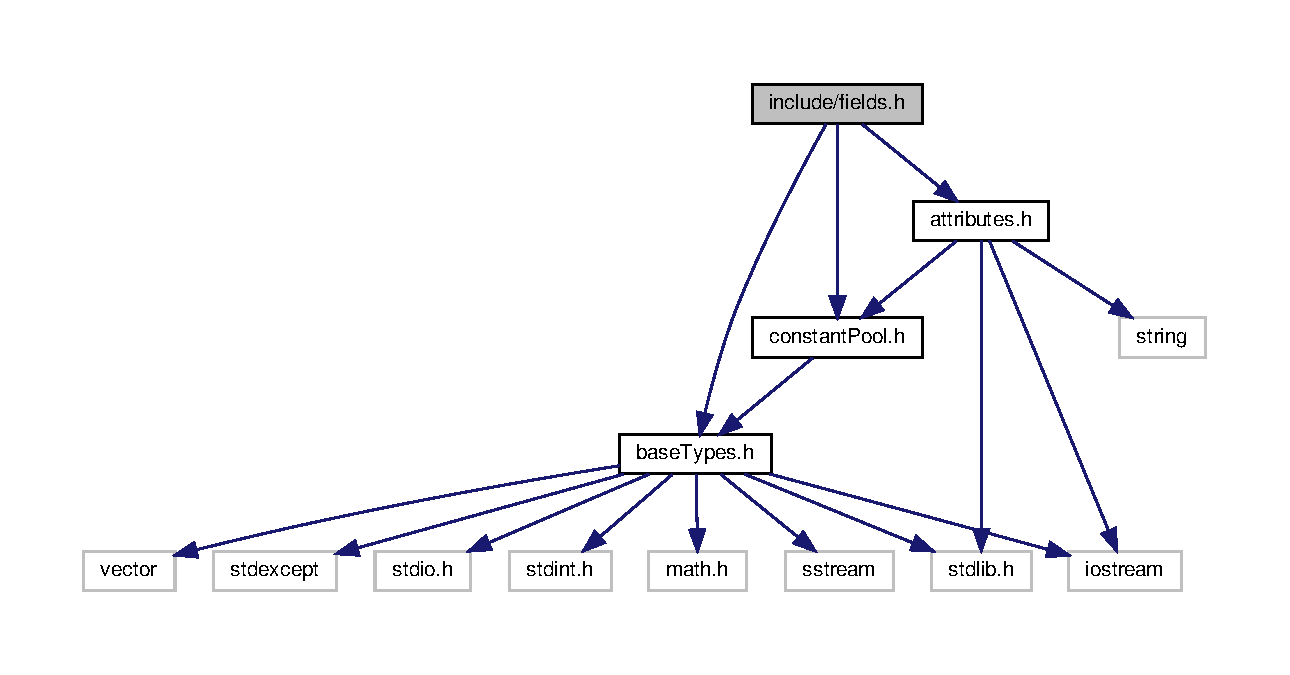
\includegraphics[width=350pt]{fields_8h__incl}
\end{center}
\end{figure}
Este grafo mostra quais são os ficheiros que incluem directamente ou indirectamente este ficheiro\+:
\nopagebreak
\begin{figure}[H]
\begin{center}
\leavevmode
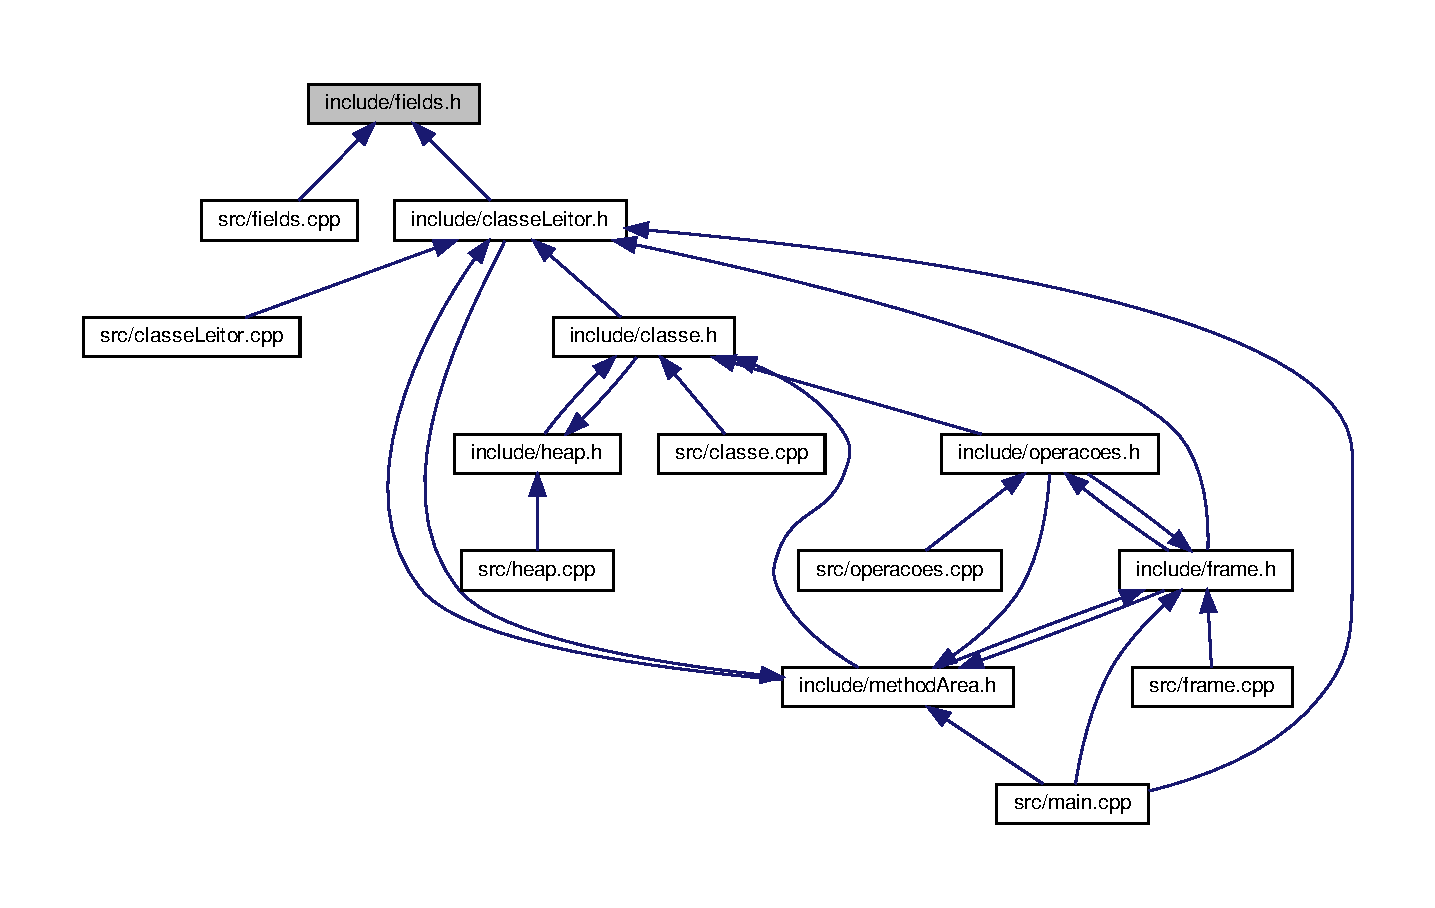
\includegraphics[width=350pt]{fields_8h__dep__incl}
\end{center}
\end{figure}
\subsection*{Estruturas de Dados}
\begin{DoxyCompactItemize}
\item 
struct \hyperlink{structfield__info}{field\+\_\+info}
\begin{DoxyCompactList}\small\item\em Struct de armazenamento. \end{DoxyCompactList}\end{DoxyCompactItemize}
\subsection*{Funções}
\begin{DoxyCompactItemize}
\item 
string \hyperlink{fields_8h_a8b0a792b5f197e376c9f92ec12fda1d8}{get\+Field\+Flags} (unsigned short flags)
\begin{DoxyCompactList}\small\item\em Função para mostrar as flags dos campos. \end{DoxyCompactList}\item 
\hyperlink{structfield__info}{field\+\_\+info} \hyperlink{fields_8h_a95a676570bdecf7ee0595e28472f6b4c}{read\+Field} (F\+I\+LE $\ast$fp, \hyperlink{structcp__info}{cp\+\_\+info} $\ast$cp)
\begin{DoxyCompactList}\small\item\em Função que lê um campo. \end{DoxyCompactList}\item 
\hyperlink{structfield__info}{field\+\_\+info} $\ast$ \hyperlink{fields_8h_a1eb34923f335ccdf5bed84dec284d907}{read\+Fields} (F\+I\+LE $\ast$fp, int length, \hyperlink{structcp__info}{cp\+\_\+info} $\ast$cp)
\begin{DoxyCompactList}\small\item\em Função que aloca \hyperlink{structfield__info}{field\+\_\+info} espaço e chama read\+Field \char`\"{}lenght\char`\"{} vezes. \end{DoxyCompactList}\item 
\mbox{\Hypertarget{fields_8h_a3bba8cdcee17336a5484fb8a9d4bcd92}\label{fields_8h_a3bba8cdcee17336a5484fb8a9d4bcd92}} 
void {\bfseries print\+Field} (\hyperlink{structfield__info}{field\+\_\+info} f, \hyperlink{structcp__info}{cp\+\_\+info} $\ast$cp, int index)
\item 
void \hyperlink{fields_8h_a51b92b23bc1d716b7497c2574577c563}{print\+Fields} (\hyperlink{structfield__info}{field\+\_\+info} $\ast$f, \hyperlink{structcp__info}{cp\+\_\+info} $\ast$cp, int length)
\begin{DoxyCompactList}\small\item\em Fuunção que chama print\+Field o número de vezes determinado por \char`\"{}length\char`\"{}. \end{DoxyCompactList}\end{DoxyCompactItemize}


\subsection{Descrição detalhada}
Classe field. 

Field used at archives with .class format 

\subsection{Documentação das funções}
\mbox{\Hypertarget{fields_8h_a8b0a792b5f197e376c9f92ec12fda1d8}\label{fields_8h_a8b0a792b5f197e376c9f92ec12fda1d8}} 
\index{fields.\+h@{fields.\+h}!get\+Field\+Flags@{get\+Field\+Flags}}
\index{get\+Field\+Flags@{get\+Field\+Flags}!fields.\+h@{fields.\+h}}
\subsubsection{\texorpdfstring{get\+Field\+Flags()}{getFieldFlags()}}
{\footnotesize\ttfamily string get\+Field\+Flags (\begin{DoxyParamCaption}\item[{unsigned short}]{flags }\end{DoxyParamCaption})}



Função para mostrar as flags dos campos. 


\begin{DoxyParams}{Parâmetros}
{\em flags} & Flags em haxadecimal que serão convertidas para string. \\
\hline
\end{DoxyParams}
\mbox{\Hypertarget{fields_8h_a51b92b23bc1d716b7497c2574577c563}\label{fields_8h_a51b92b23bc1d716b7497c2574577c563}} 
\index{fields.\+h@{fields.\+h}!print\+Fields@{print\+Fields}}
\index{print\+Fields@{print\+Fields}!fields.\+h@{fields.\+h}}
\subsubsection{\texorpdfstring{print\+Fields()}{printFields()}}
{\footnotesize\ttfamily void print\+Fields (\begin{DoxyParamCaption}\item[{\hyperlink{structfield__info}{field\+\_\+info} $\ast$}]{f,  }\item[{\hyperlink{structcp__info}{cp\+\_\+info} $\ast$}]{cp,  }\item[{int}]{length }\end{DoxyParamCaption})}



Fuunção que chama print\+Field o número de vezes determinado por \char`\"{}length\char`\"{}. 


\begin{DoxyParams}{Parâmetros}
{\em f} & Struct que contém informação dos campos. \\
\hline
{\em cp} & Ponteiro para pool de constantes. \\
\hline
{\em length} & Define o número de chamadas à print\+Field. \\
\hline
\end{DoxyParams}
\mbox{\Hypertarget{fields_8h_a95a676570bdecf7ee0595e28472f6b4c}\label{fields_8h_a95a676570bdecf7ee0595e28472f6b4c}} 
\index{fields.\+h@{fields.\+h}!read\+Field@{read\+Field}}
\index{read\+Field@{read\+Field}!fields.\+h@{fields.\+h}}
\subsubsection{\texorpdfstring{read\+Field()}{readField()}}
{\footnotesize\ttfamily \hyperlink{structfield__info}{field\+\_\+info} read\+Field (\begin{DoxyParamCaption}\item[{F\+I\+LE $\ast$}]{fp,  }\item[{\hyperlink{structcp__info}{cp\+\_\+info} $\ast$}]{cp }\end{DoxyParamCaption})}



Função que lê um campo. 


\begin{DoxyParams}{Parâmetros}
{\em fp} & Ponteiro para arquivo .class. \\
\hline
{\em cp} & Ponteiro para pool de constantes. \\
\hline
\end{DoxyParams}
\mbox{\Hypertarget{fields_8h_a1eb34923f335ccdf5bed84dec284d907}\label{fields_8h_a1eb34923f335ccdf5bed84dec284d907}} 
\index{fields.\+h@{fields.\+h}!read\+Fields@{read\+Fields}}
\index{read\+Fields@{read\+Fields}!fields.\+h@{fields.\+h}}
\subsubsection{\texorpdfstring{read\+Fields()}{readFields()}}
{\footnotesize\ttfamily \hyperlink{structfield__info}{field\+\_\+info}$\ast$ read\+Fields (\begin{DoxyParamCaption}\item[{F\+I\+LE $\ast$}]{fp,  }\item[{int}]{length,  }\item[{\hyperlink{structcp__info}{cp\+\_\+info} $\ast$}]{cp }\end{DoxyParamCaption})}



Função que aloca \hyperlink{structfield__info}{field\+\_\+info} espaço e chama read\+Field \char`\"{}lenght\char`\"{} vezes. 


\begin{DoxyParams}{Parâmetros}
{\em fp} & Ponteiro para arquivo .class. \\
\hline
{\em cp} & Ponteiro para pool de constantes. \\
\hline
{\em length} & Define o número de chamadas à read\+Field. \\
\hline
\end{DoxyParams}

\hypertarget{frame_8h}{}\section{Referência ao ficheiro include/frame.h}
\label{frame_8h}\index{include/frame.\+h@{include/frame.\+h}}


Contém tudo necessário para a execução de um método.  


{\ttfamily \#include \char`\"{}classe\+Leitor.\+h\char`\"{}}\newline
{\ttfamily \#include \char`\"{}pilha\+Operandos.\+h\char`\"{}}\newline
{\ttfamily \#include \char`\"{}local\+Variables.\+h\char`\"{}}\newline
{\ttfamily \#include \char`\"{}base\+Types.\+h\char`\"{}}\newline
{\ttfamily \#include \char`\"{}operacoes.\+h\char`\"{}}\newline
{\ttfamily \#include \char`\"{}attributes.\+h\char`\"{}}\newline
{\ttfamily \#include \char`\"{}method\+Area.\+h\char`\"{}}\newline
Diagrama de dependências de inclusão para frame.\+h\+:
\nopagebreak
\begin{figure}[H]
\begin{center}
\leavevmode
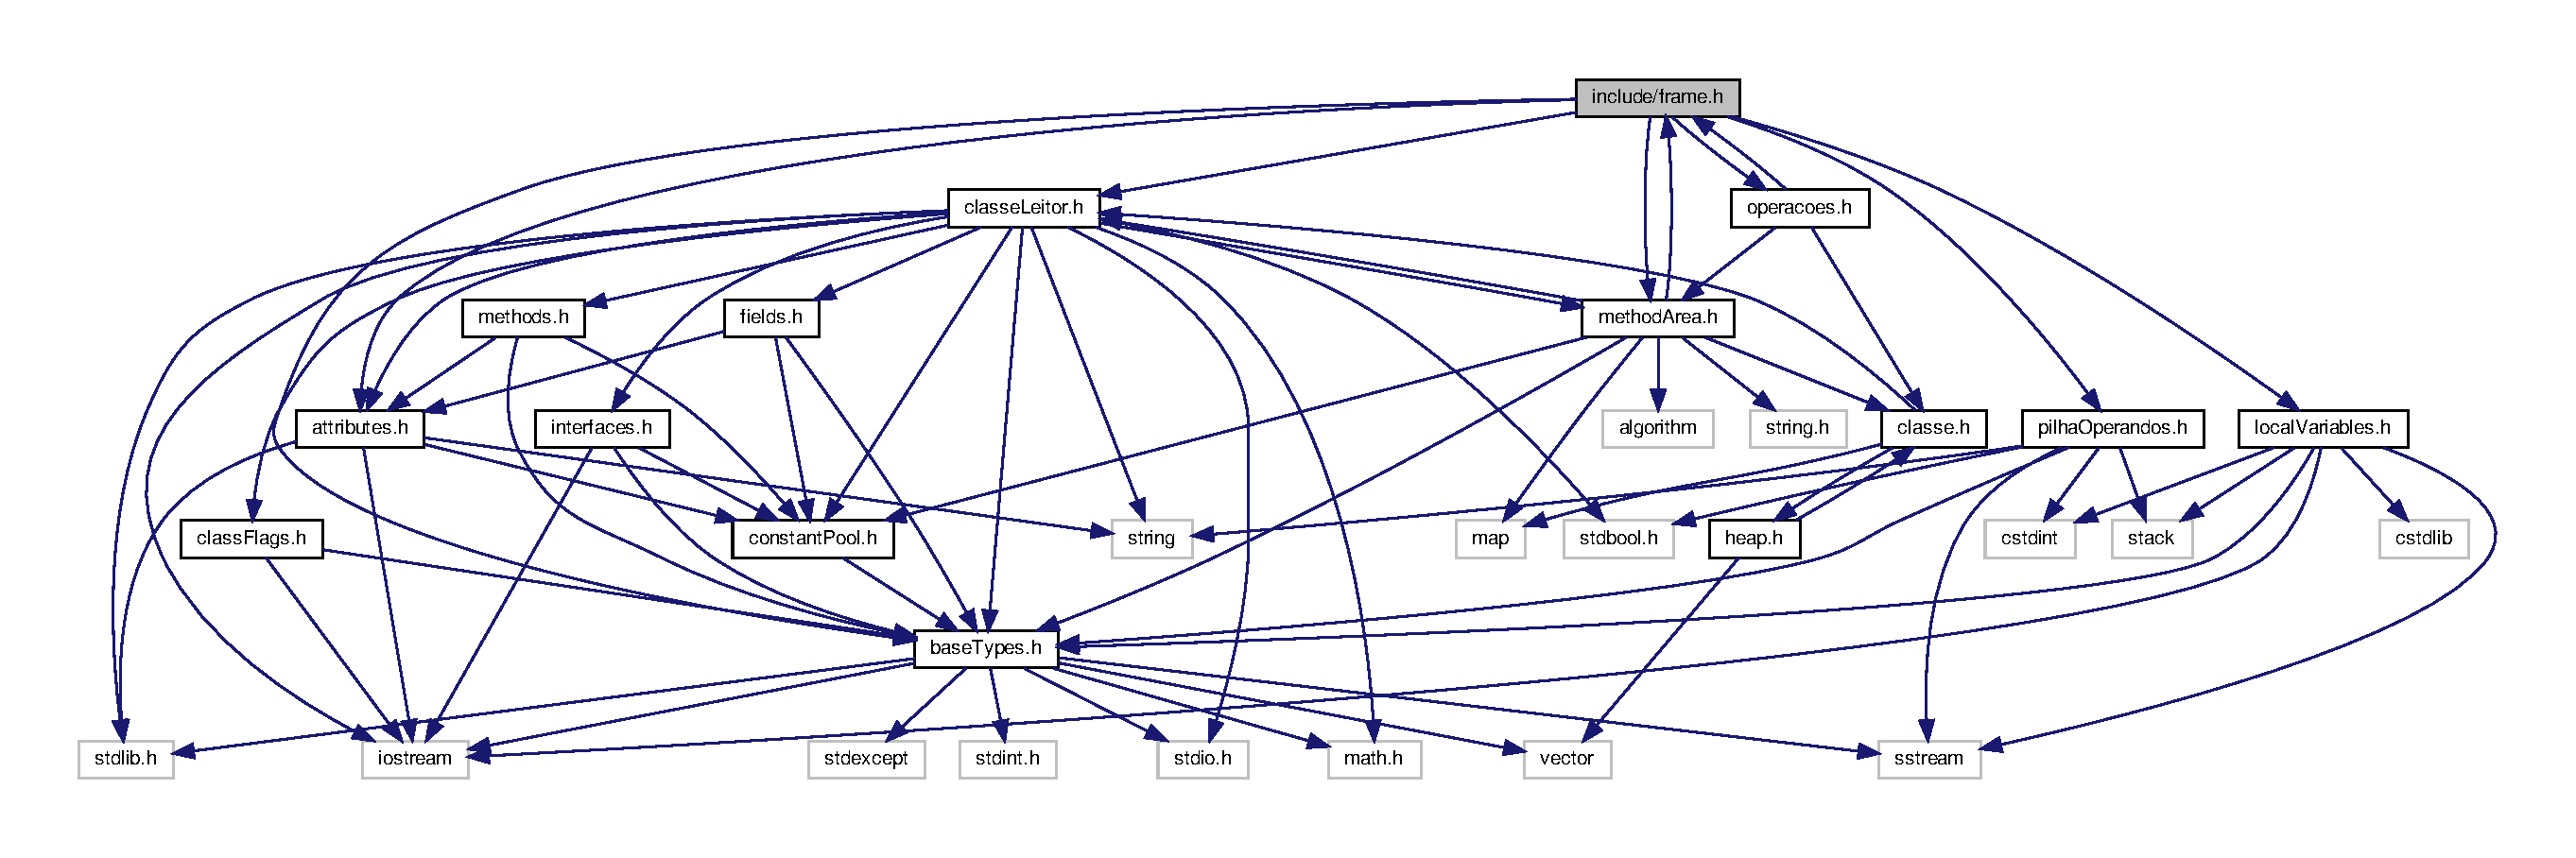
\includegraphics[width=350pt]{frame_8h__incl}
\end{center}
\end{figure}
Este grafo mostra quais são os ficheiros que incluem directamente ou indirectamente este ficheiro\+:
\nopagebreak
\begin{figure}[H]
\begin{center}
\leavevmode
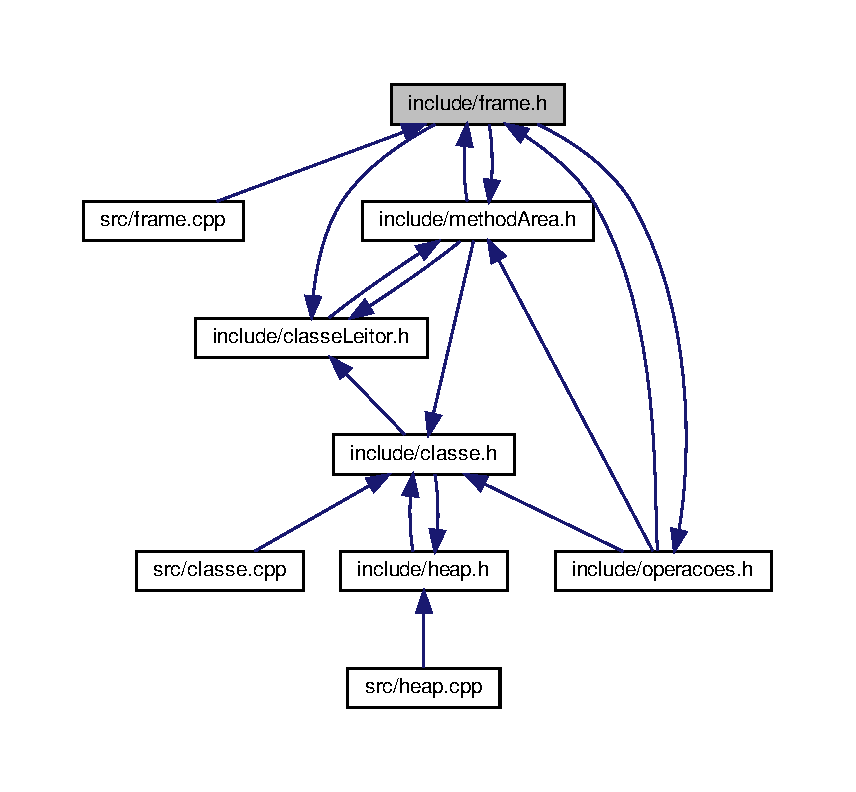
\includegraphics[width=350pt]{frame_8h__dep__incl}
\end{center}
\end{figure}
\subsection*{Estruturas de Dados}
\begin{DoxyCompactItemize}
\item 
struct \hyperlink{structframe__s}{frame\+\_\+s}
\begin{DoxyCompactList}\small\item\em Estrutura de armazenamento. \end{DoxyCompactList}\item 
class \hyperlink{classFrameStack}{Frame\+Stack}
\begin{DoxyCompactList}\small\item\em Classe de pilha de frames. \end{DoxyCompactList}\end{DoxyCompactItemize}
\subsection*{Definições de tipos}
\begin{DoxyCompactItemize}
\item 
\mbox{\Hypertarget{frame_8h_aeaf3b41036669d78da398fbc7877886d}\label{frame_8h_aeaf3b41036669d78da398fbc7877886d}} 
typedef struct \hyperlink{structframe__s}{frame\+\_\+s} {\bfseries frame}
\end{DoxyCompactItemize}


\subsection{Descrição detalhada}
Contém tudo necessário para a execução de um método. 


\hypertarget{heap_8h}{}\section{Referência ao ficheiro include/heap.h}
\label{heap_8h}\index{include/heap.\+h@{include/heap.\+h}}


Definição do \hyperlink{classHeap}{Heap}.  


{\ttfamily \#include \char`\"{}classe.\+h\char`\"{}}\newline
{\ttfamily \#include $<$vector$>$}\newline
Diagrama de dependências de inclusão para heap.\+h\+:
\nopagebreak
\begin{figure}[H]
\begin{center}
\leavevmode
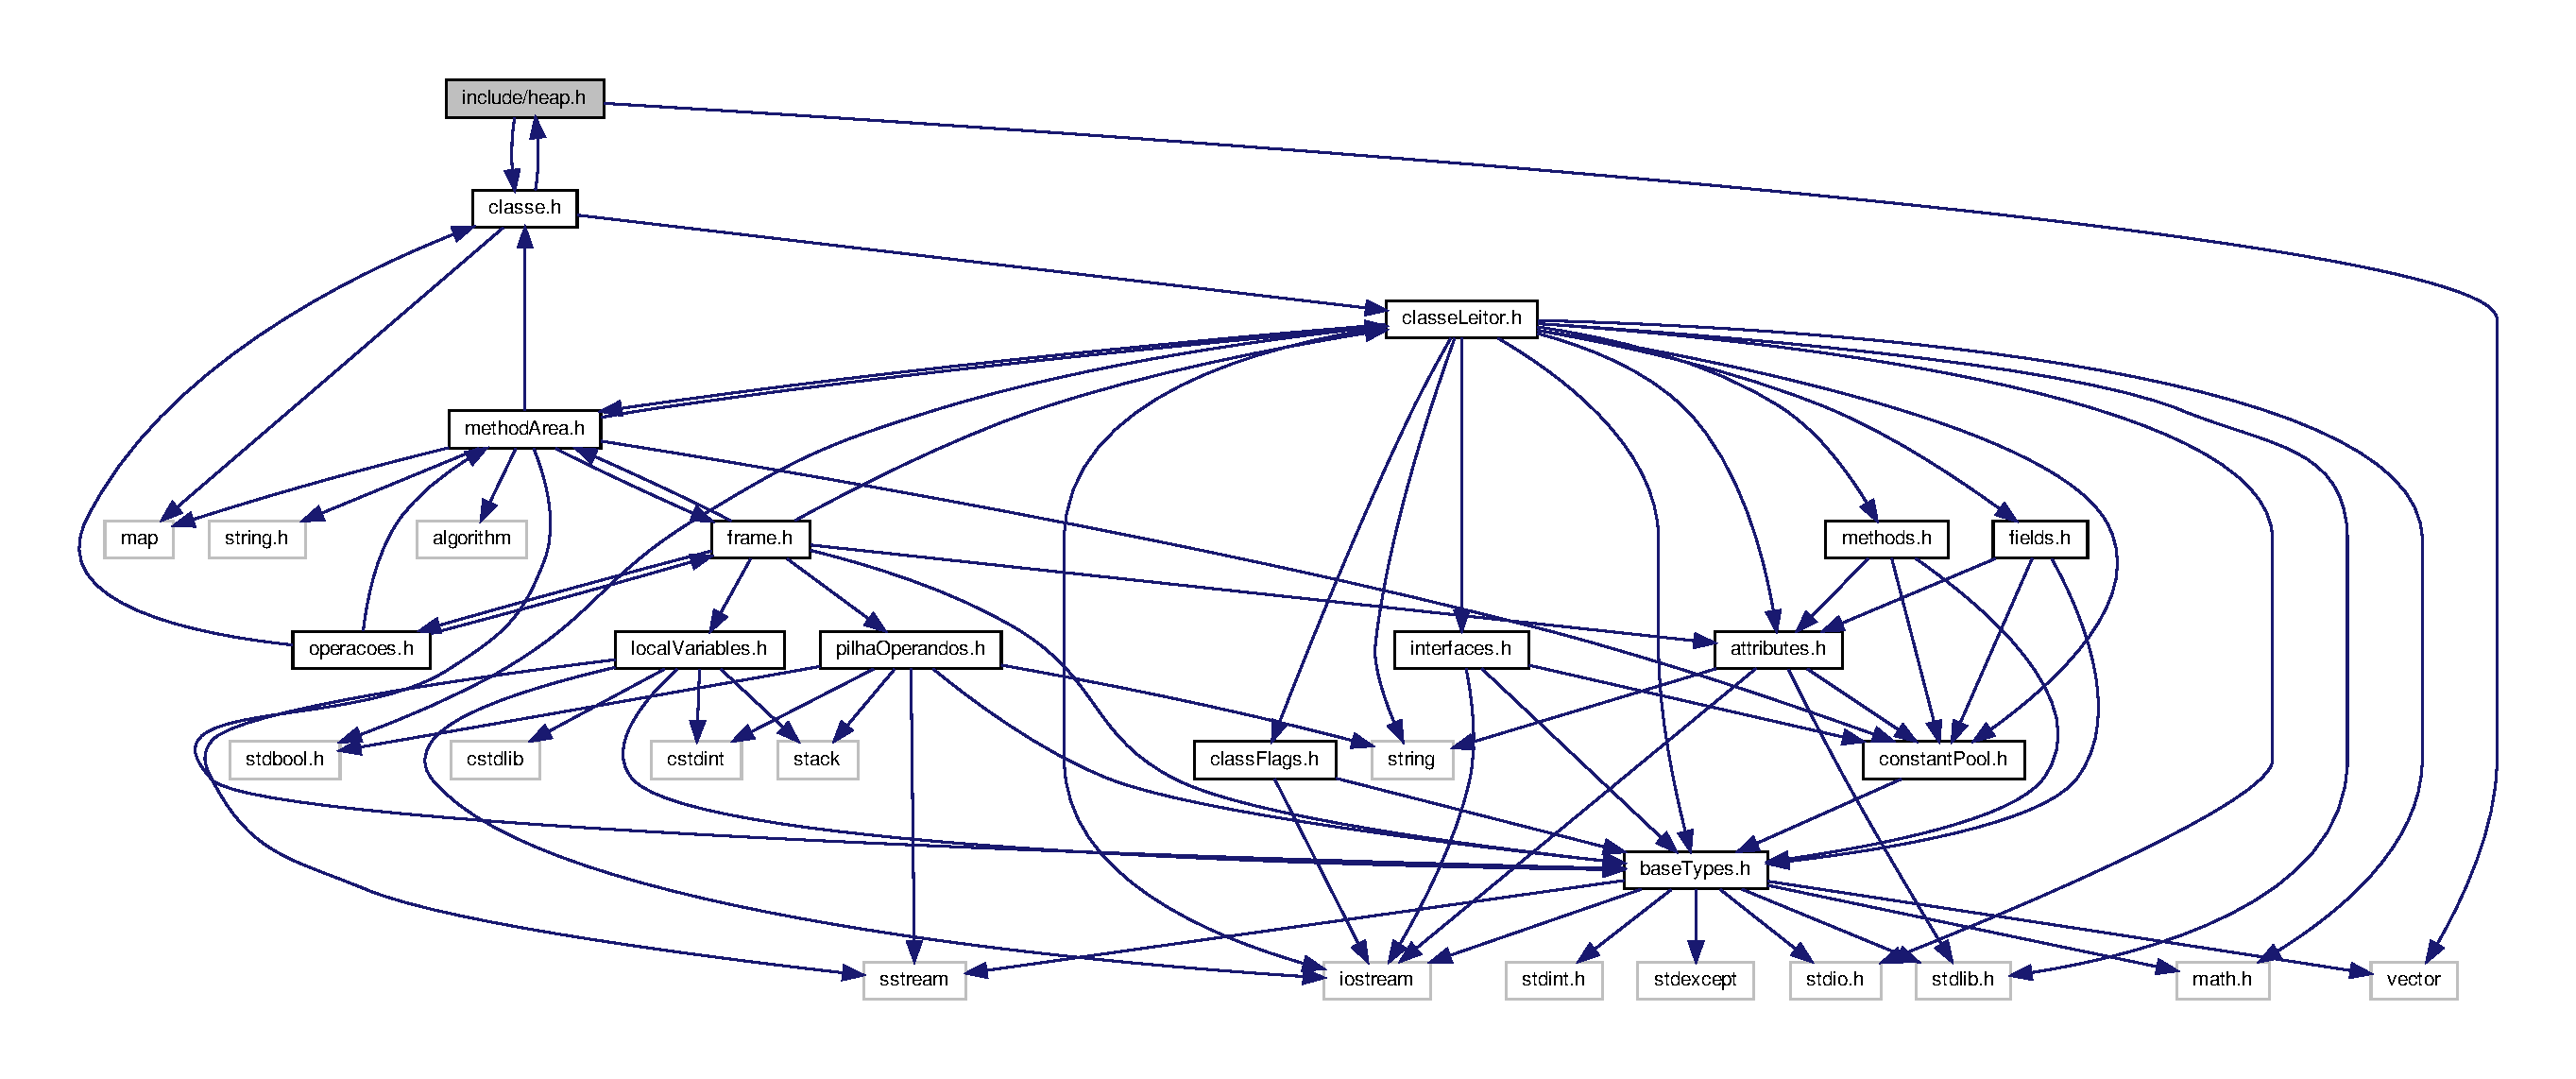
\includegraphics[width=350pt]{heap_8h__incl}
\end{center}
\end{figure}
Este grafo mostra quais são os ficheiros que incluem directamente ou indirectamente este ficheiro\+:
\nopagebreak
\begin{figure}[H]
\begin{center}
\leavevmode
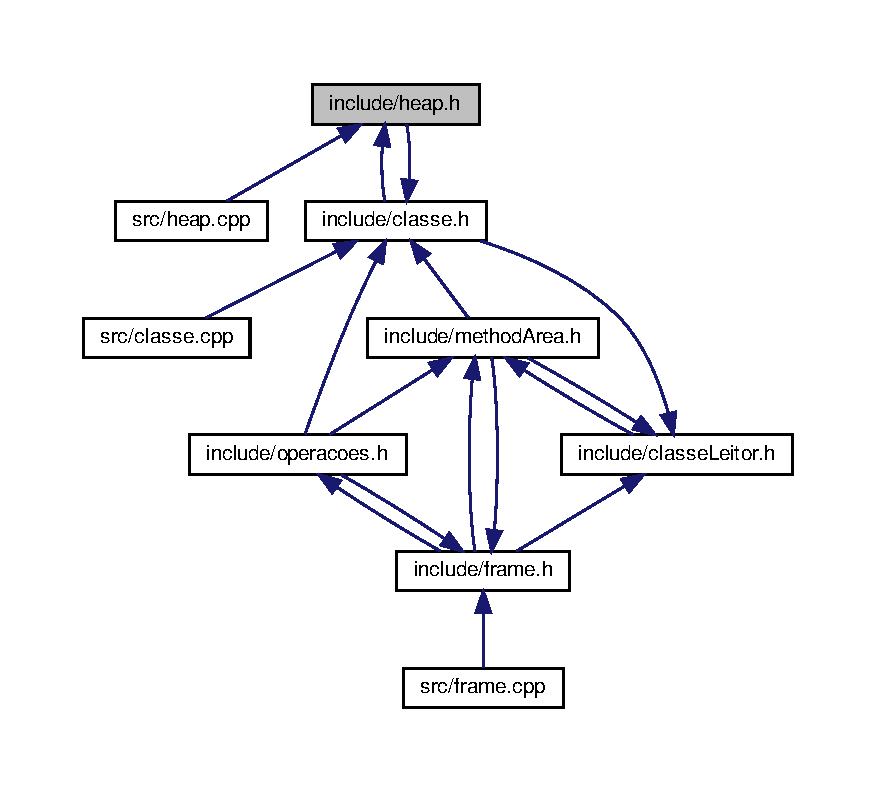
\includegraphics[width=350pt]{heap_8h__dep__incl}
\end{center}
\end{figure}
\subsection*{Estruturas de Dados}
\begin{DoxyCompactItemize}
\item 
class \hyperlink{classHeap}{Heap}
\begin{DoxyCompactList}\small\item\em Classe do heap. \end{DoxyCompactList}\end{DoxyCompactItemize}


\subsection{Descrição detalhada}
Definição do \hyperlink{classHeap}{Heap}. 

Gerencia a execução do heap. 
\hypertarget{interfaces_8h}{}\section{Referência ao ficheiro include/interfaces.h}
\label{interfaces_8h}\index{include/interfaces.\+h@{include/interfaces.\+h}}


Interfaces.  


{\ttfamily \#include $<$iostream$>$}\newline
{\ttfamily \#include \char`\"{}constant\+Pool.\+h\char`\"{}}\newline
{\ttfamily \#include \char`\"{}base\+Types.\+h\char`\"{}}\newline
Diagrama de dependências de inclusão para interfaces.\+h\+:\nopagebreak
\begin{figure}[H]
\begin{center}
\leavevmode
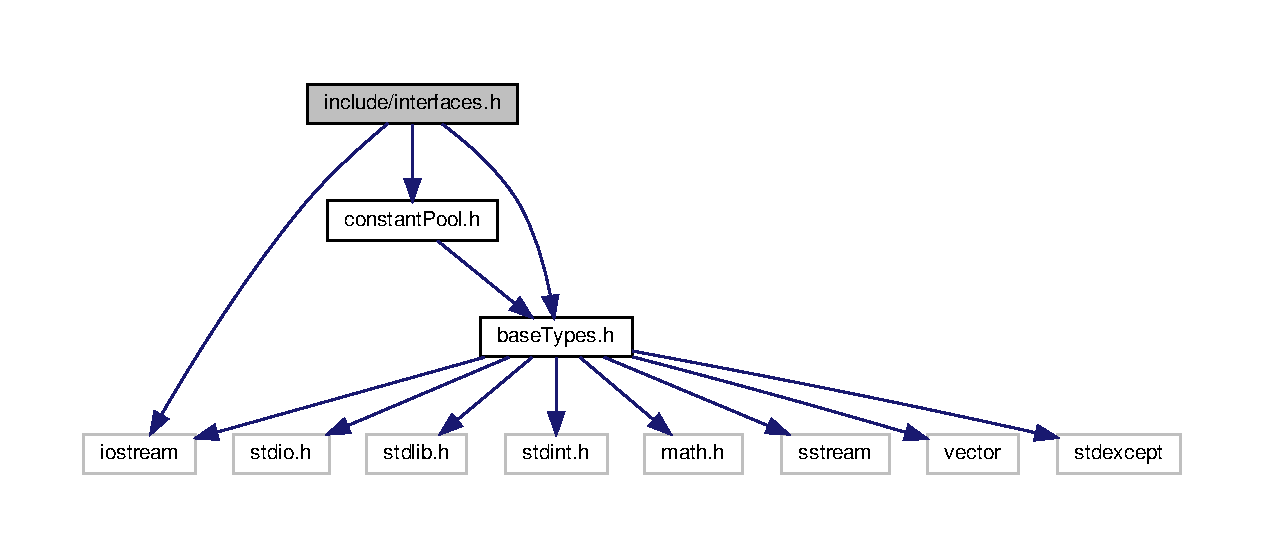
\includegraphics[width=350pt]{interfaces_8h__incl}
\end{center}
\end{figure}
Este grafo mostra quais são os ficheiros que incluem directamente ou indirectamente este ficheiro\+:\nopagebreak
\begin{figure}[H]
\begin{center}
\leavevmode
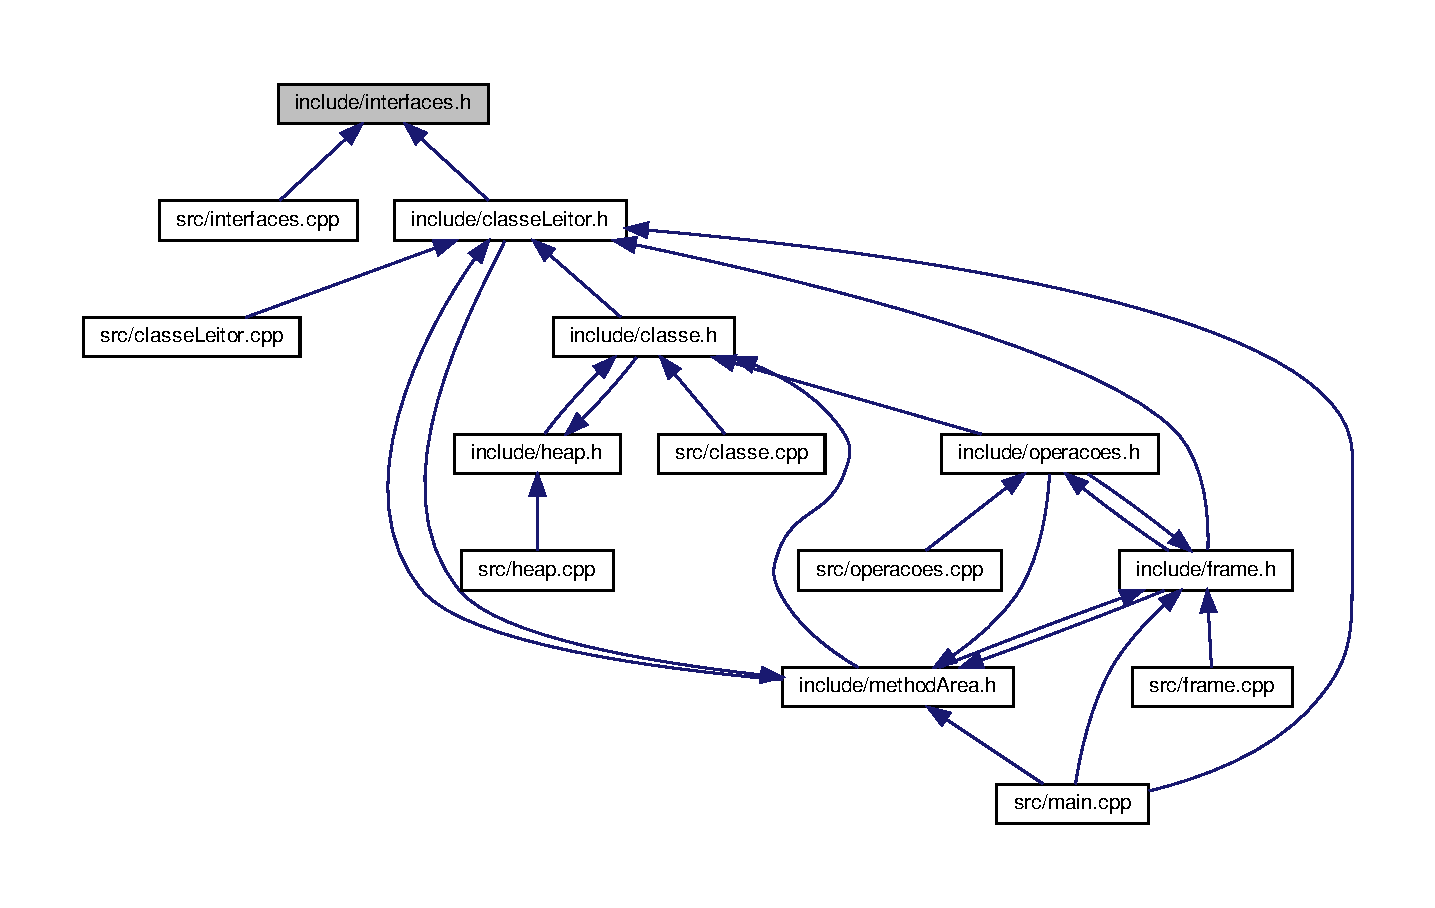
\includegraphics[width=350pt]{interfaces_8h__dep__incl}
\end{center}
\end{figure}
\subsection*{Funções}
\begin{DoxyCompactItemize}
\item 
unsigned short $\ast$ \hyperlink{interfaces_8h_ae922cb6cdd2af5a0da3f039d03b230c7}{read\+Interfaces} (F\+I\+LE $\ast$fp, int length)
\begin{DoxyCompactList}\small\item\em Carrega as interfaces na mem�ria a partir do arquivo class. \end{DoxyCompactList}\item 
void \hyperlink{interfaces_8h_a6ec7de60877b4db37aecdb7cf818c863}{print\+Interfaces} (unsigned short $\ast$interfaces, \hyperlink{structcp__info}{cp\+\_\+info} $\ast$cp, int length)
\begin{DoxyCompactList}\small\item\em Mostra todas as interfaces do arquivo. \end{DoxyCompactList}\item 
void \hyperlink{interfaces_8h_aac94a426e29da5419540d2e54e96f7fa}{print\+Interface} (unsigned short interface, \hyperlink{structcp__info}{cp\+\_\+info} $\ast$cp)
\begin{DoxyCompactList}\small\item\em Mostra informa��es de uma interface espec�fica. \end{DoxyCompactList}\item 
void \hyperlink{interfaces_8h_aecd49471b21a9c29d2f88f757b1734ad}{print\+Interface} (unsigned short interface, \hyperlink{structcp__info}{cp\+\_\+info} $\ast$cp, int index)
\begin{DoxyCompactList}\small\item\em Mostra informa��o de uma interface espec�fica com o �ndice da interface. \end{DoxyCompactList}\end{DoxyCompactItemize}


\subsection{Descrição detalhada}
Interfaces. 

Manipula as informa��es de interface do .class 

\subsection{Documentação das funções}
\mbox{\Hypertarget{interfaces_8h_aac94a426e29da5419540d2e54e96f7fa}\label{interfaces_8h_aac94a426e29da5419540d2e54e96f7fa}} 
\index{interfaces.\+h@{interfaces.\+h}!print\+Interface@{print\+Interface}}
\index{print\+Interface@{print\+Interface}!interfaces.\+h@{interfaces.\+h}}
\subsubsection{\texorpdfstring{print\+Interface()}{printInterface()}\hspace{0.1cm}{\footnotesize\ttfamily [1/2]}}
{\footnotesize\ttfamily print\+Interface (\begin{DoxyParamCaption}\item[{unsigned short}]{interface,  }\item[{\hyperlink{structcp__info}{cp\+\_\+info} $\ast$}]{cp }\end{DoxyParamCaption})}



Mostra informa��es de uma interface espec�fica. 


\begin{DoxyParams}{Parâmetros}
{\em interface} & Indice do constantpool. \\
\hline
{\em cp} & Ponteiro para a constantpool. \\
\hline
\end{DoxyParams}
\mbox{\Hypertarget{interfaces_8h_aecd49471b21a9c29d2f88f757b1734ad}\label{interfaces_8h_aecd49471b21a9c29d2f88f757b1734ad}} 
\index{interfaces.\+h@{interfaces.\+h}!print\+Interface@{print\+Interface}}
\index{print\+Interface@{print\+Interface}!interfaces.\+h@{interfaces.\+h}}
\subsubsection{\texorpdfstring{print\+Interface()}{printInterface()}\hspace{0.1cm}{\footnotesize\ttfamily [2/2]}}
{\footnotesize\ttfamily void print\+Interface (\begin{DoxyParamCaption}\item[{unsigned short}]{interface,  }\item[{\hyperlink{structcp__info}{cp\+\_\+info} $\ast$}]{cp,  }\item[{int}]{index }\end{DoxyParamCaption})}



Mostra informa��o de uma interface espec�fica com o �ndice da interface. 


\begin{DoxyParams}{Parâmetros}
{\em interface} & Indice do constantpool. \\
\hline
{\em cp} & Ponteiro para o constantpool. \\
\hline
{\em index} & Indice da interface espec�fica. \\
\hline
\end{DoxyParams}
\mbox{\Hypertarget{interfaces_8h_a6ec7de60877b4db37aecdb7cf818c863}\label{interfaces_8h_a6ec7de60877b4db37aecdb7cf818c863}} 
\index{interfaces.\+h@{interfaces.\+h}!print\+Interfaces@{print\+Interfaces}}
\index{print\+Interfaces@{print\+Interfaces}!interfaces.\+h@{interfaces.\+h}}
\subsubsection{\texorpdfstring{print\+Interfaces()}{printInterfaces()}}
{\footnotesize\ttfamily void print\+Interfaces (\begin{DoxyParamCaption}\item[{unsigned short $\ast$}]{interfaces,  }\item[{\hyperlink{structcp__info}{cp\+\_\+info} $\ast$}]{cp,  }\item[{int}]{length }\end{DoxyParamCaption})}



Mostra todas as interfaces do arquivo. 


\begin{DoxyParams}{Parâmetros}
{\em interfaces} & Array de interfaces. \\
\hline
{\em cp} & Ponteiro para a constantpool. \\
\hline
{\em length} & N�mero de interfaces. \\
\hline
\end{DoxyParams}
\mbox{\Hypertarget{interfaces_8h_ae922cb6cdd2af5a0da3f039d03b230c7}\label{interfaces_8h_ae922cb6cdd2af5a0da3f039d03b230c7}} 
\index{interfaces.\+h@{interfaces.\+h}!read\+Interfaces@{read\+Interfaces}}
\index{read\+Interfaces@{read\+Interfaces}!interfaces.\+h@{interfaces.\+h}}
\subsubsection{\texorpdfstring{read\+Interfaces()}{readInterfaces()}}
{\footnotesize\ttfamily unsigned short$\ast$ read\+Interfaces (\begin{DoxyParamCaption}\item[{F\+I\+LE $\ast$}]{fp,  }\item[{int}]{length }\end{DoxyParamCaption})}



Carrega as interfaces na mem�ria a partir do arquivo class. 


\begin{DoxyParams}{Parâmetros}
{\em flags} & Flags em haxadecimal que ser�o convertidas para string. \\
\hline
{\em fp} & Ponteiro para o arquivo class. \\
\hline
{\em length} & Numero de interfaces a serem lidas. \\
\hline
\end{DoxyParams}

\hypertarget{localVariables_8h}{}\section{Referência ao ficheiro include/local\+Variables.h}
\label{localVariables_8h}\index{include/local\+Variables.\+h@{include/local\+Variables.\+h}}


Local Variables.  


{\ttfamily \#include $<$cstdint$>$}\newline
{\ttfamily \#include $<$stack$>$}\newline
{\ttfamily \#include $<$iostream$>$}\newline
{\ttfamily \#include $<$sstream$>$}\newline
{\ttfamily \#include $<$cstdlib$>$}\newline
{\ttfamily \#include \char`\"{}base\+Types.\+h\char`\"{}}\newline
Diagrama de dependências de inclusão para local\+Variables.\+h\+:\nopagebreak
\begin{figure}[H]
\begin{center}
\leavevmode
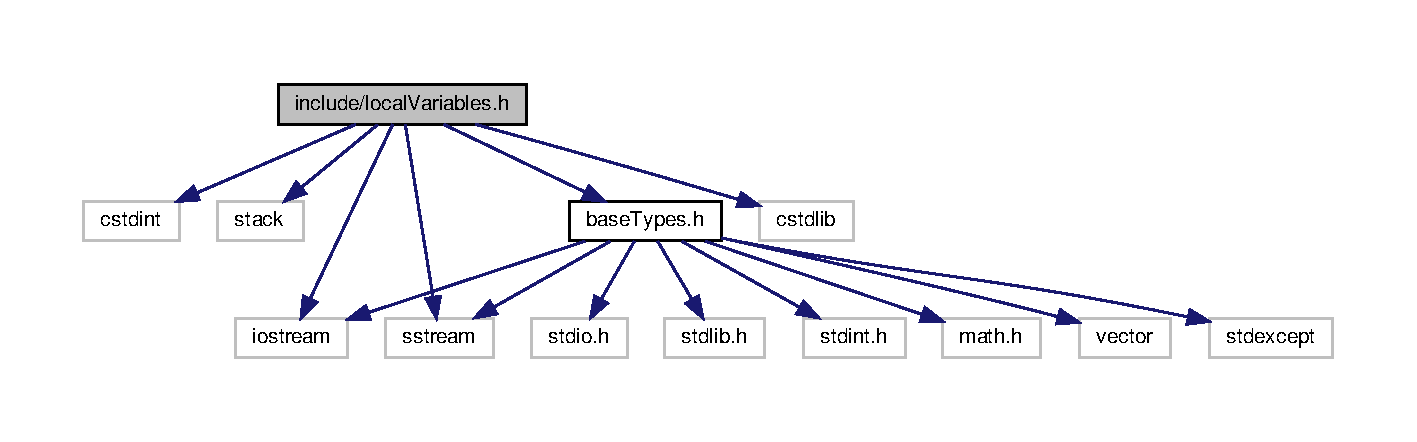
\includegraphics[width=350pt]{localVariables_8h__incl}
\end{center}
\end{figure}
Este grafo mostra quais são os ficheiros que incluem directamente ou indirectamente este ficheiro\+:
\nopagebreak
\begin{figure}[H]
\begin{center}
\leavevmode
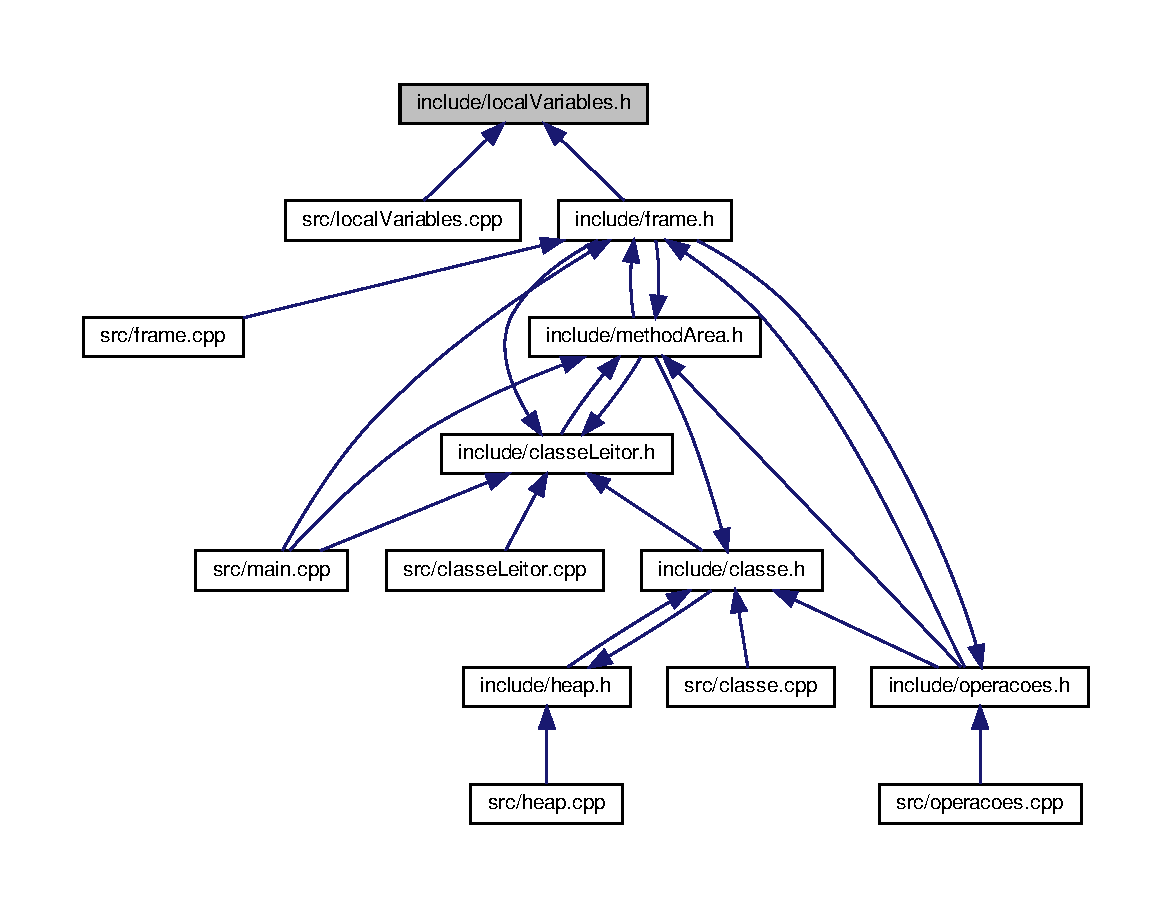
\includegraphics[width=350pt]{localVariables_8h__dep__incl}
\end{center}
\end{figure}
\subsection*{Estruturas de Dados}
\begin{DoxyCompactItemize}
\item 
class \hyperlink{classLocalVariables}{Local\+Variables}
\begin{DoxyCompactList}\small\item\em Local variables Class. \end{DoxyCompactList}\end{DoxyCompactItemize}
\subsection*{Macros}
\begin{DoxyCompactItemize}
\item 
\mbox{\Hypertarget{localVariables_8h_a9d2a7c69bd3fabc41e1ee87df2f283b3}\label{localVariables_8h_a9d2a7c69bd3fabc41e1ee87df2f283b3}} 
\#define {\bfseries B\+I\+TS}~(sizeof(int$\ast$) == 8)
\item 
\mbox{\Hypertarget{localVariables_8h_adf770fe2eec438e3758ffe905dbae208}\label{localVariables_8h_adf770fe2eec438e3758ffe905dbae208}} 
\#define {\bfseries I\+N\+V\+A\+L\+ID}~99
\item 
\mbox{\Hypertarget{localVariables_8h_a0623cf1b3dda05505734b67f550c53cb}\label{localVariables_8h_a0623cf1b3dda05505734b67f550c53cb}} 
\#define {\bfseries T\+Y\+P\+E\+\_\+\+N\+O\+T\+\_\+\+S\+ET}~0
\item 
\mbox{\Hypertarget{localVariables_8h_a56e5f9a95536838408fcca8f22d541b4}\label{localVariables_8h_a56e5f9a95536838408fcca8f22d541b4}} 
\#define {\bfseries T\+Y\+P\+E\+\_\+\+I\+NT}~1
\item 
\mbox{\Hypertarget{localVariables_8h_a105c7addfad52601f4d079673eae7982}\label{localVariables_8h_a105c7addfad52601f4d079673eae7982}} 
\#define {\bfseries T\+Y\+P\+E\+\_\+\+F\+L\+O\+AT}~2
\item 
\mbox{\Hypertarget{localVariables_8h_a64b164f200989fc609ff40c0e1aa2518}\label{localVariables_8h_a64b164f200989fc609ff40c0e1aa2518}} 
\#define {\bfseries T\+Y\+P\+E\+\_\+\+L\+O\+NG}~3
\item 
\mbox{\Hypertarget{localVariables_8h_ac87fa650bc0dcd101b39e15ecdb57477}\label{localVariables_8h_ac87fa650bc0dcd101b39e15ecdb57477}} 
\#define {\bfseries T\+Y\+P\+E\+\_\+\+D\+O\+U\+B\+LE}~4
\item 
\mbox{\Hypertarget{localVariables_8h_a375775d23dbf60915db33f1add80c006}\label{localVariables_8h_a375775d23dbf60915db33f1add80c006}} 
\#define {\bfseries T\+Y\+P\+E\+\_\+\+B\+O\+OL}~5
\item 
\mbox{\Hypertarget{localVariables_8h_aa1e9e57b2fa5fdc501d79de85b69c986}\label{localVariables_8h_aa1e9e57b2fa5fdc501d79de85b69c986}} 
\#define {\bfseries T\+Y\+P\+E\+\_\+\+R\+E\+F\+E\+R\+E\+N\+CE}~6
\end{DoxyCompactItemize}


\subsection{Descrição detalhada}
Local Variables. 

Stores local variables to current method 
\hypertarget{pilhaOperandos_8h}{}\section{Referência ao ficheiro include/pilha\+Operandos.h}
\label{pilhaOperandos_8h}\index{include/pilha\+Operandos.\+h@{include/pilha\+Operandos.\+h}}


Pilha de operandos.  


{\ttfamily \#include $<$stack$>$}\newline
{\ttfamily \#include $<$cstdint$>$}\newline
{\ttfamily \#include $<$string$>$}\newline
{\ttfamily \#include $<$sstream$>$}\newline
{\ttfamily \#include $<$stdbool.\+h$>$}\newline
{\ttfamily \#include \char`\"{}base\+Types.\+h\char`\"{}}\newline
Diagrama de dependências de inclusão para pilha\+Operandos.\+h\+:\nopagebreak
\begin{figure}[H]
\begin{center}
\leavevmode
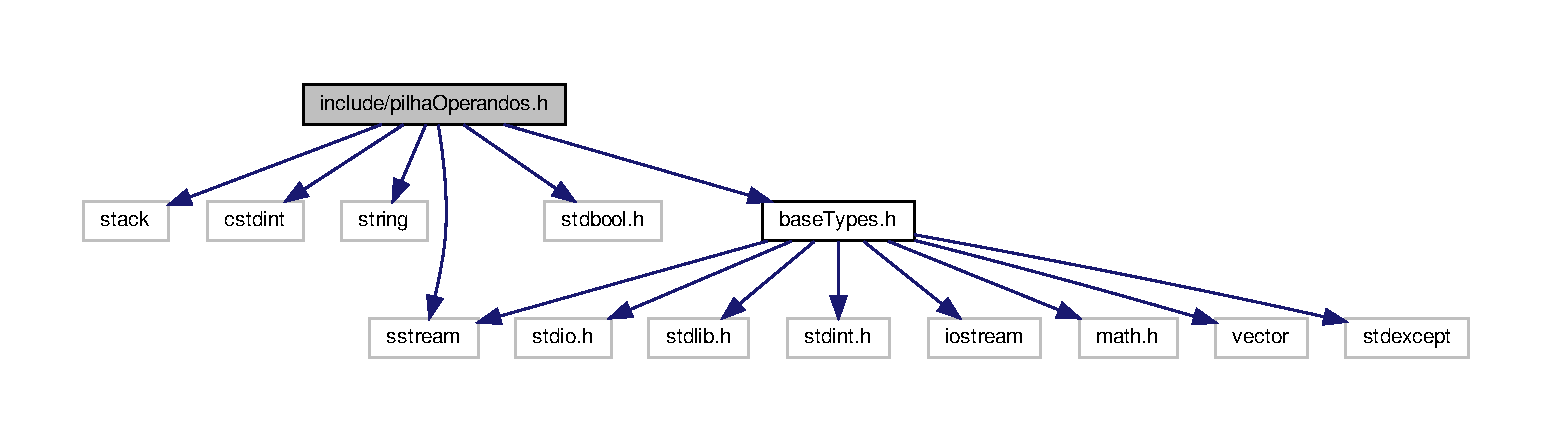
\includegraphics[width=350pt]{pilhaOperandos_8h__incl}
\end{center}
\end{figure}
Este grafo mostra quais são os ficheiros que incluem directamente ou indirectamente este ficheiro\+:
\nopagebreak
\begin{figure}[H]
\begin{center}
\leavevmode
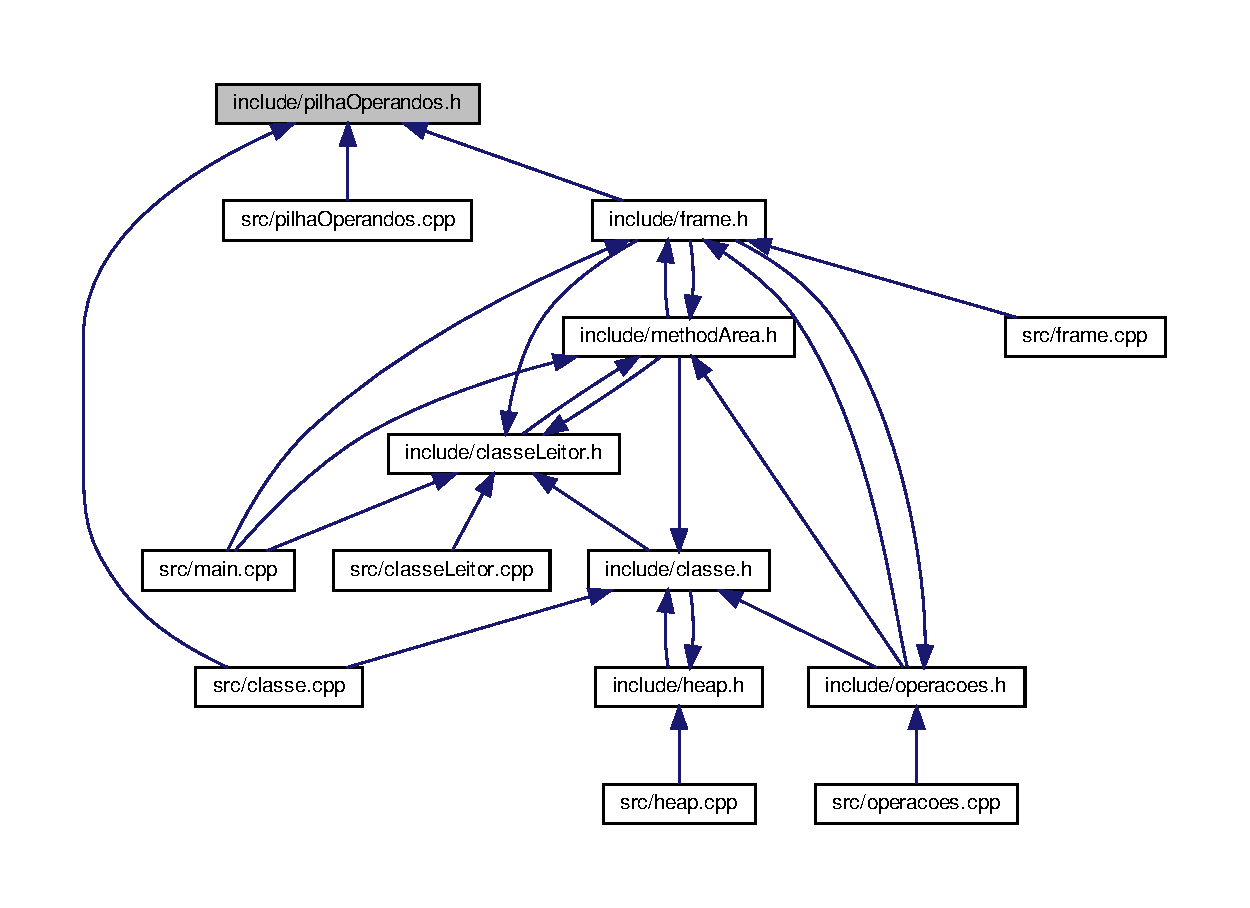
\includegraphics[width=350pt]{pilhaOperandos_8h__dep__incl}
\end{center}
\end{figure}
\subsection*{Estruturas de Dados}
\begin{DoxyCompactItemize}
\item 
class \hyperlink{classPilhaOperandos}{Pilha\+Operandos}
\begin{DoxyCompactList}\small\item\em Classe da pilha de operandos. \end{DoxyCompactList}\end{DoxyCompactItemize}
\subsection*{Macros}
\begin{DoxyCompactItemize}
\item 
\mbox{\Hypertarget{pilhaOperandos_8h_adf770fe2eec438e3758ffe905dbae208}\label{pilhaOperandos_8h_adf770fe2eec438e3758ffe905dbae208}} 
\#define {\bfseries I\+N\+V\+A\+L\+ID}~99
\item 
\mbox{\Hypertarget{pilhaOperandos_8h_a0623cf1b3dda05505734b67f550c53cb}\label{pilhaOperandos_8h_a0623cf1b3dda05505734b67f550c53cb}} 
\#define {\bfseries T\+Y\+P\+E\+\_\+\+N\+O\+T\+\_\+\+S\+ET}~0
\item 
\mbox{\Hypertarget{pilhaOperandos_8h_a56e5f9a95536838408fcca8f22d541b4}\label{pilhaOperandos_8h_a56e5f9a95536838408fcca8f22d541b4}} 
\#define {\bfseries T\+Y\+P\+E\+\_\+\+I\+NT}~1
\item 
\mbox{\Hypertarget{pilhaOperandos_8h_a105c7addfad52601f4d079673eae7982}\label{pilhaOperandos_8h_a105c7addfad52601f4d079673eae7982}} 
\#define {\bfseries T\+Y\+P\+E\+\_\+\+F\+L\+O\+AT}~2
\item 
\mbox{\Hypertarget{pilhaOperandos_8h_a64b164f200989fc609ff40c0e1aa2518}\label{pilhaOperandos_8h_a64b164f200989fc609ff40c0e1aa2518}} 
\#define {\bfseries T\+Y\+P\+E\+\_\+\+L\+O\+NG}~3
\item 
\mbox{\Hypertarget{pilhaOperandos_8h_ac87fa650bc0dcd101b39e15ecdb57477}\label{pilhaOperandos_8h_ac87fa650bc0dcd101b39e15ecdb57477}} 
\#define {\bfseries T\+Y\+P\+E\+\_\+\+D\+O\+U\+B\+LE}~4
\item 
\mbox{\Hypertarget{pilhaOperandos_8h_a375775d23dbf60915db33f1add80c006}\label{pilhaOperandos_8h_a375775d23dbf60915db33f1add80c006}} 
\#define {\bfseries T\+Y\+P\+E\+\_\+\+B\+O\+OL}~5
\item 
\mbox{\Hypertarget{pilhaOperandos_8h_aa1e9e57b2fa5fdc501d79de85b69c986}\label{pilhaOperandos_8h_aa1e9e57b2fa5fdc501d79de85b69c986}} 
\#define {\bfseries T\+Y\+P\+E\+\_\+\+R\+E\+F\+E\+R\+E\+N\+CE}~6
\end{DoxyCompactItemize}


\subsection{Descrição detalhada}
Pilha de operandos. 

Pilha respons�vel por armazenar os operandos da J\+VM 
\hypertarget{attributes_8cpp}{}\section{Referência ao ficheiro src/attributes.cpp}
\label{attributes_8cpp}\index{src/attributes.\+cpp@{src/attributes.\+cpp}}


\hyperlink{attributes_8cpp}{attributes.\+cpp}  


{\ttfamily \#include \char`\"{}attributes.\+h\char`\"{}}\newline
Diagrama de dependências de inclusão para attributes.\+cpp\+:\nopagebreak
\begin{figure}[H]
\begin{center}
\leavevmode
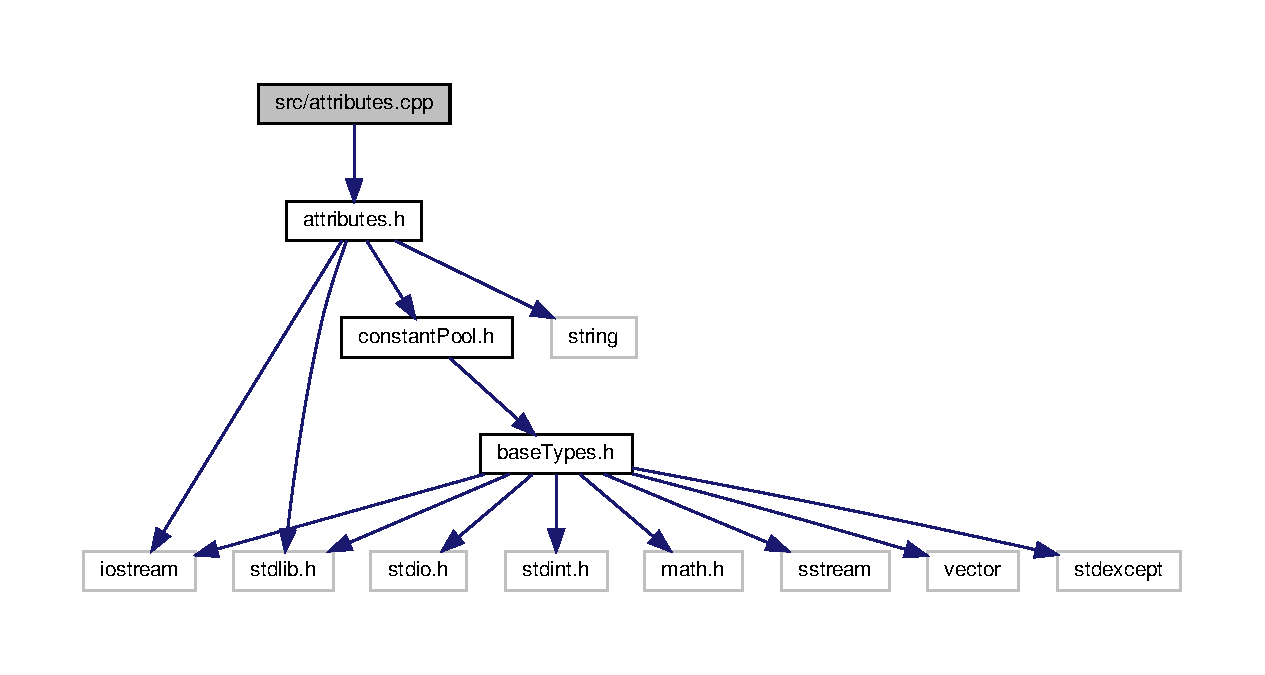
\includegraphics[width=350pt]{attributes_8cpp__incl}
\end{center}
\end{figure}
\subsection*{Funções}
\begin{DoxyCompactItemize}
\item 
\hyperlink{structt__exception__table}{t\+\_\+exception\+\_\+table} $\ast$ \hyperlink{attributes_8cpp_a7996cbd3f25e61cd331881680b847944}{read\+Exception\+Handler} (F\+I\+LE $\ast$fp)
\begin{DoxyCompactList}\small\item\em Função de leitura de exceções. \end{DoxyCompactList}\item 
\hyperlink{uniont__info}{t\+\_\+info} $\ast$ \hyperlink{attributes_8cpp_ac43f8cfd8d4f28e12b2cb8f57209840d}{read\+Attribute\+Info} (F\+I\+LE $\ast$fp, \hyperlink{structcp__info}{cp\+\_\+info} $\ast$cp, unsigned short index, unsigned short length)
\begin{DoxyCompactList}\small\item\em Faz a leitura das informações de um atributo. \end{DoxyCompactList}\item 
\hyperlink{structattribute__info}{attribute\+\_\+info} \hyperlink{attributes_8cpp_a1f014ecafdc1b309e228f89cff54d61e}{read\+Attribute} (F\+I\+LE $\ast$fp, \hyperlink{structcp__info}{cp\+\_\+info} $\ast$cp)
\begin{DoxyCompactList}\small\item\em Faz a leitura de um atributo da constantpool. \end{DoxyCompactList}\item 
\hyperlink{structattribute__info}{attribute\+\_\+info} $\ast$ \hyperlink{attributes_8cpp_abdd523c627a7413b8983f39e42e5ccbc}{read\+Attributes} (F\+I\+LE $\ast$fp, \hyperlink{structcp__info}{cp\+\_\+info} $\ast$cp, int length)
\begin{DoxyCompactList}\small\item\em Faz a leitura de n atributos da constantpool. \end{DoxyCompactList}\item 
void \hyperlink{attributes_8cpp_a6f7d6e88ba48f5785ff23706abb0b030}{print\+Attributes} (\hyperlink{structattribute__info}{attribute\+\_\+info} $\ast$attributes, \hyperlink{structcp__info}{cp\+\_\+info} $\ast$cp, int length)
\begin{DoxyCompactList}\small\item\em Função que imprime na tela informações de n atributos. \end{DoxyCompactList}\item 
void \hyperlink{attributes_8cpp_a7d86b22b81ca886f4457ef3af7a1c5a4}{print\+Attribute} (\hyperlink{structattribute__info}{attribute\+\_\+info} a, \hyperlink{structcp__info}{cp\+\_\+info} $\ast$cp)
\begin{DoxyCompactList}\small\item\em Função que imprime na tela informações de um atributo. \end{DoxyCompactList}\item 
string \hyperlink{attributes_8cpp_a9e977ee82ad332d38ff903bee3228b59}{get\+Mnemonic} (int opcode)
\begin{DoxyCompactList}\small\item\em Returna o nome da operação. \end{DoxyCompactList}\item 
uint32\+\_\+t \hyperlink{attributes_8cpp_ad621a8d31d5756d1512f170c4325bd66}{get\+N\+Bytes\+Value} (uint8\+\_\+t n, unsigned char $\ast$code, int $\ast$index)
\begin{DoxyCompactList}\small\item\em Função para retornar o conteúdo dos próximos n bytes. \end{DoxyCompactList}\item 
void \hyperlink{attributes_8cpp_abc6861f293222814bd642ffc5dfa5777}{get\+Opcode\+Params} (unsigned char $\ast$code, int $\ast$index)
\begin{DoxyCompactList}\small\item\em Função que mostra na tela os parâmetros dos opcodes. \end{DoxyCompactList}\end{DoxyCompactItemize}


\subsection{Descrição detalhada}
\hyperlink{attributes_8cpp}{attributes.\+cpp} 



\subsection{Documentação das funções}
\mbox{\Hypertarget{attributes_8cpp_a9e977ee82ad332d38ff903bee3228b59}\label{attributes_8cpp_a9e977ee82ad332d38ff903bee3228b59}} 
\index{attributes.\+cpp@{attributes.\+cpp}!get\+Mnemonic@{get\+Mnemonic}}
\index{get\+Mnemonic@{get\+Mnemonic}!attributes.\+cpp@{attributes.\+cpp}}
\subsubsection{\texorpdfstring{get\+Mnemonic()}{getMnemonic()}}
{\footnotesize\ttfamily string get\+Mnemonic (\begin{DoxyParamCaption}\item[{int}]{opcode }\end{DoxyParamCaption})}



Returna o nome da operação. 


\begin{DoxyParams}{Parâmetros}
{\em opcode} & Opcode de operações da J\+VM \\
\hline
\end{DoxyParams}
\mbox{\Hypertarget{attributes_8cpp_ad621a8d31d5756d1512f170c4325bd66}\label{attributes_8cpp_ad621a8d31d5756d1512f170c4325bd66}} 
\index{attributes.\+cpp@{attributes.\+cpp}!get\+N\+Bytes\+Value@{get\+N\+Bytes\+Value}}
\index{get\+N\+Bytes\+Value@{get\+N\+Bytes\+Value}!attributes.\+cpp@{attributes.\+cpp}}
\subsubsection{\texorpdfstring{get\+N\+Bytes\+Value()}{getNBytesValue()}}
{\footnotesize\ttfamily uint32\+\_\+t get\+N\+Bytes\+Value (\begin{DoxyParamCaption}\item[{uint8\+\_\+t}]{n,  }\item[{unsigned char $\ast$}]{code,  }\item[{int $\ast$}]{index }\end{DoxyParamCaption})}



Função para retornar o conteúdo dos próximos n bytes. 


\begin{DoxyParams}{Parâmetros}
{\em n} & Número de bytes a serem lidos. \\
\hline
{\em code} & Ponteiro pra um vetor de bytes. \\
\hline
{\em index} & Posição do opcode no vetor. \\
\hline
\end{DoxyParams}
\mbox{\Hypertarget{attributes_8cpp_abc6861f293222814bd642ffc5dfa5777}\label{attributes_8cpp_abc6861f293222814bd642ffc5dfa5777}} 
\index{attributes.\+cpp@{attributes.\+cpp}!get\+Opcode\+Params@{get\+Opcode\+Params}}
\index{get\+Opcode\+Params@{get\+Opcode\+Params}!attributes.\+cpp@{attributes.\+cpp}}
\subsubsection{\texorpdfstring{get\+Opcode\+Params()}{getOpcodeParams()}}
{\footnotesize\ttfamily void get\+Opcode\+Params (\begin{DoxyParamCaption}\item[{unsigned char $\ast$}]{code,  }\item[{int $\ast$}]{index }\end{DoxyParamCaption})}



Função que mostra na tela os parâmetros dos opcodes. 


\begin{DoxyParams}{Parâmetros}
{\em code} & Pointer of bytes wich are code and your arg. Ponteiro para vetor de bytes do código e seus parâemtros. \\
\hline
{\em index} & Posição na constantpool. \\
\hline
\end{DoxyParams}
\mbox{\Hypertarget{attributes_8cpp_a7d86b22b81ca886f4457ef3af7a1c5a4}\label{attributes_8cpp_a7d86b22b81ca886f4457ef3af7a1c5a4}} 
\index{attributes.\+cpp@{attributes.\+cpp}!print\+Attribute@{print\+Attribute}}
\index{print\+Attribute@{print\+Attribute}!attributes.\+cpp@{attributes.\+cpp}}
\subsubsection{\texorpdfstring{print\+Attribute()}{printAttribute()}}
{\footnotesize\ttfamily void print\+Attribute (\begin{DoxyParamCaption}\item[{\hyperlink{structattribute__info}{attribute\+\_\+info}}]{a,  }\item[{\hyperlink{structcp__info}{cp\+\_\+info} $\ast$}]{cp }\end{DoxyParamCaption})}



Função que imprime na tela informações de um atributo. 


\begin{DoxyParams}{Parâmetros}
{\em cp} & Poteiro pra constant pool. \\
\hline
\end{DoxyParams}
\mbox{\Hypertarget{attributes_8cpp_a6f7d6e88ba48f5785ff23706abb0b030}\label{attributes_8cpp_a6f7d6e88ba48f5785ff23706abb0b030}} 
\index{attributes.\+cpp@{attributes.\+cpp}!print\+Attributes@{print\+Attributes}}
\index{print\+Attributes@{print\+Attributes}!attributes.\+cpp@{attributes.\+cpp}}
\subsubsection{\texorpdfstring{print\+Attributes()}{printAttributes()}}
{\footnotesize\ttfamily void print\+Attributes (\begin{DoxyParamCaption}\item[{\hyperlink{structattribute__info}{attribute\+\_\+info} $\ast$}]{attributes,  }\item[{\hyperlink{structcp__info}{cp\+\_\+info} $\ast$}]{cp,  }\item[{int}]{length }\end{DoxyParamCaption})}



Função que imprime na tela informações de n atributos. 


\begin{DoxyParams}{Parâmetros}
{\em attributes} & Pointer to struct of types att. \\
\hline
{\em cp} & Poteiro pra constant pool. \\
\hline
{\em length} & Number of times of the function print\+Attribute gonna be called. \\
\hline
\end{DoxyParams}
\mbox{\Hypertarget{attributes_8cpp_a1f014ecafdc1b309e228f89cff54d61e}\label{attributes_8cpp_a1f014ecafdc1b309e228f89cff54d61e}} 
\index{attributes.\+cpp@{attributes.\+cpp}!read\+Attribute@{read\+Attribute}}
\index{read\+Attribute@{read\+Attribute}!attributes.\+cpp@{attributes.\+cpp}}
\subsubsection{\texorpdfstring{read\+Attribute()}{readAttribute()}}
{\footnotesize\ttfamily \hyperlink{structattribute__info}{attribute\+\_\+info} read\+Attribute (\begin{DoxyParamCaption}\item[{F\+I\+LE $\ast$}]{fp,  }\item[{\hyperlink{structcp__info}{cp\+\_\+info} $\ast$}]{cp }\end{DoxyParamCaption})}



Faz a leitura de um atributo da constantpool. 


\begin{DoxyParams}{Parâmetros}
{\em fp} & Ponteiro pro arquivo .class. \\
\hline
{\em cp} & Pointeiro pra constantpool. \\
\hline
\end{DoxyParams}
\mbox{\Hypertarget{attributes_8cpp_ac43f8cfd8d4f28e12b2cb8f57209840d}\label{attributes_8cpp_ac43f8cfd8d4f28e12b2cb8f57209840d}} 
\index{attributes.\+cpp@{attributes.\+cpp}!read\+Attribute\+Info@{read\+Attribute\+Info}}
\index{read\+Attribute\+Info@{read\+Attribute\+Info}!attributes.\+cpp@{attributes.\+cpp}}
\subsubsection{\texorpdfstring{read\+Attribute\+Info()}{readAttributeInfo()}}
{\footnotesize\ttfamily \hyperlink{uniont__info}{t\+\_\+info} $\ast$ read\+Attribute\+Info (\begin{DoxyParamCaption}\item[{F\+I\+LE $\ast$}]{fp,  }\item[{\hyperlink{structcp__info}{cp\+\_\+info} $\ast$}]{cp,  }\item[{unsigned short}]{index,  }\item[{unsigned short}]{length }\end{DoxyParamCaption})}



Faz a leitura das informações de um atributo. 


\begin{DoxyParams}{Parâmetros}
{\em fp} & Ponteirp para arquivo .class. \\
\hline
{\em cp} & Ponteiro pra constantpool. \\
\hline
{\em Posição} & do atributo na constantpool. \\
\hline
{\em Tamanho} & em bytes do atributo a ser lido. \\
\hline
\end{DoxyParams}
\mbox{\Hypertarget{attributes_8cpp_abdd523c627a7413b8983f39e42e5ccbc}\label{attributes_8cpp_abdd523c627a7413b8983f39e42e5ccbc}} 
\index{attributes.\+cpp@{attributes.\+cpp}!read\+Attributes@{read\+Attributes}}
\index{read\+Attributes@{read\+Attributes}!attributes.\+cpp@{attributes.\+cpp}}
\subsubsection{\texorpdfstring{read\+Attributes()}{readAttributes()}}
{\footnotesize\ttfamily \hyperlink{structattribute__info}{attribute\+\_\+info} $\ast$ read\+Attributes (\begin{DoxyParamCaption}\item[{F\+I\+LE $\ast$}]{fp,  }\item[{\hyperlink{structcp__info}{cp\+\_\+info} $\ast$}]{cp,  }\item[{int}]{length }\end{DoxyParamCaption})}



Faz a leitura de n atributos da constantpool. 


\begin{DoxyParams}{Parâmetros}
{\em fp} & Ponteiro pro arquivo .class. \\
\hline
{\em cp} & Poteiro pra constant pool. \\
\hline
{\em length} & Número de atributos. \\
\hline
\end{DoxyParams}
\mbox{\Hypertarget{attributes_8cpp_a7996cbd3f25e61cd331881680b847944}\label{attributes_8cpp_a7996cbd3f25e61cd331881680b847944}} 
\index{attributes.\+cpp@{attributes.\+cpp}!read\+Exception\+Handler@{read\+Exception\+Handler}}
\index{read\+Exception\+Handler@{read\+Exception\+Handler}!attributes.\+cpp@{attributes.\+cpp}}
\subsubsection{\texorpdfstring{read\+Exception\+Handler()}{readExceptionHandler()}}
{\footnotesize\ttfamily \hyperlink{structt__exception__table}{t\+\_\+exception\+\_\+table} $\ast$ read\+Exception\+Handler (\begin{DoxyParamCaption}\item[{F\+I\+LE $\ast$}]{fp }\end{DoxyParamCaption})}



Função de leitura de exceções. 


\begin{DoxyParams}{Parâmetros}
{\em fp} & Ponteiro para arquivo tipo .class \\
\hline
\end{DoxyParams}

\hypertarget{baseTypes_8cpp}{}\section{Referência ao ficheiro src/base\+Types.cpp}
\label{baseTypes_8cpp}\index{src/base\+Types.\+cpp@{src/base\+Types.\+cpp}}


basetypes.\+cpp  


{\ttfamily \#include \char`\"{}base\+Types.\+h\char`\"{}}\newline
Diagrama de dependências de inclusão para base\+Types.\+cpp\+:\nopagebreak
\begin{figure}[H]
\begin{center}
\leavevmode
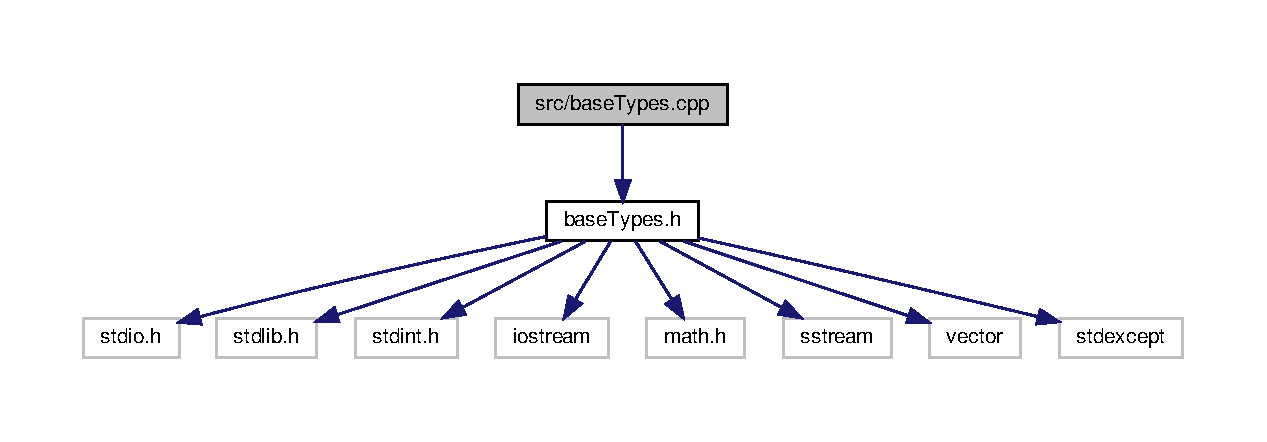
\includegraphics[width=350pt]{baseTypes_8cpp__incl}
\end{center}
\end{figure}
\subsection*{Funções}
\begin{DoxyCompactItemize}
\item 
U2 \hyperlink{baseTypes_8cpp_a81f8cf10d3f1ee282c2f124ebf00b718}{read\+U2} (F\+I\+LE $\ast$fp)
\begin{DoxyCompactList}\small\item\em Função para ler 2 bytes do arquivo .class. \end{DoxyCompactList}\item 
U1 \hyperlink{baseTypes_8cpp_a8a134c72da9699c32dbec57627955328}{read\+U1} (F\+I\+LE $\ast$fp)
\begin{DoxyCompactList}\small\item\em Função para ler 1 byte do arquivo .class. \end{DoxyCompactList}\item 
U1 $\ast$ \hyperlink{baseTypes_8cpp_aa8607f57d05a9bb119626bfb04410131}{read\+U\+T\+F8} (F\+I\+LE $\ast$fp, int size)
\begin{DoxyCompactList}\small\item\em Função para ler os bytes de uma string U\+T\+F-\/8. \end{DoxyCompactList}\item 
U4 \hyperlink{baseTypes_8cpp_a836a4be80a9f428623a68e687e6c30c6}{read\+U4} (F\+I\+LE $\ast$fp)
\begin{DoxyCompactList}\small\item\em Função para ler 4 bytes do arquivo .class. \end{DoxyCompactList}\item 
string \hyperlink{baseTypes_8cpp_a22f1f8c2b398f9db39f18565b36986f1}{show\+U\+T\+F8} (unsigned char $\ast$s, int size)
\begin{DoxyCompactList}\small\item\em Função para montar e mostrar a uma string U\+T\+F-\/8. \end{DoxyCompactList}\item 
string \hyperlink{baseTypes_8cpp_a35ee76375b4843822c2f7dec234ae0eb}{double\+\_\+to\+\_\+string} (double d)
\begin{DoxyCompactList}\small\item\em Função para converter double para string. \end{DoxyCompactList}\item 
int \hyperlink{baseTypes_8cpp_a871378ebfdafb26a99e3108b15e70a98}{check\+Float} (float f)
\begin{DoxyCompactList}\small\item\em Função para verificar NaN e infinito. \end{DoxyCompactList}\item 
int \hyperlink{baseTypes_8cpp_a7e9defed00ed2d5b820a06a3ecbfffaf}{check\+Double} (double d)
\begin{DoxyCompactList}\small\item\em Função para verificar NaN e infinito. \end{DoxyCompactList}\item 
string \hyperlink{baseTypes_8cpp_a6144b769255fad600d6a8339de3c637c}{float\+\_\+to\+\_\+string} (float f)
\begin{DoxyCompactList}\small\item\em Função para converter float para string. \end{DoxyCompactList}\item 
long \hyperlink{baseTypes_8cpp_a5b4ee2146dd5beafbac7709a37bdbbd2}{u4\+\_\+to\+\_\+long} (\hyperlink{unionClassLoaderType}{Class\+Loader\+Type} high, \hyperlink{unionClassLoaderType}{Class\+Loader\+Type} low)
\begin{DoxyCompactList}\small\item\em Function to convert 8 bytes to a long. \end{DoxyCompactList}\item 
double \hyperlink{baseTypes_8cpp_a51bdc30e142e0a9d888eb56ce9b5484b}{u4\+\_\+to\+\_\+double} (\hyperlink{unionClassLoaderType}{Class\+Loader\+Type} high, \hyperlink{unionClassLoaderType}{Class\+Loader\+Type} low)
\begin{DoxyCompactList}\small\item\em Function to convert 8 bytes to a double. \end{DoxyCompactList}\item 
float \hyperlink{baseTypes_8cpp_a0f3ffb86bcc68531d481dd68c556b086}{u4\+\_\+to\+\_\+float} (\hyperlink{unionClassLoaderType}{Class\+Loader\+Type} in)
\begin{DoxyCompactList}\small\item\em Function to convert 4 bytes to a float. \end{DoxyCompactList}\end{DoxyCompactItemize}


\subsection{Descrição detalhada}
basetypes.\+cpp 



\subsection{Documentação das funções}
\mbox{\Hypertarget{baseTypes_8cpp_a7e9defed00ed2d5b820a06a3ecbfffaf}\label{baseTypes_8cpp_a7e9defed00ed2d5b820a06a3ecbfffaf}} 
\index{base\+Types.\+cpp@{base\+Types.\+cpp}!check\+Double@{check\+Double}}
\index{check\+Double@{check\+Double}!base\+Types.\+cpp@{base\+Types.\+cpp}}
\subsubsection{\texorpdfstring{check\+Double()}{checkDouble()}}
{\footnotesize\ttfamily int check\+Double (\begin{DoxyParamCaption}\item[{double}]{d }\end{DoxyParamCaption})}



Função para verificar NaN e infinito. 


\begin{DoxyParams}{Parâmetros}
{\em double} & Number to be checked. \\
\hline
\end{DoxyParams}
\mbox{\Hypertarget{baseTypes_8cpp_a871378ebfdafb26a99e3108b15e70a98}\label{baseTypes_8cpp_a871378ebfdafb26a99e3108b15e70a98}} 
\index{base\+Types.\+cpp@{base\+Types.\+cpp}!check\+Float@{check\+Float}}
\index{check\+Float@{check\+Float}!base\+Types.\+cpp@{base\+Types.\+cpp}}
\subsubsection{\texorpdfstring{check\+Float()}{checkFloat()}}
{\footnotesize\ttfamily int check\+Float (\begin{DoxyParamCaption}\item[{float}]{f }\end{DoxyParamCaption})}



Função para verificar NaN e infinito. 


\begin{DoxyParams}{Parâmetros}
{\em float} & Número a ser verificado. \\
\hline
\end{DoxyParams}
\mbox{\Hypertarget{baseTypes_8cpp_a35ee76375b4843822c2f7dec234ae0eb}\label{baseTypes_8cpp_a35ee76375b4843822c2f7dec234ae0eb}} 
\index{base\+Types.\+cpp@{base\+Types.\+cpp}!double\+\_\+to\+\_\+string@{double\+\_\+to\+\_\+string}}
\index{double\+\_\+to\+\_\+string@{double\+\_\+to\+\_\+string}!base\+Types.\+cpp@{base\+Types.\+cpp}}
\subsubsection{\texorpdfstring{double\+\_\+to\+\_\+string()}{double\_to\_string()}}
{\footnotesize\ttfamily string double\+\_\+to\+\_\+string (\begin{DoxyParamCaption}\item[{double}]{d }\end{DoxyParamCaption})}



Função para converter double para string. 


\begin{DoxyParams}{Parâmetros}
{\em double} & Número a ser convertido. \\
\hline
\end{DoxyParams}
\mbox{\Hypertarget{baseTypes_8cpp_a6144b769255fad600d6a8339de3c637c}\label{baseTypes_8cpp_a6144b769255fad600d6a8339de3c637c}} 
\index{base\+Types.\+cpp@{base\+Types.\+cpp}!float\+\_\+to\+\_\+string@{float\+\_\+to\+\_\+string}}
\index{float\+\_\+to\+\_\+string@{float\+\_\+to\+\_\+string}!base\+Types.\+cpp@{base\+Types.\+cpp}}
\subsubsection{\texorpdfstring{float\+\_\+to\+\_\+string()}{float\_to\_string()}}
{\footnotesize\ttfamily string float\+\_\+to\+\_\+string (\begin{DoxyParamCaption}\item[{float}]{f }\end{DoxyParamCaption})}



Função para converter float para string. 


\begin{DoxyParams}{Parâmetros}
{\em float} & Número a ser convertido. \\
\hline
\end{DoxyParams}
\mbox{\Hypertarget{baseTypes_8cpp_a8a134c72da9699c32dbec57627955328}\label{baseTypes_8cpp_a8a134c72da9699c32dbec57627955328}} 
\index{base\+Types.\+cpp@{base\+Types.\+cpp}!read\+U1@{read\+U1}}
\index{read\+U1@{read\+U1}!base\+Types.\+cpp@{base\+Types.\+cpp}}
\subsubsection{\texorpdfstring{read\+U1()}{readU1()}}
{\footnotesize\ttfamily U1 read\+U1 (\begin{DoxyParamCaption}\item[{F\+I\+LE $\ast$}]{fp }\end{DoxyParamCaption})}



Função para ler 1 byte do arquivo .class. 


\begin{DoxyParams}{Parâmetros}
{\em fp.} & Ponteiro pro arquivo .class \\
\hline
\end{DoxyParams}
\mbox{\Hypertarget{baseTypes_8cpp_a81f8cf10d3f1ee282c2f124ebf00b718}\label{baseTypes_8cpp_a81f8cf10d3f1ee282c2f124ebf00b718}} 
\index{base\+Types.\+cpp@{base\+Types.\+cpp}!read\+U2@{read\+U2}}
\index{read\+U2@{read\+U2}!base\+Types.\+cpp@{base\+Types.\+cpp}}
\subsubsection{\texorpdfstring{read\+U2()}{readU2()}}
{\footnotesize\ttfamily U2 read\+U2 (\begin{DoxyParamCaption}\item[{F\+I\+LE $\ast$}]{fp }\end{DoxyParamCaption})}



Função para ler 2 bytes do arquivo .class. 


\begin{DoxyParams}{Parâmetros}
{\em fp.} & Ponteiro pro arquivo .class \\
\hline
\end{DoxyParams}
\mbox{\Hypertarget{baseTypes_8cpp_a836a4be80a9f428623a68e687e6c30c6}\label{baseTypes_8cpp_a836a4be80a9f428623a68e687e6c30c6}} 
\index{base\+Types.\+cpp@{base\+Types.\+cpp}!read\+U4@{read\+U4}}
\index{read\+U4@{read\+U4}!base\+Types.\+cpp@{base\+Types.\+cpp}}
\subsubsection{\texorpdfstring{read\+U4()}{readU4()}}
{\footnotesize\ttfamily U4 read\+U4 (\begin{DoxyParamCaption}\item[{F\+I\+LE $\ast$}]{fp }\end{DoxyParamCaption})}



Função para ler 4 bytes do arquivo .class. 


\begin{DoxyParams}{Parâmetros}
{\em fp.} & Ponteiro pro arquivo .class \\
\hline
\end{DoxyParams}
\mbox{\Hypertarget{baseTypes_8cpp_aa8607f57d05a9bb119626bfb04410131}\label{baseTypes_8cpp_aa8607f57d05a9bb119626bfb04410131}} 
\index{base\+Types.\+cpp@{base\+Types.\+cpp}!read\+U\+T\+F8@{read\+U\+T\+F8}}
\index{read\+U\+T\+F8@{read\+U\+T\+F8}!base\+Types.\+cpp@{base\+Types.\+cpp}}
\subsubsection{\texorpdfstring{read\+U\+T\+F8()}{readUTF8()}}
{\footnotesize\ttfamily U1 $\ast$ read\+U\+T\+F8 (\begin{DoxyParamCaption}\item[{F\+I\+LE $\ast$}]{fp,  }\item[{int}]{size }\end{DoxyParamCaption})}



Função para ler os bytes de uma string U\+T\+F-\/8. 


\begin{DoxyParams}{Parâmetros}
{\em fp.} & Ponteiro pro arquivo .class \\
\hline
{\em size} & Tamanho que será alocado para a string. \\
\hline
\end{DoxyParams}
\mbox{\Hypertarget{baseTypes_8cpp_a22f1f8c2b398f9db39f18565b36986f1}\label{baseTypes_8cpp_a22f1f8c2b398f9db39f18565b36986f1}} 
\index{base\+Types.\+cpp@{base\+Types.\+cpp}!show\+U\+T\+F8@{show\+U\+T\+F8}}
\index{show\+U\+T\+F8@{show\+U\+T\+F8}!base\+Types.\+cpp@{base\+Types.\+cpp}}
\subsubsection{\texorpdfstring{show\+U\+T\+F8()}{showUTF8()}}
{\footnotesize\ttfamily string show\+U\+T\+F8 (\begin{DoxyParamCaption}\item[{unsigned char $\ast$}]{s,  }\item[{int}]{size }\end{DoxyParamCaption})}



Função para montar e mostrar a uma string U\+T\+F-\/8. 


\begin{DoxyParams}{Parâmetros}
{\em s} & Ponteiro para a posição inicial de uam string Unicode. \\
\hline
{\em size} & Tamanho da string a ser impressa. \\
\hline
\end{DoxyParams}
\mbox{\Hypertarget{baseTypes_8cpp_a51bdc30e142e0a9d888eb56ce9b5484b}\label{baseTypes_8cpp_a51bdc30e142e0a9d888eb56ce9b5484b}} 
\index{base\+Types.\+cpp@{base\+Types.\+cpp}!u4\+\_\+to\+\_\+double@{u4\+\_\+to\+\_\+double}}
\index{u4\+\_\+to\+\_\+double@{u4\+\_\+to\+\_\+double}!base\+Types.\+cpp@{base\+Types.\+cpp}}
\subsubsection{\texorpdfstring{u4\+\_\+to\+\_\+double()}{u4\_to\_double()}}
{\footnotesize\ttfamily double u4\+\_\+to\+\_\+double (\begin{DoxyParamCaption}\item[{\hyperlink{unionClassLoaderType}{Class\+Loader\+Type}}]{high,  }\item[{\hyperlink{unionClassLoaderType}{Class\+Loader\+Type}}]{low }\end{DoxyParamCaption})}



Function to convert 8 bytes to a double. 


\begin{DoxyParams}{Parâmetros}
{\em high} & Four most significant bytes to be converted. \\
\hline
{\em low} & Four last significant bytes to be converted. \\
\hline
\end{DoxyParams}
\mbox{\Hypertarget{baseTypes_8cpp_a0f3ffb86bcc68531d481dd68c556b086}\label{baseTypes_8cpp_a0f3ffb86bcc68531d481dd68c556b086}} 
\index{base\+Types.\+cpp@{base\+Types.\+cpp}!u4\+\_\+to\+\_\+float@{u4\+\_\+to\+\_\+float}}
\index{u4\+\_\+to\+\_\+float@{u4\+\_\+to\+\_\+float}!base\+Types.\+cpp@{base\+Types.\+cpp}}
\subsubsection{\texorpdfstring{u4\+\_\+to\+\_\+float()}{u4\_to\_float()}}
{\footnotesize\ttfamily float u4\+\_\+to\+\_\+float (\begin{DoxyParamCaption}\item[{\hyperlink{unionClassLoaderType}{Class\+Loader\+Type}}]{in }\end{DoxyParamCaption})}



Function to convert 4 bytes to a float. 


\begin{DoxyParams}{Parâmetros}
{\em in} & Four bytes to be converted. \\
\hline
\end{DoxyParams}
\mbox{\Hypertarget{baseTypes_8cpp_a5b4ee2146dd5beafbac7709a37bdbbd2}\label{baseTypes_8cpp_a5b4ee2146dd5beafbac7709a37bdbbd2}} 
\index{base\+Types.\+cpp@{base\+Types.\+cpp}!u4\+\_\+to\+\_\+long@{u4\+\_\+to\+\_\+long}}
\index{u4\+\_\+to\+\_\+long@{u4\+\_\+to\+\_\+long}!base\+Types.\+cpp@{base\+Types.\+cpp}}
\subsubsection{\texorpdfstring{u4\+\_\+to\+\_\+long()}{u4\_to\_long()}}
{\footnotesize\ttfamily long u4\+\_\+to\+\_\+long (\begin{DoxyParamCaption}\item[{\hyperlink{unionClassLoaderType}{Class\+Loader\+Type}}]{high,  }\item[{\hyperlink{unionClassLoaderType}{Class\+Loader\+Type}}]{low }\end{DoxyParamCaption})}



Function to convert 8 bytes to a long. 


\begin{DoxyParams}{Parâmetros}
{\em high} & Four most significant bytes to be converted. \\
\hline
{\em low} & Four last significant bytes to be converted. \\
\hline
\end{DoxyParams}

\hypertarget{classe_8cpp}{}\section{Referência ao ficheiro src/classe.cpp}
\label{classe_8cpp}\index{src/classe.\+cpp@{src/classe.\+cpp}}


\hyperlink{classe_8cpp}{classe.\+cpp}  


{\ttfamily \#include \char`\"{}classe.\+h\char`\"{}}\newline
{\ttfamily \#include \char`\"{}pilha\+Operandos.\+h\char`\"{}}\newline
Diagrama de dependências de inclusão para classe.\+cpp\+:\nopagebreak
\begin{figure}[H]
\begin{center}
\leavevmode
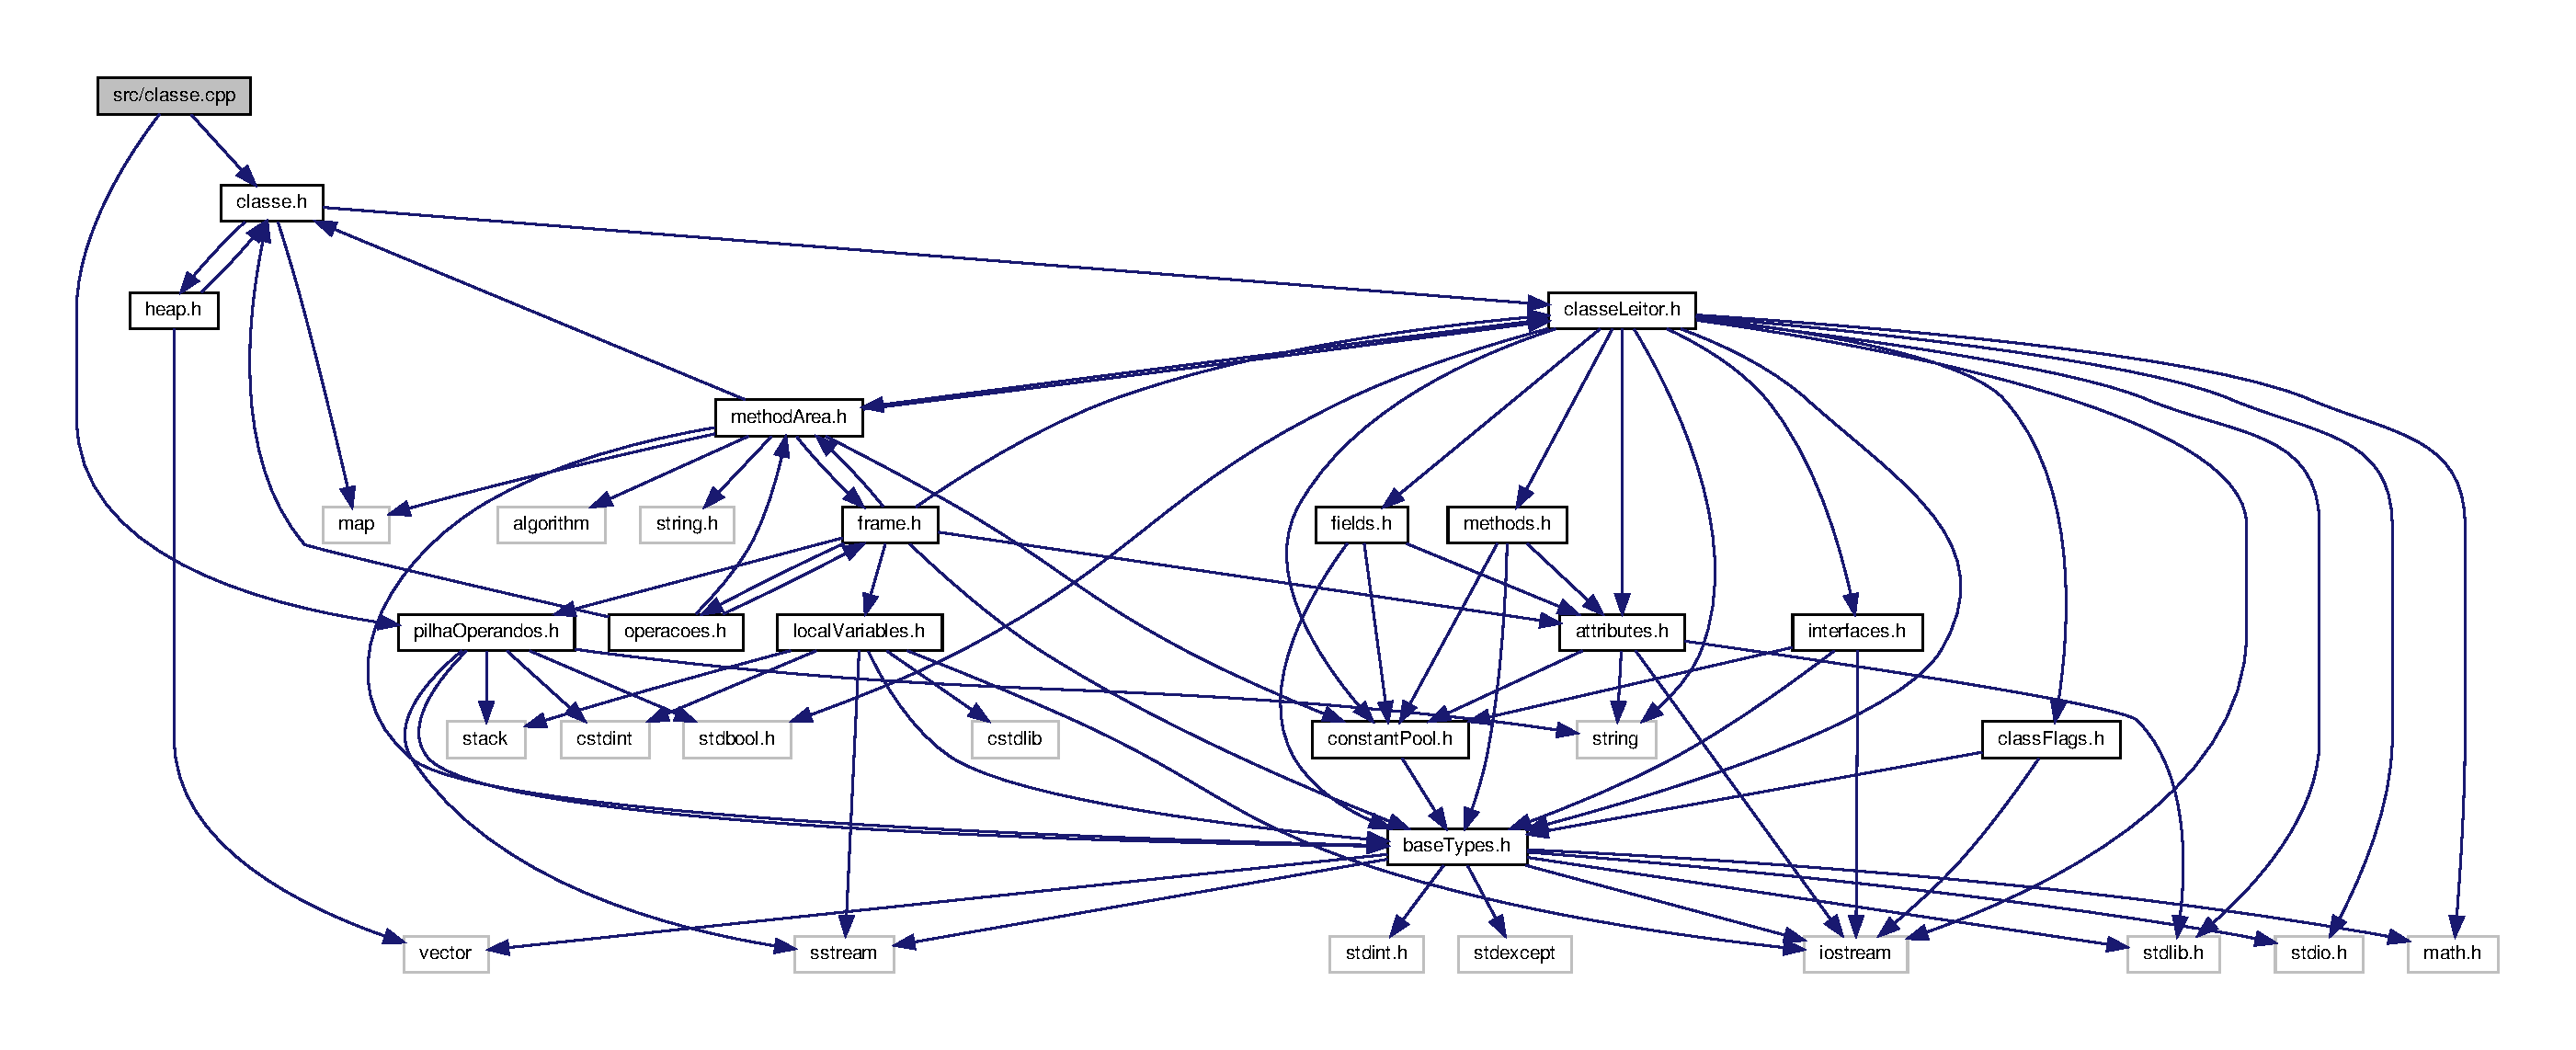
\includegraphics[width=350pt]{classe_8cpp__incl}
\end{center}
\end{figure}


\subsection{Descrição detalhada}
\hyperlink{classe_8cpp}{classe.\+cpp} 


\hypertarget{classFlags_8cpp}{}\section{Referência ao ficheiro src/class\+Flags.cpp}
\label{classFlags_8cpp}\index{src/class\+Flags.\+cpp@{src/class\+Flags.\+cpp}}


Class\+Flags.\+cpp.  


{\ttfamily \#include \char`\"{}class\+Flags.\+h\char`\"{}}\newline
Diagrama de dependências de inclusão para class\+Flags.\+cpp\+:\nopagebreak
\begin{figure}[H]
\begin{center}
\leavevmode
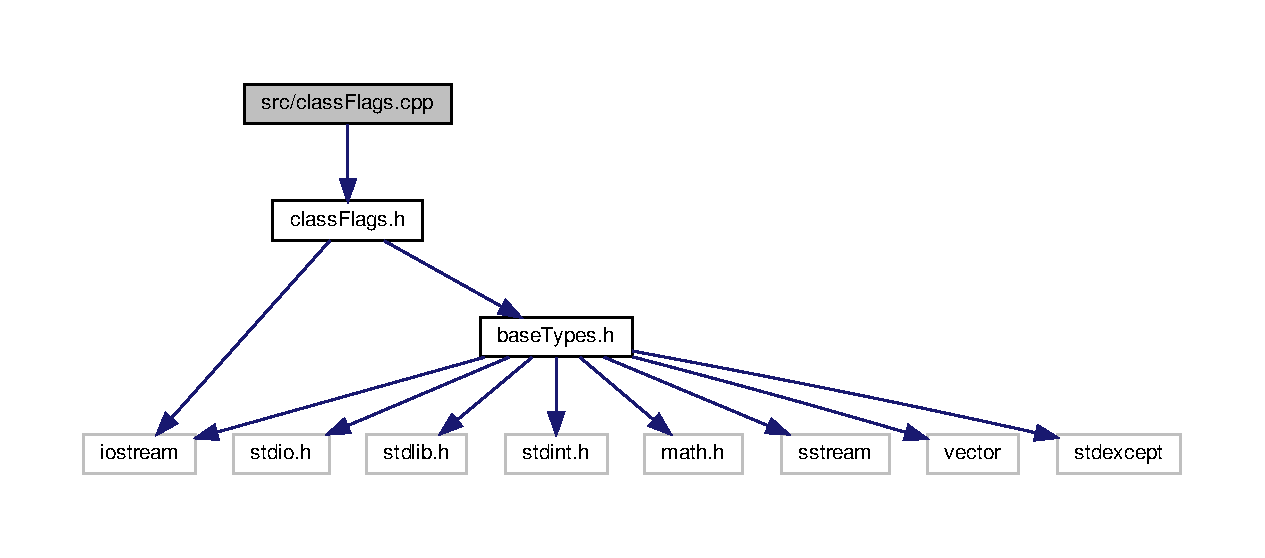
\includegraphics[width=350pt]{classFlags_8cpp__incl}
\end{center}
\end{figure}
\subsection*{Funções}
\begin{DoxyCompactItemize}
\item 
void \hyperlink{classFlags_8cpp_a99a1809d6be6fe7e8b56fa56e2da57ae}{show\+Flags} (U2 access\+Flags)
\begin{DoxyCompactList}\small\item\em Função que mostra as flags de acesso para os usuários. \end{DoxyCompactList}\end{DoxyCompactItemize}


\subsection{Descrição detalhada}
Class\+Flags.\+cpp. 



\subsection{Documentação das funções}
\mbox{\Hypertarget{classFlags_8cpp_a99a1809d6be6fe7e8b56fa56e2da57ae}\label{classFlags_8cpp_a99a1809d6be6fe7e8b56fa56e2da57ae}} 
\index{class\+Flags.\+cpp@{class\+Flags.\+cpp}!show\+Flags@{show\+Flags}}
\index{show\+Flags@{show\+Flags}!class\+Flags.\+cpp@{class\+Flags.\+cpp}}
\subsubsection{\texorpdfstring{show\+Flags()}{showFlags()}}
{\footnotesize\ttfamily void show\+Flags (\begin{DoxyParamCaption}\item[{U2}]{flags }\end{DoxyParamCaption})}



Função que mostra as flags de acesso para os usuários. 

Função que mostra as flags de acesso para os usuários 
\begin{DoxyParams}{Parâmetros}
{\em flags} & Valor hexadecimal das flags\\
\hline
{\em flags} & Valor hexadecimal das flags \\
\hline
\end{DoxyParams}

\hypertarget{constantPool_8cpp}{}\section{Referência ao ficheiro src/constant\+Pool.cpp}
\label{constantPool_8cpp}\index{src/constant\+Pool.\+cpp@{src/constant\+Pool.\+cpp}}


\hyperlink{constantPool_8cpp}{constant\+Pool.\+cpp}  


{\ttfamily \#include \char`\"{}constant\+Pool.\+h\char`\"{}}\newline
Diagrama de dependências de inclusão para constant\+Pool.\+cpp\+:\nopagebreak
\begin{figure}[H]
\begin{center}
\leavevmode
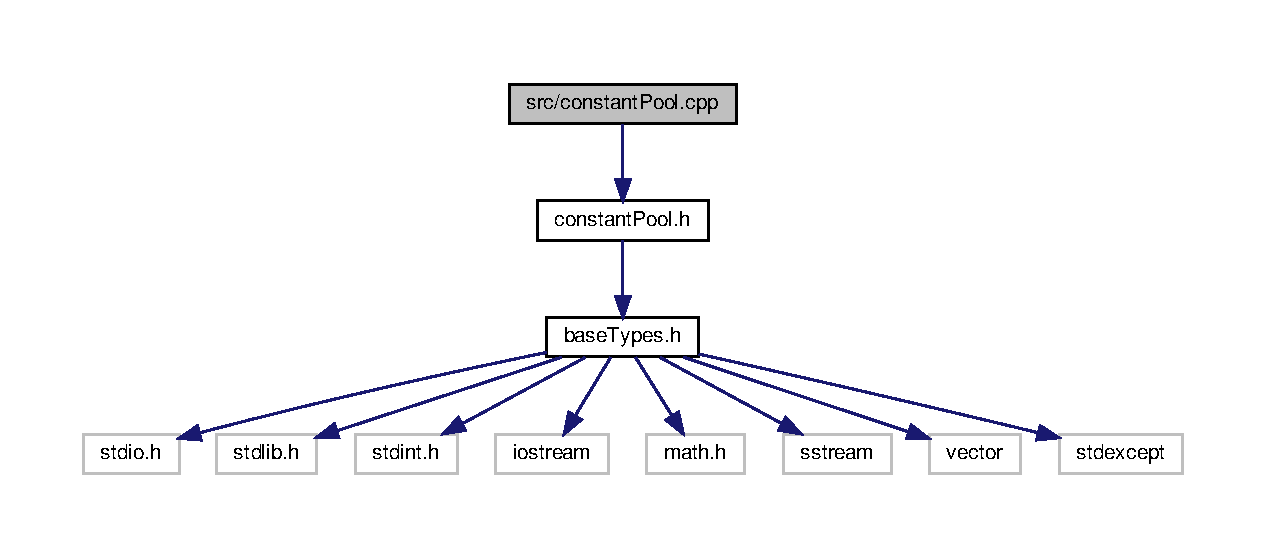
\includegraphics[width=350pt]{constantPool_8cpp__incl}
\end{center}
\end{figure}
\subsection*{Funções}
\begin{DoxyCompactItemize}
\item 
int \hyperlink{constantPool_8cpp_aeed51c70547d5b043643766a20b34127}{load\+Constant\+Pool} (\hyperlink{structcp__info}{cp\+\_\+info} $\ast$constant\+Pool, int length\+CP, F\+I\+LE $\ast$fp)
\begin{DoxyCompactList}\small\item\em Carrega o pool de constantes. \end{DoxyCompactList}\item 
string \hyperlink{constantPool_8cpp_a3b41d9a03a7d0060e40c3135a4d341b9}{dereference\+Index} (\hyperlink{structcp__info}{cp\+\_\+info} $\ast$cp, U2 index)
\begin{DoxyCompactList}\small\item\em Retorna os dados no índice. \end{DoxyCompactList}\item 
void \hyperlink{constantPool_8cpp_a885fc96896e2694a220fb936c97b929f}{print\+Constant\+Pool} (\hyperlink{structcp__info}{cp\+\_\+info} $\ast$constant\+Pool, int length\+CP)
\begin{DoxyCompactList}\small\item\em Imprime o pool de constantes. \end{DoxyCompactList}\end{DoxyCompactItemize}


\subsection{Descrição detalhada}
\hyperlink{constantPool_8cpp}{constant\+Pool.\+cpp} 

Este módulo contém as funções necessárias para a manipulação do pool de constantes. 

\subsection{Documentação das funções}
\mbox{\Hypertarget{constantPool_8cpp_a3b41d9a03a7d0060e40c3135a4d341b9}\label{constantPool_8cpp_a3b41d9a03a7d0060e40c3135a4d341b9}} 
\index{constant\+Pool.\+cpp@{constant\+Pool.\+cpp}!dereference\+Index@{dereference\+Index}}
\index{dereference\+Index@{dereference\+Index}!constant\+Pool.\+cpp@{constant\+Pool.\+cpp}}
\subsubsection{\texorpdfstring{dereference\+Index()}{dereferenceIndex()}}
{\footnotesize\ttfamily string dereference\+Index (\begin{DoxyParamCaption}\item[{\hyperlink{structcp__info}{cp\+\_\+info} $\ast$}]{cp,  }\item[{U2}]{index }\end{DoxyParamCaption})}



Retorna os dados no índice. 


\begin{DoxyParams}{Parâmetros}
{\em cp} & -\/ um ponteiro para o pool de contantes \\
\hline
{\em index} & -\/ um índice para a posição no pool de constantes \\
\hline
\end{DoxyParams}
\hypertarget{constantPool_8cpp_desc}{}\subsection{Descrição}\label{constantPool_8cpp_desc}
Função responsável por obter os dados correspondentes ao índice informado \mbox{\Hypertarget{constantPool_8cpp_aeed51c70547d5b043643766a20b34127}\label{constantPool_8cpp_aeed51c70547d5b043643766a20b34127}} 
\index{constant\+Pool.\+cpp@{constant\+Pool.\+cpp}!load\+Constant\+Pool@{load\+Constant\+Pool}}
\index{load\+Constant\+Pool@{load\+Constant\+Pool}!constant\+Pool.\+cpp@{constant\+Pool.\+cpp}}
\subsubsection{\texorpdfstring{load\+Constant\+Pool()}{loadConstantPool()}}
{\footnotesize\ttfamily int load\+Constant\+Pool (\begin{DoxyParamCaption}\item[{\hyperlink{structcp__info}{cp\+\_\+info} $\ast$}]{constant\+Pool,  }\item[{int}]{length\+CP,  }\item[{F\+I\+LE $\ast$}]{fp }\end{DoxyParamCaption})}



Carrega o pool de constantes. 


\begin{DoxyParams}{Parâmetros}
{\em constant\+Pool} & -\/ um ponteiro para o pool de contantes \\
\hline
{\em length\+CP} & -\/ o tamanho do pool de constantes \\
\hline
{\em fp} & -\/ ponteiro para o arquivo .class \\
\hline
\end{DoxyParams}
\hypertarget{constantPool_8cpp_desc}{}\subsection{Descrição}\label{constantPool_8cpp_desc}
Função responsável por carregar o pool de constantes e todos os campos a ele relacionados \begin{DoxyReturn}{Retorna}
o número de elementos do pool de constantes 
\end{DoxyReturn}
\mbox{\Hypertarget{constantPool_8cpp_a885fc96896e2694a220fb936c97b929f}\label{constantPool_8cpp_a885fc96896e2694a220fb936c97b929f}} 
\index{constant\+Pool.\+cpp@{constant\+Pool.\+cpp}!print\+Constant\+Pool@{print\+Constant\+Pool}}
\index{print\+Constant\+Pool@{print\+Constant\+Pool}!constant\+Pool.\+cpp@{constant\+Pool.\+cpp}}
\subsubsection{\texorpdfstring{print\+Constant\+Pool()}{printConstantPool()}}
{\footnotesize\ttfamily void print\+Constant\+Pool (\begin{DoxyParamCaption}\item[{\hyperlink{structcp__info}{cp\+\_\+info} $\ast$}]{constant\+Pool,  }\item[{int}]{length\+CP }\end{DoxyParamCaption})}



Imprime o pool de constantes. 


\begin{DoxyParams}{Parâmetros}
{\em constant\+Pool} & -\/ um ponteiro para o pool de contantes \\
\hline
{\em length\+CP} & -\/ o tamanho do pool de constantes \\
\hline
\end{DoxyParams}
\hypertarget{constantPool_8cpp_desc}{}\subsection{Descrição}\label{constantPool_8cpp_desc}
Função responsável por imprimir na tela o pool de constantes e todos os campos a ele relacionados 
\hypertarget{fields_8cpp}{}\section{Referência ao ficheiro src/fields.cpp}
\label{fields_8cpp}\index{src/fields.\+cpp@{src/fields.\+cpp}}


\hyperlink{fields_8cpp}{fields.\+cpp}  


{\ttfamily \#include \char`\"{}fields.\+h\char`\"{}}\newline
Diagrama de dependências de inclusão para fields.\+cpp\+:\nopagebreak
\begin{figure}[H]
\begin{center}
\leavevmode
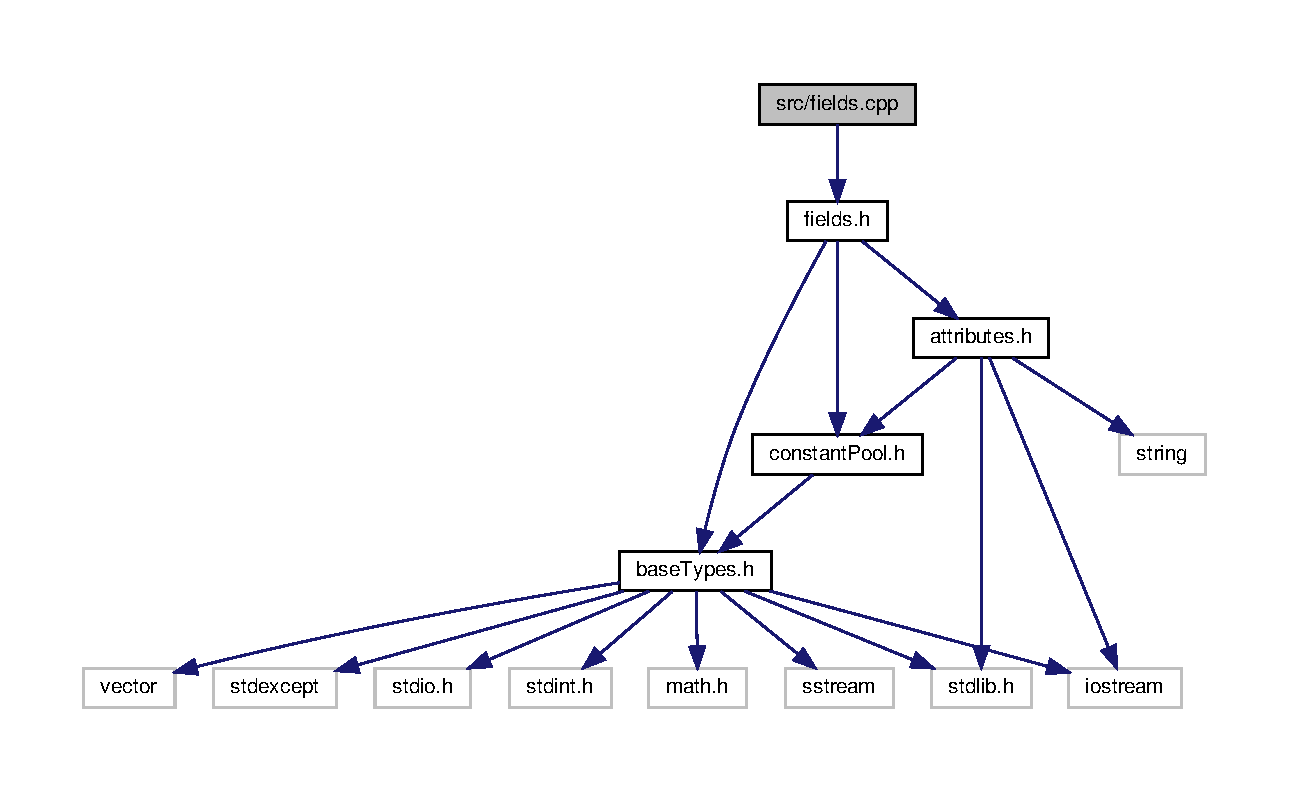
\includegraphics[width=350pt]{fields_8cpp__incl}
\end{center}
\end{figure}
\subsection*{Funções}
\begin{DoxyCompactItemize}
\item 
\mbox{\Hypertarget{fields_8cpp_a3bba8cdcee17336a5484fb8a9d4bcd92}\label{fields_8cpp_a3bba8cdcee17336a5484fb8a9d4bcd92}} 
void {\bfseries print\+Field} (\hyperlink{structfield__info}{field\+\_\+info} f, \hyperlink{structcp__info}{cp\+\_\+info} $\ast$cp, int index)
\item 
void \hyperlink{fields_8cpp_a51b92b23bc1d716b7497c2574577c563}{print\+Fields} (\hyperlink{structfield__info}{field\+\_\+info} $\ast$f, \hyperlink{structcp__info}{cp\+\_\+info} $\ast$cp, int length)
\begin{DoxyCompactList}\small\item\em Fuunção que chama print\+Field o número de vezes determinado por \char`\"{}length\char`\"{}. \end{DoxyCompactList}\item 
\hyperlink{structfield__info}{field\+\_\+info} \hyperlink{fields_8cpp_a95a676570bdecf7ee0595e28472f6b4c}{read\+Field} (F\+I\+LE $\ast$fp, \hyperlink{structcp__info}{cp\+\_\+info} $\ast$cp)
\begin{DoxyCompactList}\small\item\em Função que lê um campo. \end{DoxyCompactList}\item 
\hyperlink{structfield__info}{field\+\_\+info} $\ast$ \hyperlink{fields_8cpp_a0a6c2187c6709928ac89c55afec60703}{read\+Fields} (F\+I\+LE $\ast$fp, int length, \hyperlink{structcp__info}{cp\+\_\+info} $\ast$cp)
\begin{DoxyCompactList}\small\item\em Função que aloca \hyperlink{structfield__info}{field\+\_\+info} espaço e chama read\+Field \char`\"{}lenght\char`\"{} vezes. \end{DoxyCompactList}\item 
string \hyperlink{fields_8cpp_a8b0a792b5f197e376c9f92ec12fda1d8}{get\+Field\+Flags} (unsigned short flags)
\begin{DoxyCompactList}\small\item\em Função para mostrar as flags dos campos. \end{DoxyCompactList}\end{DoxyCompactItemize}


\subsection{Descrição detalhada}
\hyperlink{fields_8cpp}{fields.\+cpp} 

Módulo responsável pela manipulação dos campos existentes no arquivo .class 

\subsection{Documentação das funções}
\mbox{\Hypertarget{fields_8cpp_a8b0a792b5f197e376c9f92ec12fda1d8}\label{fields_8cpp_a8b0a792b5f197e376c9f92ec12fda1d8}} 
\index{fields.\+cpp@{fields.\+cpp}!get\+Field\+Flags@{get\+Field\+Flags}}
\index{get\+Field\+Flags@{get\+Field\+Flags}!fields.\+cpp@{fields.\+cpp}}
\subsubsection{\texorpdfstring{get\+Field\+Flags()}{getFieldFlags()}}
{\footnotesize\ttfamily string get\+Field\+Flags (\begin{DoxyParamCaption}\item[{unsigned short}]{flags }\end{DoxyParamCaption})}



Função para mostrar as flags dos campos. 


\begin{DoxyParams}{Parâmetros}
{\em flags} & Flags em haxadecimal que serão convertidas para string. \\
\hline
\end{DoxyParams}
\mbox{\Hypertarget{fields_8cpp_a51b92b23bc1d716b7497c2574577c563}\label{fields_8cpp_a51b92b23bc1d716b7497c2574577c563}} 
\index{fields.\+cpp@{fields.\+cpp}!print\+Fields@{print\+Fields}}
\index{print\+Fields@{print\+Fields}!fields.\+cpp@{fields.\+cpp}}
\subsubsection{\texorpdfstring{print\+Fields()}{printFields()}}
{\footnotesize\ttfamily void print\+Fields (\begin{DoxyParamCaption}\item[{\hyperlink{structfield__info}{field\+\_\+info} $\ast$}]{f,  }\item[{\hyperlink{structcp__info}{cp\+\_\+info} $\ast$}]{cp,  }\item[{int}]{length }\end{DoxyParamCaption})}



Fuunção que chama print\+Field o número de vezes determinado por \char`\"{}length\char`\"{}. 


\begin{DoxyParams}{Parâmetros}
{\em f} & Struct que contém informação dos campos. \\
\hline
{\em cp} & Ponteiro para pool de constantes. \\
\hline
{\em length} & Define o número de chamadas à print\+Field. \\
\hline
\end{DoxyParams}
\mbox{\Hypertarget{fields_8cpp_a95a676570bdecf7ee0595e28472f6b4c}\label{fields_8cpp_a95a676570bdecf7ee0595e28472f6b4c}} 
\index{fields.\+cpp@{fields.\+cpp}!read\+Field@{read\+Field}}
\index{read\+Field@{read\+Field}!fields.\+cpp@{fields.\+cpp}}
\subsubsection{\texorpdfstring{read\+Field()}{readField()}}
{\footnotesize\ttfamily \hyperlink{structfield__info}{field\+\_\+info} read\+Field (\begin{DoxyParamCaption}\item[{F\+I\+LE $\ast$}]{fp,  }\item[{\hyperlink{structcp__info}{cp\+\_\+info} $\ast$}]{cp }\end{DoxyParamCaption})}



Função que lê um campo. 


\begin{DoxyParams}{Parâmetros}
{\em fp} & Ponteiro para arquivo .class. \\
\hline
{\em cp} & Ponteiro para pool de constantes. \\
\hline
\end{DoxyParams}
\mbox{\Hypertarget{fields_8cpp_a0a6c2187c6709928ac89c55afec60703}\label{fields_8cpp_a0a6c2187c6709928ac89c55afec60703}} 
\index{fields.\+cpp@{fields.\+cpp}!read\+Fields@{read\+Fields}}
\index{read\+Fields@{read\+Fields}!fields.\+cpp@{fields.\+cpp}}
\subsubsection{\texorpdfstring{read\+Fields()}{readFields()}}
{\footnotesize\ttfamily \hyperlink{structfield__info}{field\+\_\+info} $\ast$ read\+Fields (\begin{DoxyParamCaption}\item[{F\+I\+LE $\ast$}]{fp,  }\item[{int}]{length,  }\item[{\hyperlink{structcp__info}{cp\+\_\+info} $\ast$}]{cp }\end{DoxyParamCaption})}



Função que aloca \hyperlink{structfield__info}{field\+\_\+info} espaço e chama read\+Field \char`\"{}lenght\char`\"{} vezes. 


\begin{DoxyParams}{Parâmetros}
{\em fp} & Ponteiro para arquivo .class. \\
\hline
{\em cp} & Ponteiro para pool de constantes. \\
\hline
{\em length} & Define o número de chamadas à read\+Field. \\
\hline
\end{DoxyParams}

\hypertarget{frame_8cpp}{}\section{Referência ao ficheiro src/frame.cpp}
\label{frame_8cpp}\index{src/frame.\+cpp@{src/frame.\+cpp}}
{\ttfamily \#include \char`\"{}frame.\+h\char`\"{}}\newline
Diagrama de dependências de inclusão para frame.\+cpp\+:
\nopagebreak
\begin{figure}[H]
\begin{center}
\leavevmode
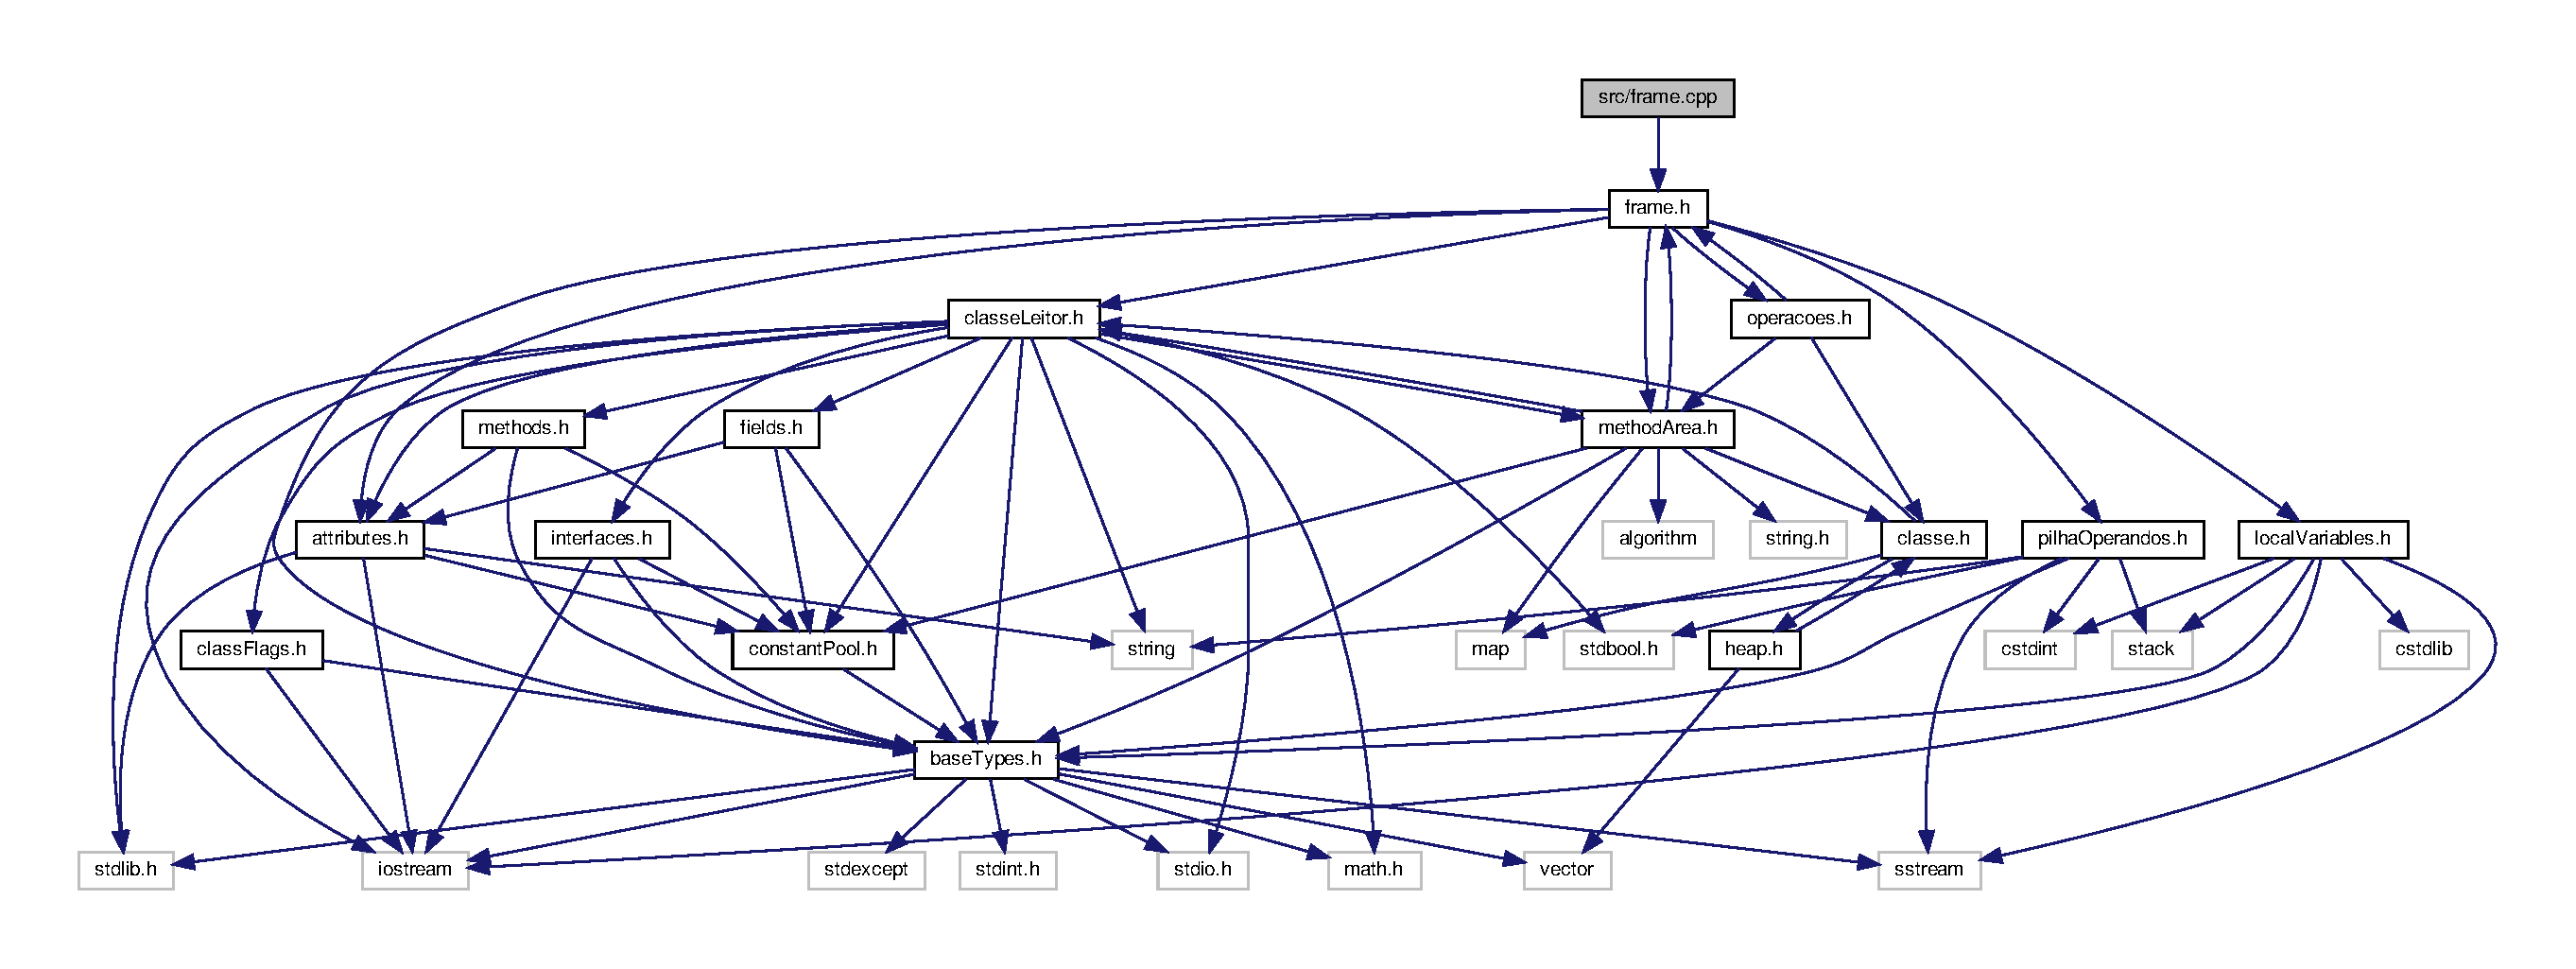
\includegraphics[width=350pt]{frame_8cpp__incl}
\end{center}
\end{figure}

\hypertarget{heap_8cpp}{}\section{Referência ao ficheiro src/heap.cpp}
\label{heap_8cpp}\index{src/heap.\+cpp@{src/heap.\+cpp}}
{\ttfamily \#include \char`\"{}heap.\+h\char`\"{}}\newline
Diagrama de dependências de inclusão para heap.\+cpp\+:\nopagebreak
\begin{figure}[H]
\begin{center}
\leavevmode
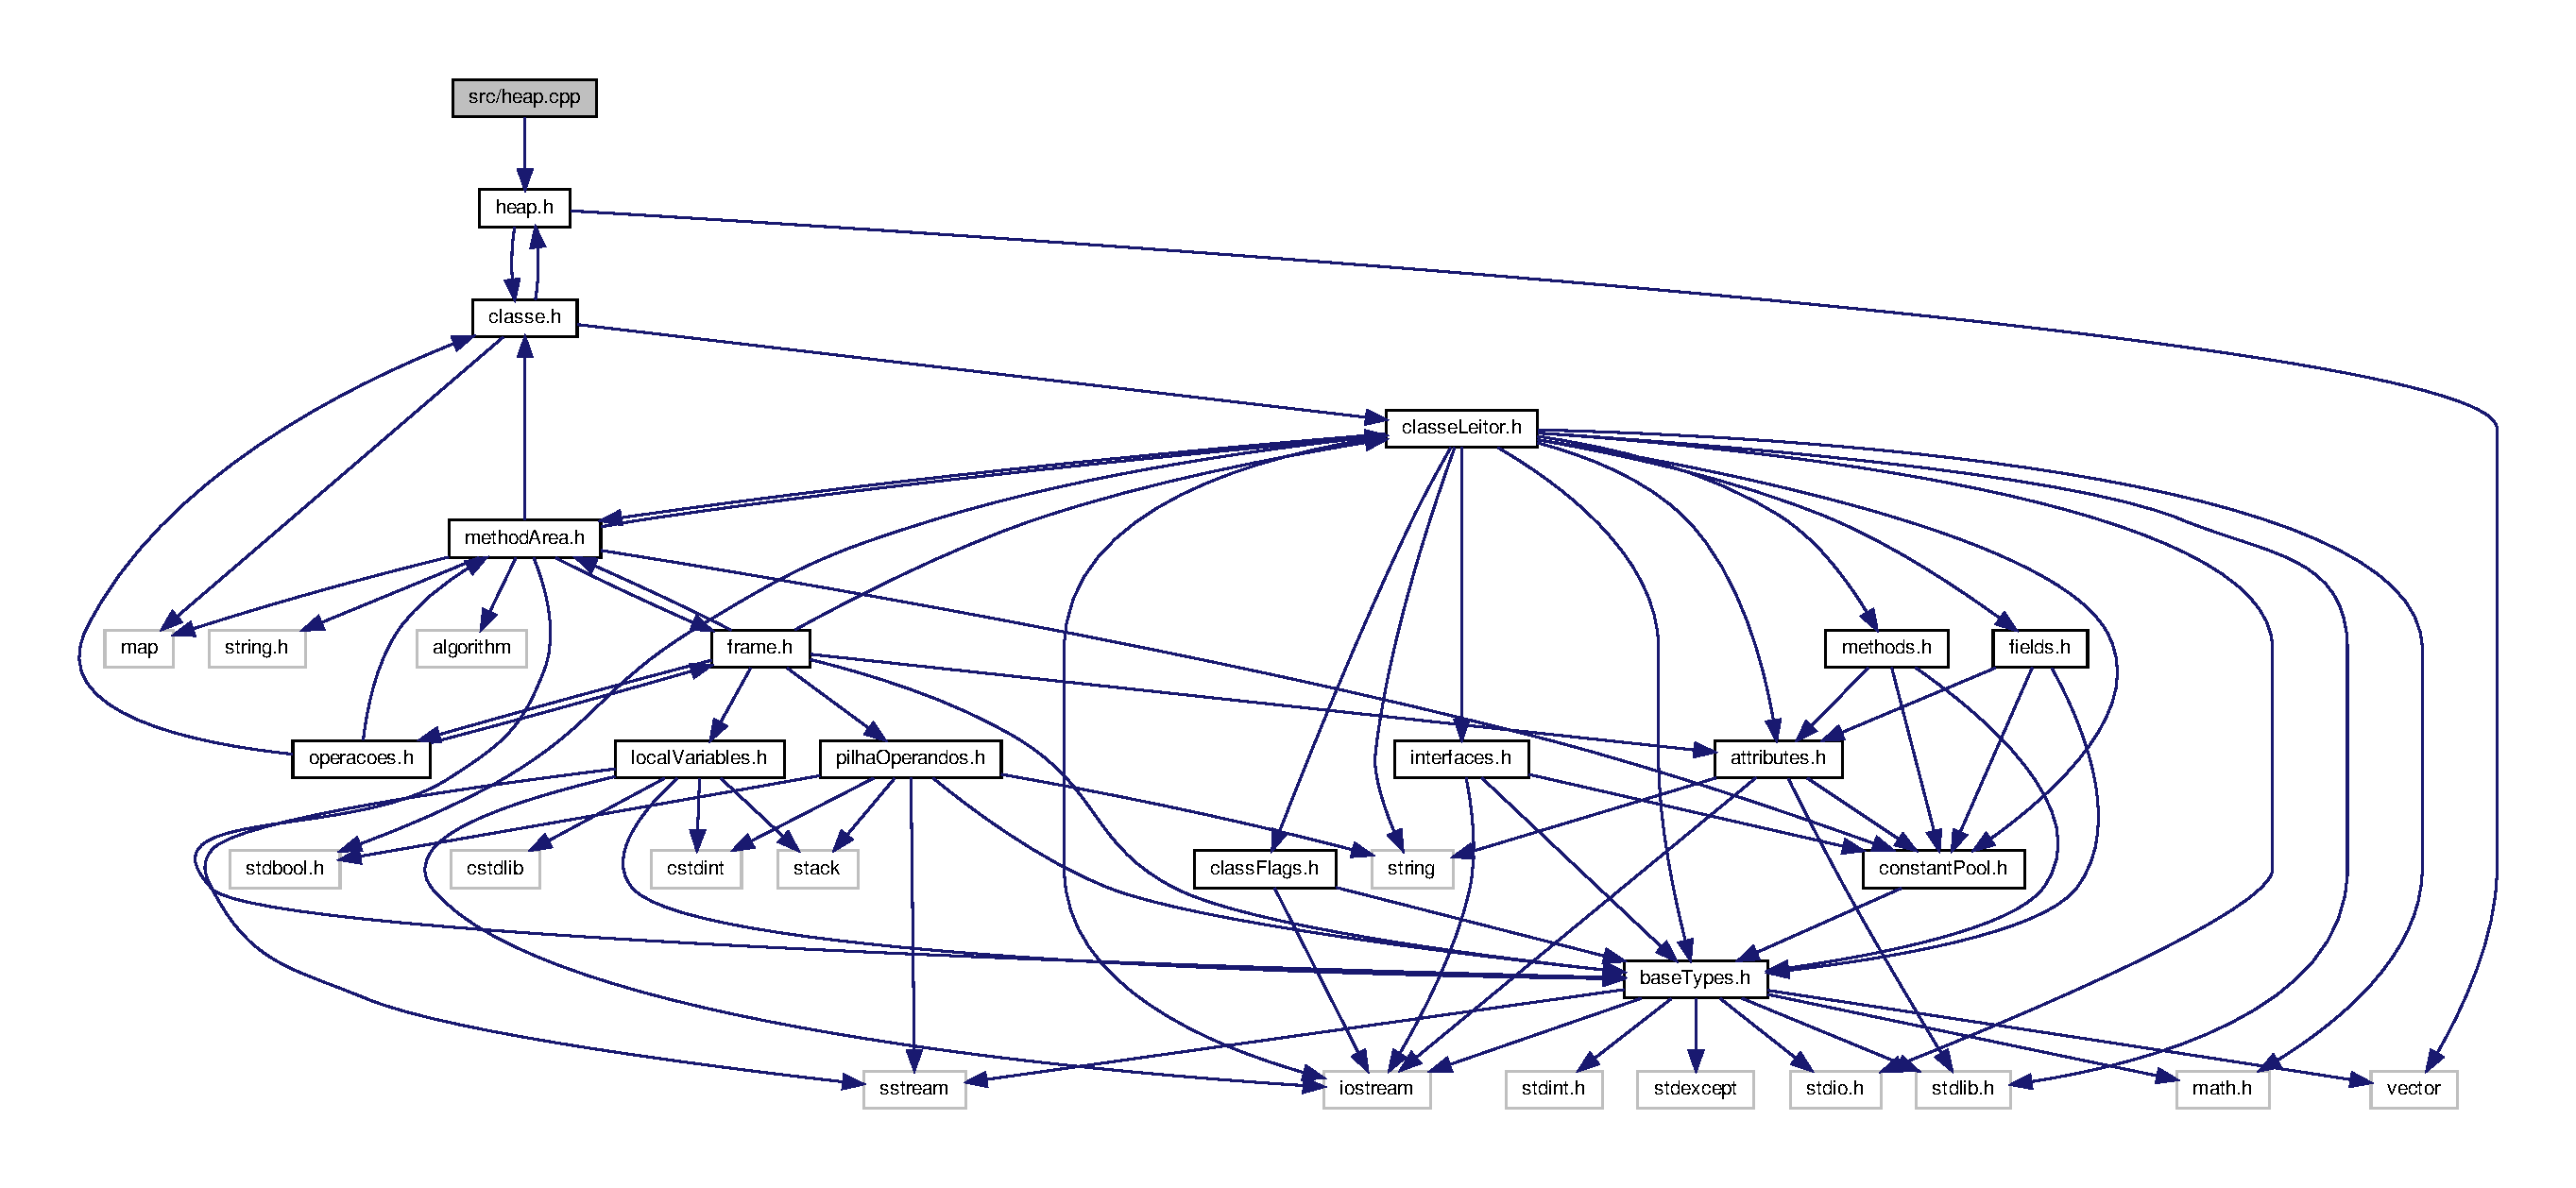
\includegraphics[width=350pt]{heap_8cpp__incl}
\end{center}
\end{figure}

\hypertarget{localVariables_8cpp}{}\section{Referência ao ficheiro src/local\+Variables.cpp}
\label{localVariables_8cpp}\index{src/local\+Variables.\+cpp@{src/local\+Variables.\+cpp}}


Local\+Variables.\+cpp.  


{\ttfamily \#include \char`\"{}local\+Variables.\+h\char`\"{}}\newline
Diagrama de dependências de inclusão para local\+Variables.\+cpp\+:
\nopagebreak
\begin{figure}[H]
\begin{center}
\leavevmode
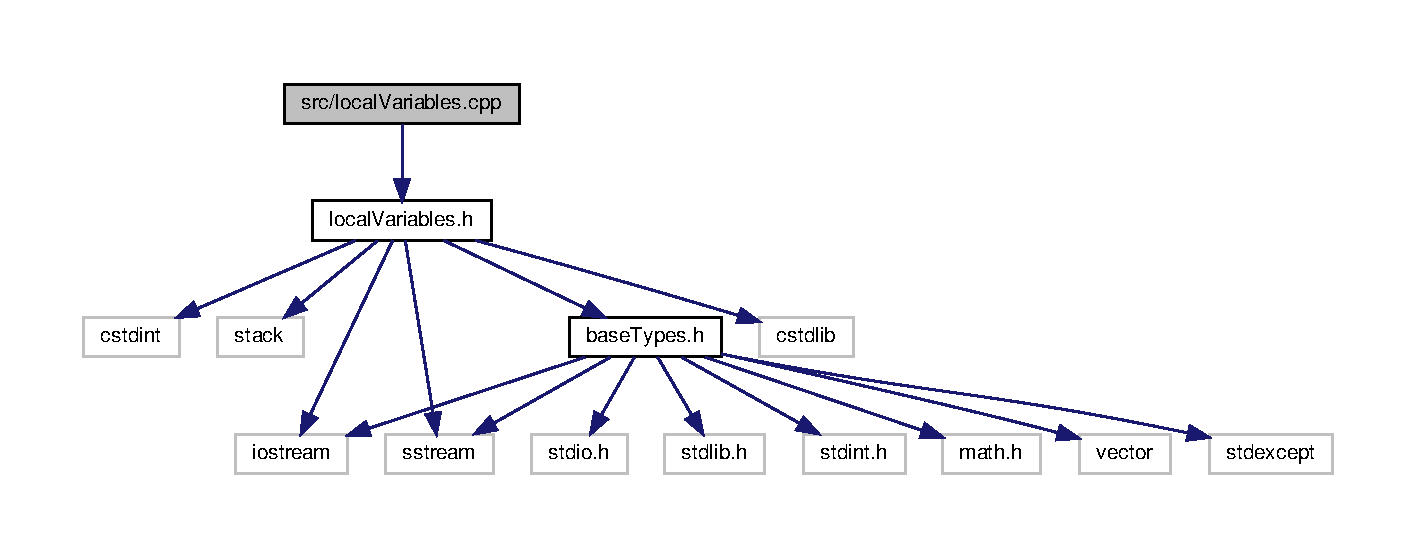
\includegraphics[width=350pt]{localVariables_8cpp__incl}
\end{center}
\end{figure}


\subsection{Descrição detalhada}
Local\+Variables.\+cpp. 


%--- End generated contents ---

% Index
\backmatter
\newpage
\phantomsection
\clearemptydoublepage
\addcontentsline{toc}{chapter}{Índice}
\printindex

\end{document}
